\chapter{Cross-Section Extraction}
\label{ch:extraction}



This chapter describes the full procedure used to calculate the total $\nu_\mu$ \acrshort{cc} inclusive cross section on argon, as well as the single- and double-differential cross sections in muon momentum and angle. Only statistical uncertainties will be taken into account in this chapter. Systematic uncertainties will be discussed in Chapter~\ref{ch:systematics}, and the final results are shown in Chapter~\ref{ch:cross_section_results}. 

The MicroBooNE baseline simulation uses the ``\tuneone'' configuration, and the cross section will be extracted using the efficiency and the backgrounds estimated according to this simulation. The data extracted cross section will be denoted as $\sigma$ in the following. Equivalently the cross section from simulation will be denoted as $\sigma_\text{MC}$. 

Section~\ref{sec:xsec_calculation} shows an overview on the cross section calculation, while Section~\ref{sec:total_xsec} describes the extraction of the total cross section. Similarly, Sections~\ref{sec:mumom_xsec},~\ref{sec:muangle_xsec} and~\ref{sec:mumom_muangle_xsec} describe the extraction of the two single-differential cross sections and the double-differential cross section in $p_\mu$ and $\cos\theta_\mu$ respectively.

%**********************************************************
\section{Cross-Section Calculation}
\label{sec:xsec_calculation}

The total flux-integrated cross section is calculated using the following equation:

\begin{equation}
\label{eq:xsec_total}
\sigma = \frac{N - B}{\epsilon \cdot T \cdot \Phi_{\nu_\mu}},
\end{equation}
where $N$ is the total number of selected data events, $B$ is the number of selected background events (from simulation and beam-off data), $\epsilon$ is the efficiency of the event selection (overall, including acceptance), $T$ is the number of target nucleons and $\Phi_{\nu_\mu}$ is the \acrshort{bnb} muon neutrino flux integrated over energy and scaled to the corresponding \acrshort{pot} received for the analysis.

In addition to a total cross section, the result is also reported in terms of a differential cross section as a function of muon kinematics, such as the muon momentum $p_\mu$ and the cosine of the muon angle $\theta_\mu$ with respect to the beam direction. In this case, the signal and background event rates, as well as the efficiencies, are binned as a function of muon momentum or angle and the single-differential cross sections in bin $i$ are calculated as

\begin{equation}
\label{eq:xsec_differential}
\begin{split}
\left ( \frac{d\sigma}{dp_\mu} \right )_i &= \frac{N_i - B_i}{\tilde{\epsilon}_i \cdot T \cdot \Phi_{\nu_\mu} \cdot (\Delta p_\mu)_i}, \\
\left ( \frac{d\sigma}{d\cos\theta_\mu} \right )_i &= \frac{N_i - B_i}{\tilde{\epsilon}_i \cdot T \cdot \Phi_{\nu_\mu} \cdot (\Delta \cos\theta_\mu)_i},
\end{split}
\end{equation}

where $N_i$, $B_i$ and $\tilde{\epsilon}_i$ are the number of candidate events, the number of background events and the efficiency in bin $i$, respectively. $(\Delta p_\mu)_i$ and $(\Delta \cos\theta_\mu)_i$ are the bin widths for bin $i$ in the $p_\mu$ and $\cos\theta_\mu$ distributions, respectively. 

Similarly, the double-differential cross section is extracted according to
\begin{equation}
\label{eq:xsec_double_differential}
\left ( \frac{d^2\sigma}{dp_\mu d\cos\theta_\mu} \right )_{i} = \frac{N_{i} - B_{i}}{\tilde{\epsilon}_{i} \cdot T \cdot \Phi_{\nu_\mu} \cdot (\Delta p_\mu\cdot \Delta \cos\theta_\mu)_i},
\end{equation}
where $(\Delta p_\mu\cdot \Delta \cos\theta_\mu)_i$ is the $i^\text{th}$ bin area.

All these cross sections are called ``flux integrated'' as they include neutrinos with different energies (distributed according to the neutrino spectrum at the detector location). In neutrino interaction differential cross-section measurements, no attempt is usually made to correct for the incoming neutrino flux in each bin of the measurement. Instead, each bin is normalised by the total integrated flux. Because $\Phi_{\nu_\mu}$ is the integrated neutrino flux at the detector location, the result is experiment dependent. Indeed, the shape of the incoming neutrino flux must be made available with the measurement, such that a model can be convoluted with the flux to be comparable to the result.

A specific problem arises in the measurement of a differential cross section that is related to the resolution on $p_\mu$ and $\cos\theta_\mu$. If the resolution on these quantities is larger or of the same order than the bin dimension, migration of events between neighbouring bins is expected, affecting the shape of the differential cross section for the reconstructed events. The binning used in this analysis, described below, is made in order to guarantee small bin-to-bin migrations by choosing bin width larger than the resolution. In order to understand the bin-to-bin migrations a smearing matrix $S$ is constructed, allowing to convert the number of true events in a true bin $j$, to the number of observed events in a reconstructed bin $i$ such that:
\begin{equation}
\label{eq:smearing_matrix_2d}
\nu_i = \sum_{j=1}^{M} S_{ij} \mu_j,
\end{equation}
where $S$ is given by:
\begin{equation}
S_{ij} = P(\text{observed in bin}\, i \,|\, \text{true value in bin}\, j),
\end{equation}
and $\nu_i$ and $\mu_j$ are the number of events in the reconstructed bin $i$ and true bin $j$, respectively, and $M$ is the total number of bins.
Smeared data can be analysed in two ways: 
\begin{description}
\item[Forward Folding] With this approach, the data distribution is presented in reconstructed observables. A theoretical spectrum can be smeared from truth quantities to reconstructed observables, and then be compared directly to the data. The migration matrix, needed to smear the theoretical spectrum, has to be provided alongside the cross-section distributions, in order for people outside the experiment to be able to make model comparisons. This approach does not allow a direct comparison to other experiments, which may provide  forward-folded distributions with different smearing matrices, or forward-folded ones.
\item[Unfolding] This approach corrects for smearing and other detector effects by trying to deconvolve those effects in order to get to the true underlying distribution. This method allows a direct comparison to unfolded measurements from other experiments. 
\end{description}
Although the majority of experiments use the unfolding approach, the cross section presented in this thesis is extracted using the forward-folding method. The unfolding procedure can introduce biases in the cross-section extraction, can add correlations between the data points and presents failures when testing the goodness of a fit to a certain model, as shown in~\cite{forward_folding}.
In this work, a comparison between a predicted theory and the observed data is performed at the level of the smeared theory with the actual data, rather than between the pure true and the unfolded data. This comparison between theoretical models and data is possible if the smearing matrix is published with the data, as it will be done with this analysis.
While the efficiency $\epsilon_j$ in true bin $j$ is given by the ratio of the number of selected signal  events $N^\text{sel}_j$ and the number of generated signal events $N^\text{gen}_j$ in true bin $j$:
\begin{equation}
\label{eq:eff_true}
{\epsilon}_j = \frac{ N^\text{sel}_j}{ N^\text{gen}_j},
\end{equation}
for this analysis the true distributions have to be smeared in order to evaluate the efficiency in reconstructed bin $i$:
\begin{equation}
\label{eq:eff_smear}
\tilde{\epsilon}_i = \frac{ \sum_{j=1}^{M} S_{ij}N^\text{sel}_j}{ \sum_{j=1}^{M} S_{ij}N^\text{gen}_j}.
\end{equation}
This efficiency is used to extract the cross section using formulas~\eqref{eq:xsec_differential} and~\eqref{eq:xsec_double_differential}.
where $N^\text{sel}_j$ is the number of signal selected events in true bin $j$, and $N^\text{gen}_j$ is the number of generated signal events in true bin $j$. 






\subsection{\acrshort{bnb} Neutrino Integrated Flux}
\label{sec:flux}

The \acrshort{bnb} $\nu_\mu$ flux in neutrino mode running is shown in Figure \ref{fig:flux_energy_range}. The flux is simulated using the MiniBooNE framework as described in~\cite{miniboone_flux}. The total integrated flux scaled to $1.592 \times 10^{20}$ \acrshort{pot} is
\begin{equation}
\Phi_{\nu_\mu} = 1.16859 \times 10^{11} \, \text{cm}^{-2}.
\end{equation}
The mean neutrino energy for the \acrshort{bnb} flux is 
\begin{equation}
\label{eq:nu_energy_range}
\left < E_{\nu_{\mu}} \right > = 823 \, \text{MeV},
\end{equation}
with 68\% of the values falling into the energy range of $823 - 498 = 325$ MeV and $823 + 502 = 1325$ MeV.
This energy range is not used for the analysis but is used for comparison to other measurements. Tabulated values of the \acrshort{bnb} $\nu_\mu$ flux as a function of neutrino energy are available in~\cite{flux_note}.

\begin{figure}[]
\centering
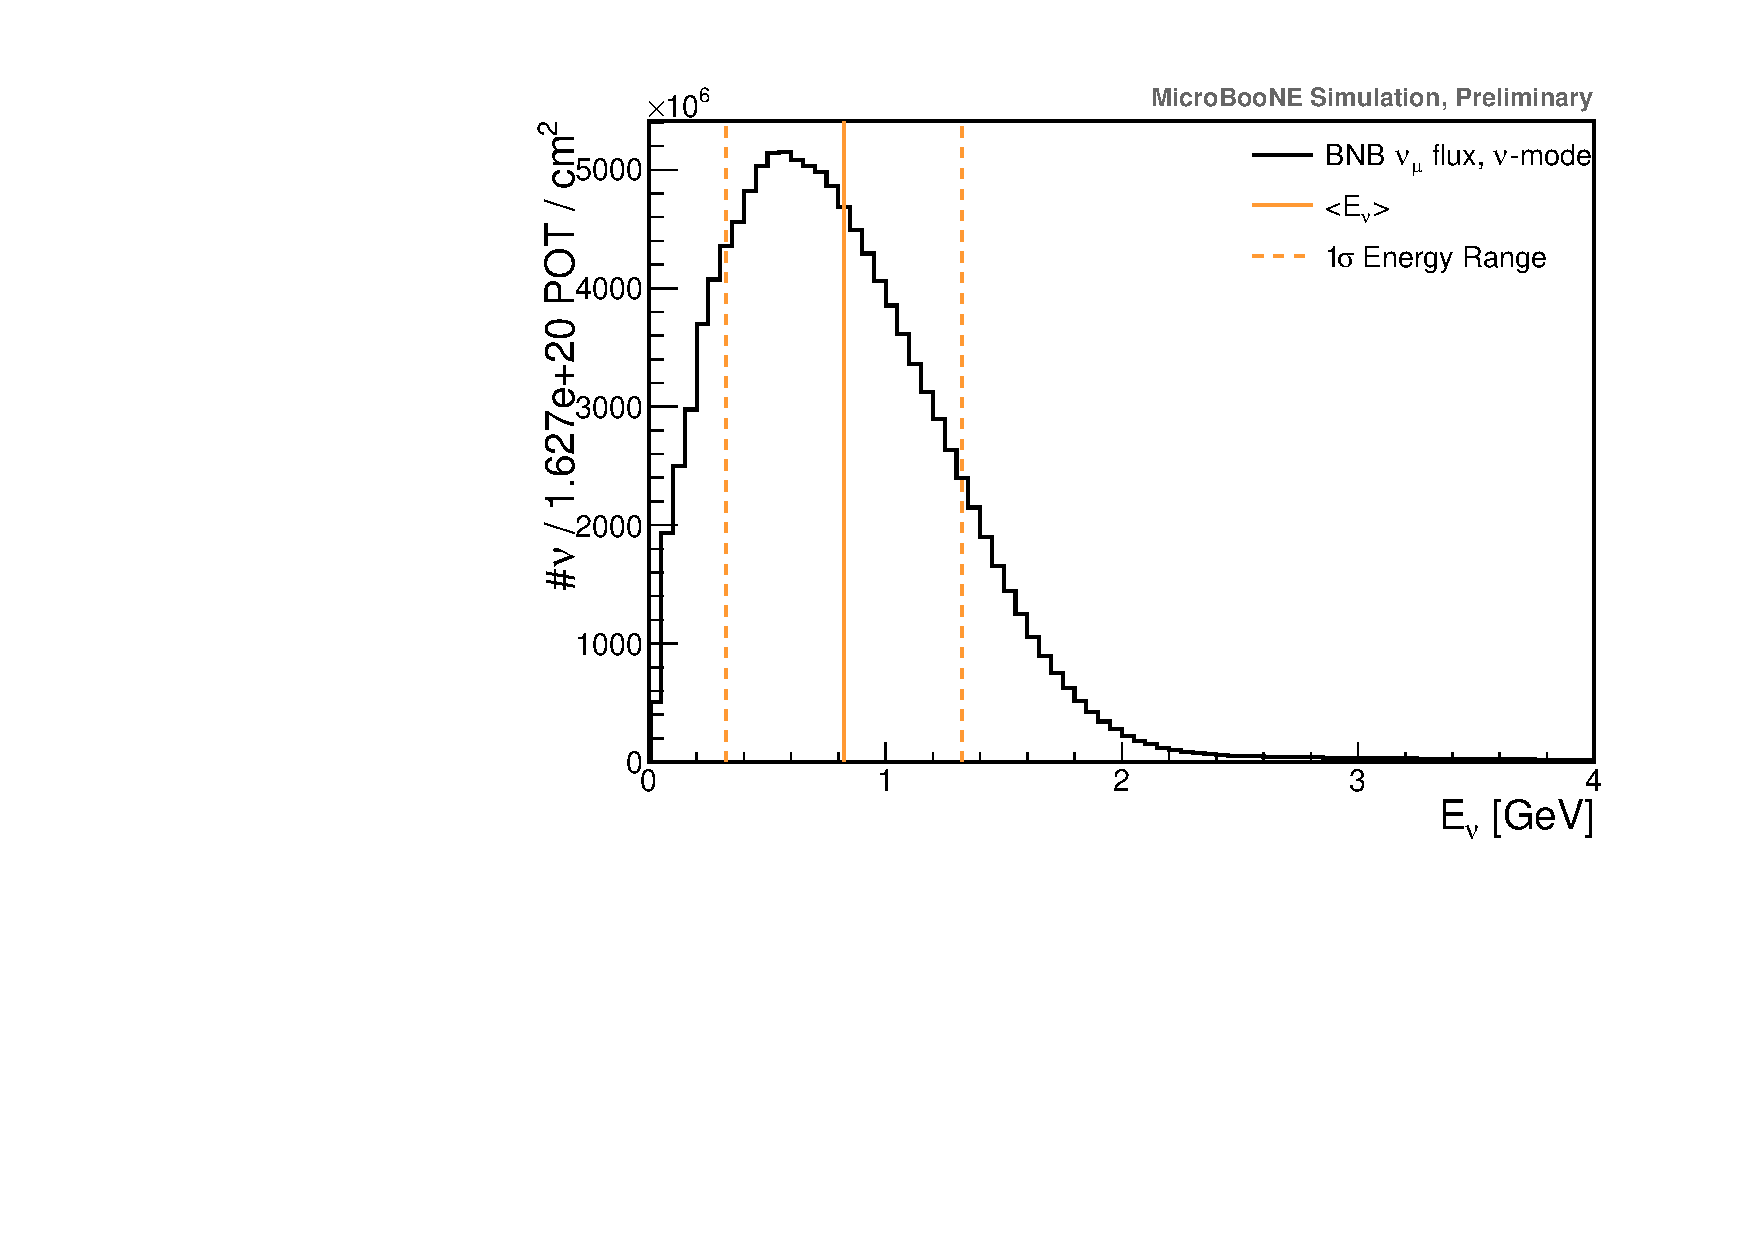
\includegraphics[width=.70\textwidth]{images/flux_energy_range}
\caption[\acrshort{bnb} $\nu_\mu$ Flux at MicroBooNE]{\acrshort{bnb} $\nu_\mu$ flux in neutrino mode at the MicroBooNE detector center, scaled to $1.592 \times 10^{20}$ \acrshort{pot}. The lines mark the mean neutrino energy and the 1$\sigma$ range.}
\label{fig:flux_energy_range}
\end{figure} 



\subsection{Number of Target Nucleons}

The number of target nucleons $T$ in the \acrshort{fv} is calculated as

\begin{equation}
\label{eq:ntarget}
T = \frac{\rho_\text{Ar} \cdot V \cdot N_A \cdot N_\text{nucleons}}{m_\text{mol}},
\end{equation}
where $\rho_\text{Ar}$ is the liquid argon density, $V$ is the \acrshort{fv}, $N_A$ is the Avogadro number, $N_\text{nucleons}$ is the number of nucleons per argon nucleus, and $m_\text{mol}$ is the number of grams per mole of argon. The \acrshort{fv} is split in two sub-volumes, $V_1$ and $V_2$, as previously shown in Figure \ref{fig:fiducial_volume}. The volume is treated as pure argon as the number of contaminants have been measured to be less than one particle per million~\cite{purity_note}. The NIST database at the MicroBooNE measured temperature and pressure was used to calculate the density of liquid argon. The calculated liquid argon density was found to be slightly different ($<1\%$ difference) with respect to the simulated one, as simulation uses the design temperature and pressure, and not the measured ones. This leads to two values for the number of targets, one for the data, and one for the simulation. Using
\begin{equation}
\begin{split}
V_1 &= 2.46175 \times 10^7 \, \text{cm}^3, \\
V_2 &= 6.69596 \times 10^6 \, \text{cm}^3, \\
\rho_\text{Ar}^\text{data} &= 1.3836^{+0.0019}_{-0.0002} \, \text{g}/\text{cm}^3, \\
\rho_\text{Ar}^\text{\acrshort{mc}} &= 1.3954 \, \text{g}/\text{cm}^3, \\
m_\text{mol} &= 39.95 \, \text{g}/\text{mol}, \\
N_A &= 6.022140857(74) \times 10^{23} \, \text{molec}/\text{mol}, \\
N_\text{nucleons} &= 40, \\
\end{split}
\end{equation}
the following values for the number of targets are obtained:
\begin{equation}
\begin{split}
T^\text{data} &= 2.6124^{+0.0036}_{-0.0003} \times 10^{31}, \\
T^\text{\acrshort{mc}} &= 2.6347 \times 10^{31}.
\end{split}
\end{equation}
$T^\text{data}$ will be used to extract the data cross section, while $T^\text{\acrshort{mc}}$ will be used for the \acrshort{mc} predicted cross section. The uncertainties on the number of targets will be discussed in Section~\ref{sec:error_targets}.





\subsection{Analysis Binning}
\label{sec:binning}

The binning for the $p_\mu$ distribution must be determined before moving to the cross-section extraction.
The main strategy used to find the binning is to ensure that the majority of the true values that correspond to the reconstructed values in one bin, fall in the same reconstructed bin. This is done in order to mitigate bin-to-bin migrations. 
Moreover, the binning is chosen such that: there are a similar number of events in each reconstructed bin; the statistical uncertainty is comparable in every bin; the change in the expected cross section within a bin is small; the efficiency stays almost flat inside one bin; the efficiency, averaged over one bin, is not less than 30\%, to avoid having bins with very small efficiency.
The only exceptions are the bins in the backward region of the $\cos\theta_\mu$ distribution ($\cos\theta_\mu < 0$). This region was simply split in two bins, $\cos\theta_\mu \in [-1, -0.5)$ and $\cos\theta_\mu \in [-0.5, 0)$, given the low data statistic in this region.  
The final bin choice for $p_\mu$ is:
\begin{equation}
p_\mu \, \text{bins}: [0.00, 0.18, 0.30, 0.45, 0.77, 1.28, 2.50],
\end{equation}
while for $\cos\theta_\mu$ is:
\begin{equation}
\cos\theta_\mu \, \text{bins}: [-1.00, -0.50, 0.00, 0.27, 0.45, 0.62, 0.76, 0.86, 0.94, 1.00].
\end{equation}
Figures~\ref{fig:true_reco_mumom} and~\ref{fig:true_reco_muangle} show the comparison of simulated and reconstructed variables with a fine binning.
Figures~\ref{fig:true_reco_mumom_rightbin} and~\ref{fig:true_reco_muangle_rightbin} show the same distributions with the final binning, as defined above.

\begin{figure}[]
\centering
\subfloat[][]
   {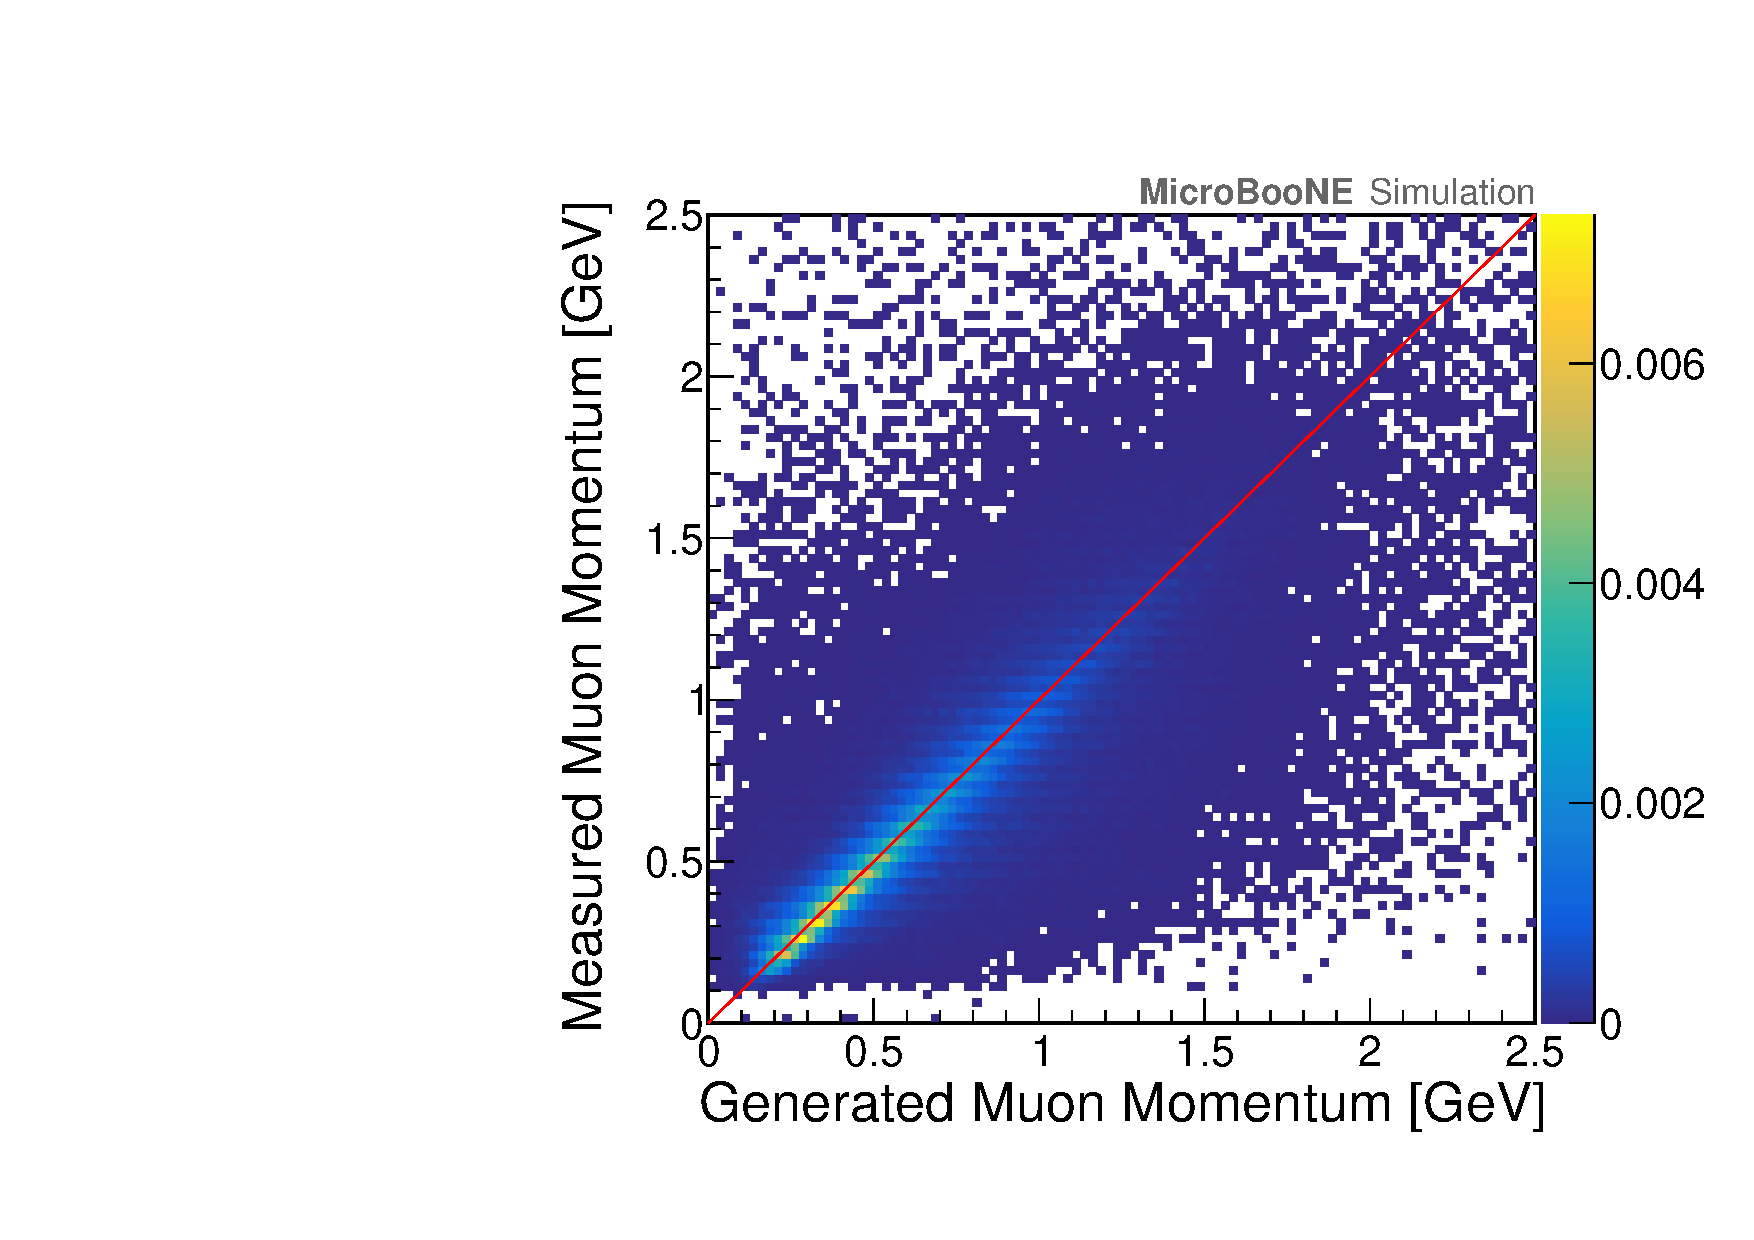
\includegraphics[width=.5\textwidth]{images/BinningPmu/true_reco_mumom}
   \label{fig:true_reco_mumom}}
\subfloat[][]
   {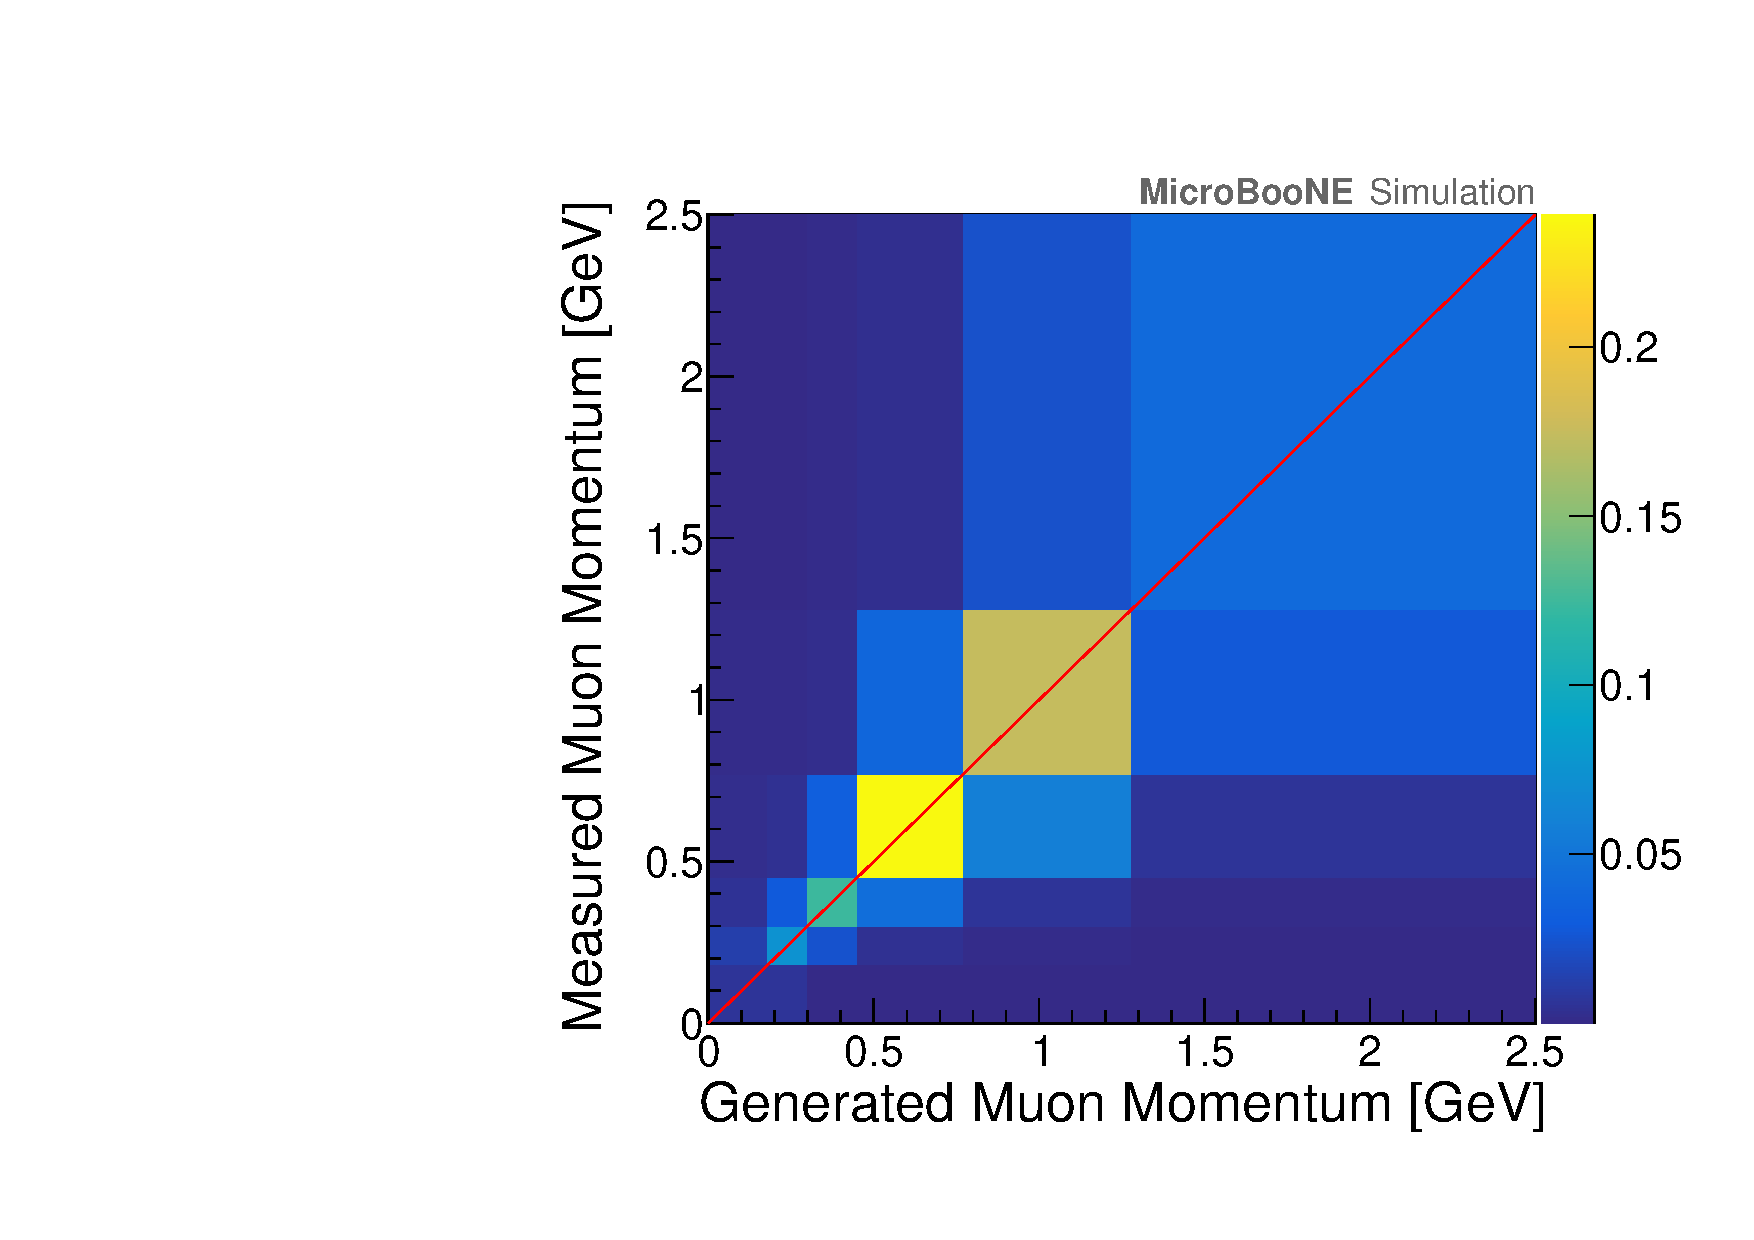
\includegraphics[width=.5\textwidth]{images/BinningPmu/true_reco_mumom_rightbin}
   \label{fig:true_reco_mumom_rightbin}} \\
 \subfloat[][]
   {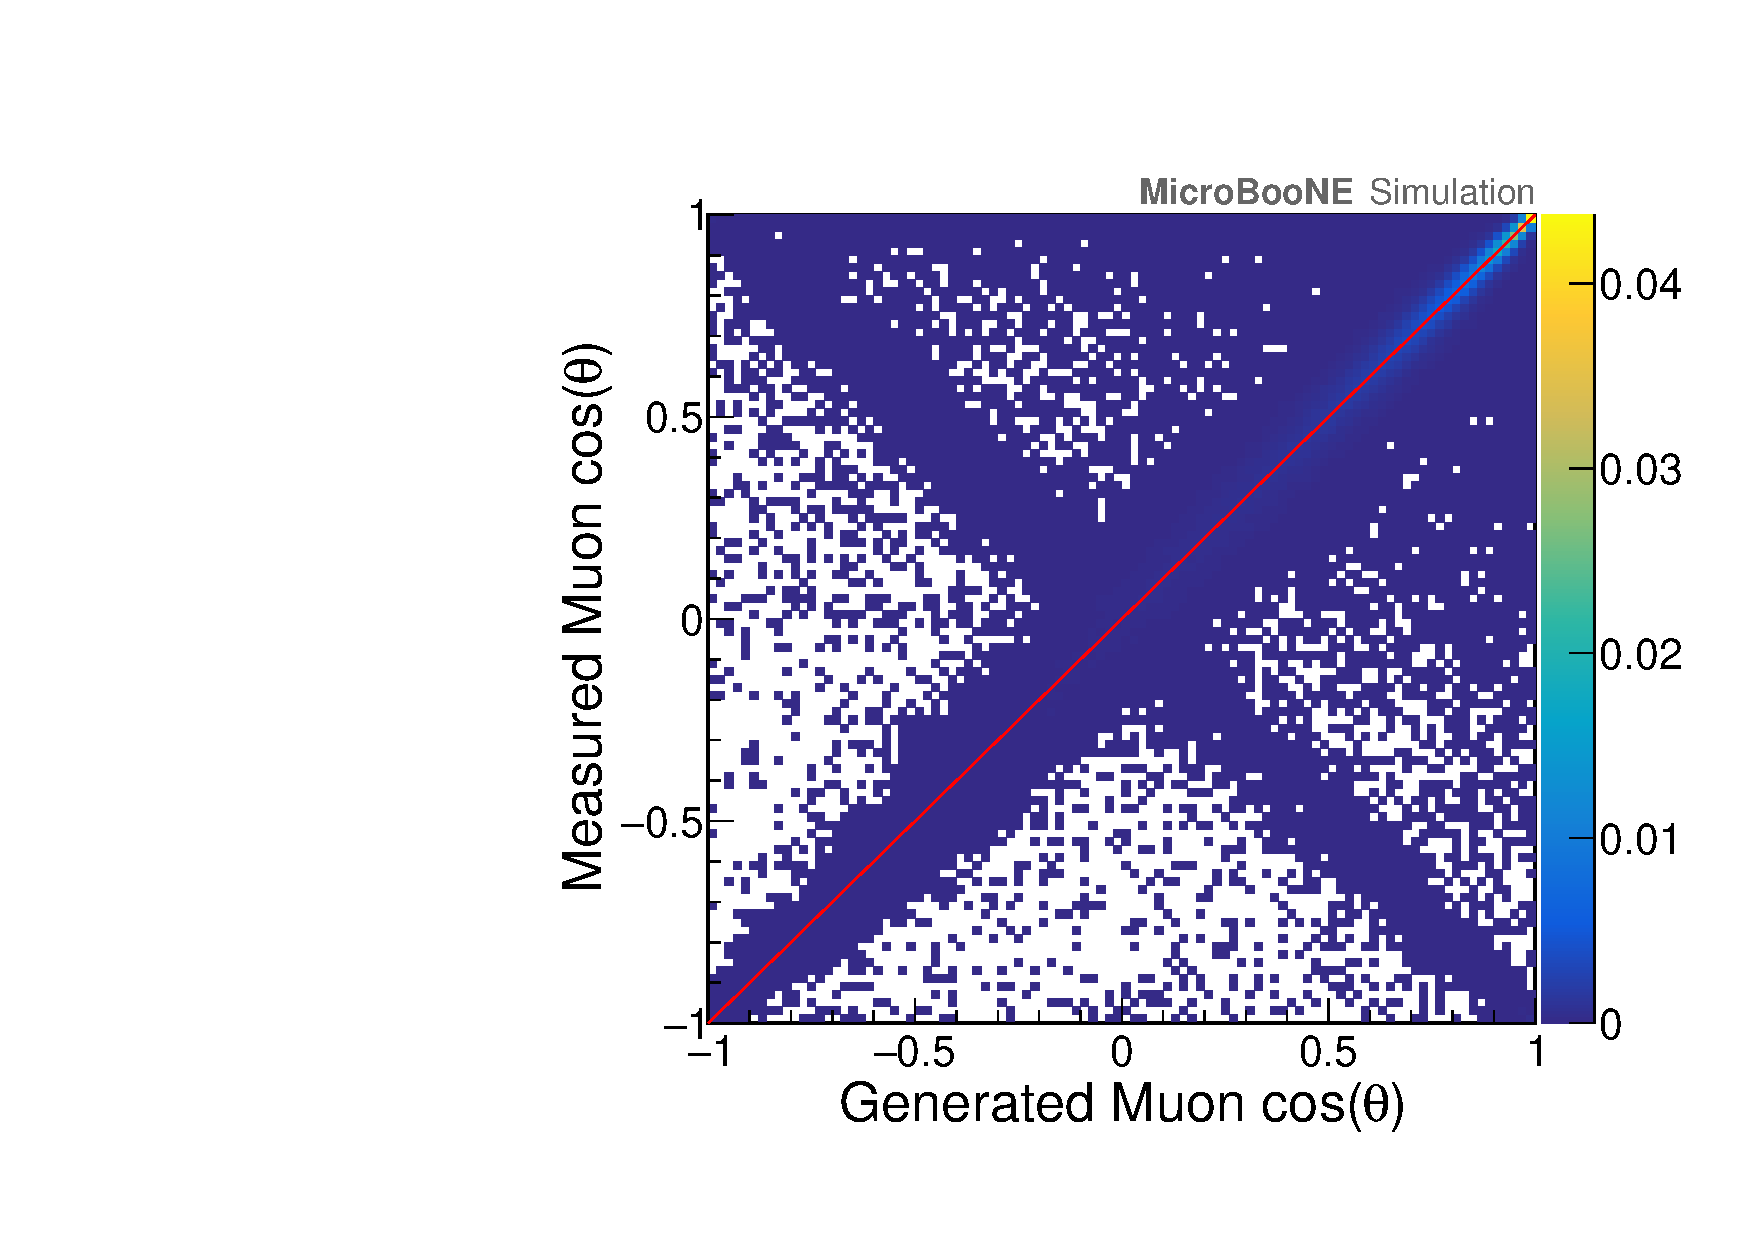
\includegraphics[width=.5\textwidth]{images/BinningCosThetaMu/true_reco_muangle}
   \label{fig:true_reco_muangle}}
\subfloat[][]
   {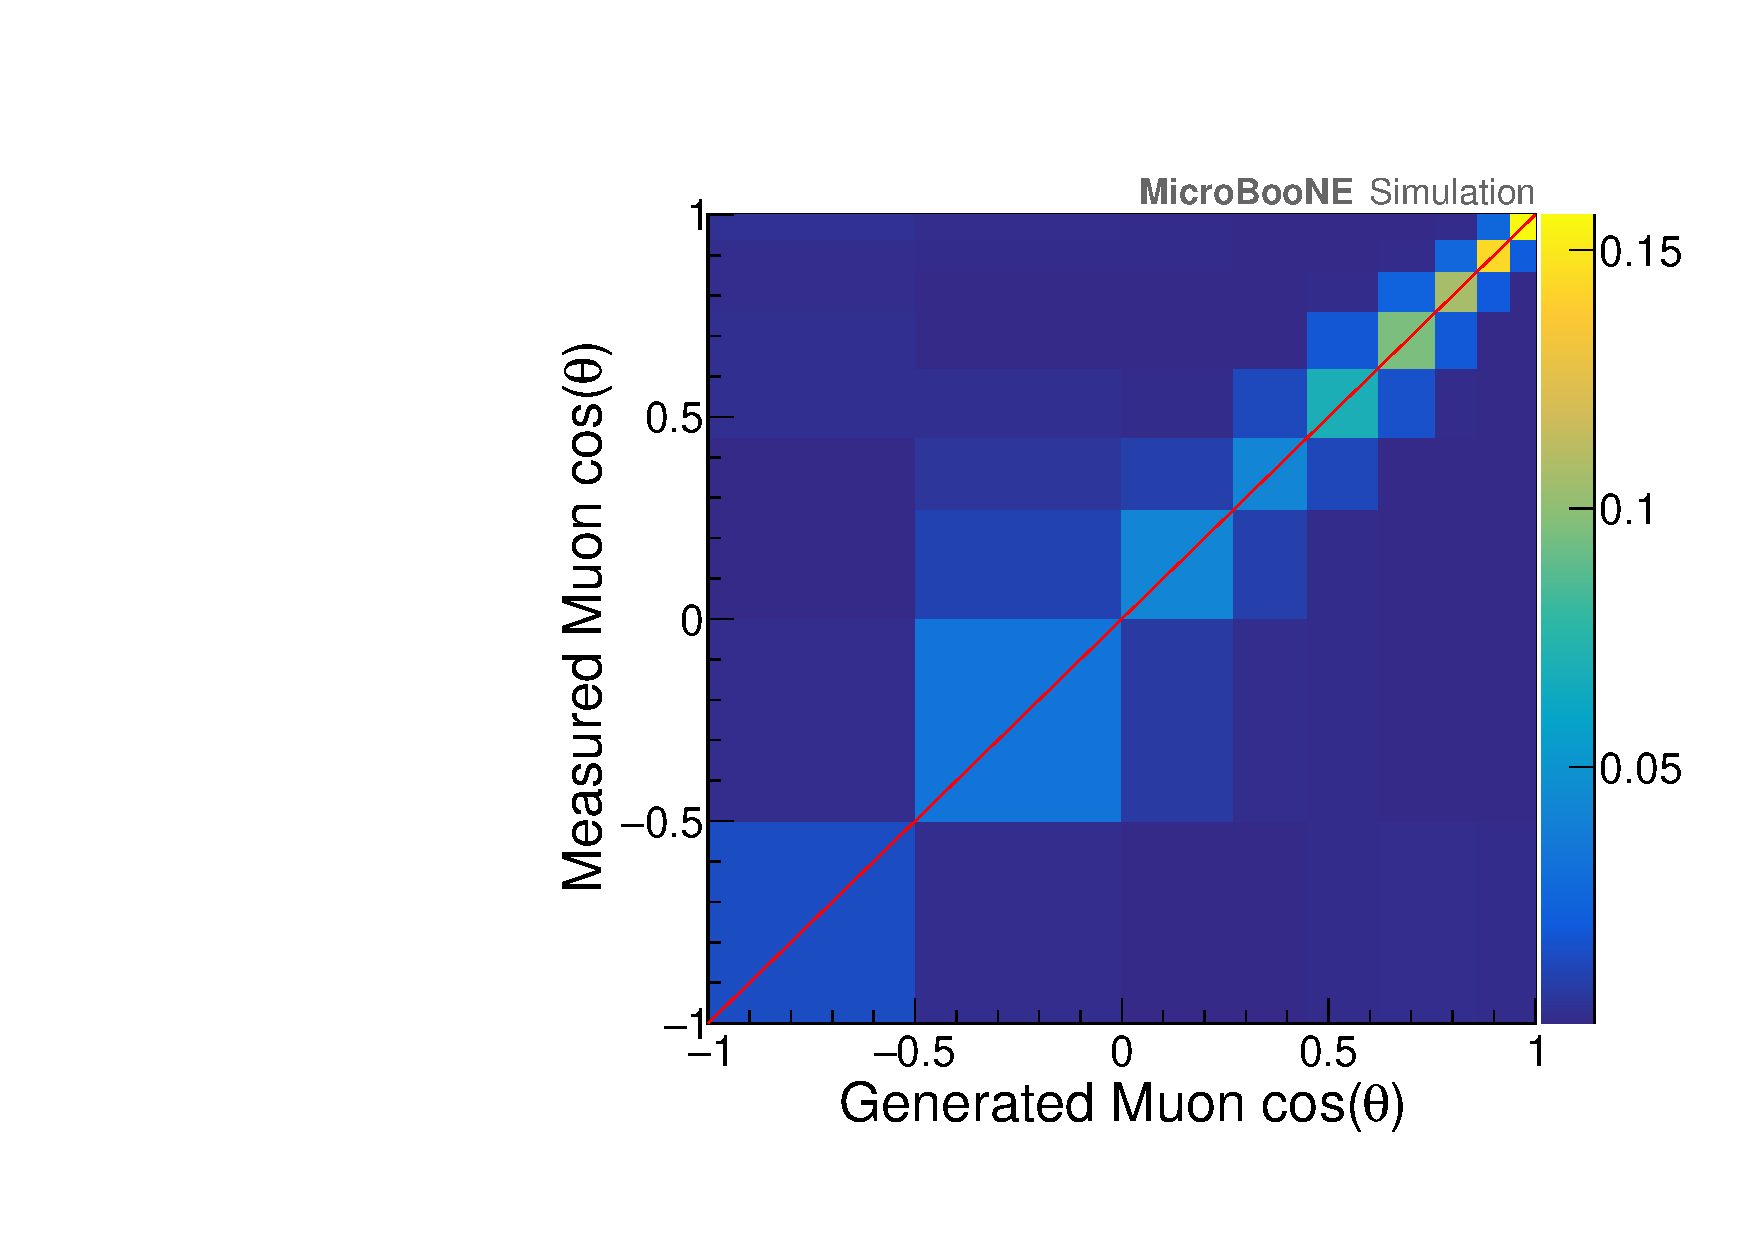
\includegraphics[width=.5\textwidth]{images/BinningCosThetaMu/true_reco_muangle_rightbin}
   \label{fig:true_reco_muangle_rightbin}} \\
\caption[Generated v.s.~Measured Muon Momentum and Angle]{Distribution of the measured v.s.~generated muon momentum and cosine of the muon angle in~\protect\subref{fig:true_reco_mumom} and~\protect\subref{fig:true_reco_muangle}, respectively. The right plots~\protect\subref{fig:true_reco_mumom_rightbin} and~\protect\subref{fig:true_reco_muangle_rightbin} are the same as the left ones but using the new binning defined for the cross section extraction.}
\label{fig:binning}
\end{figure}


For the double differential cross section, a very similar binning for $p_\mu$ and $\cos\theta_\mu$ is used, with some modifications. The same bin boundaries are used, but some of the $p_\mu$ bins are merged, especially in the backward region, to ensure enough statistics in each bin. The binning choice is shown in Figure~\ref{fig:polybins}. The number in each bin represents the bin unique identifier (bin ID). The bin ID will be used for the construction of the smearing matrices and all the covariance matrices. The reader should refer to Figure~\ref{fig:polybins} to understand the bins in all the following matrices.

%\begin{SCfigure}[]
%\centering
%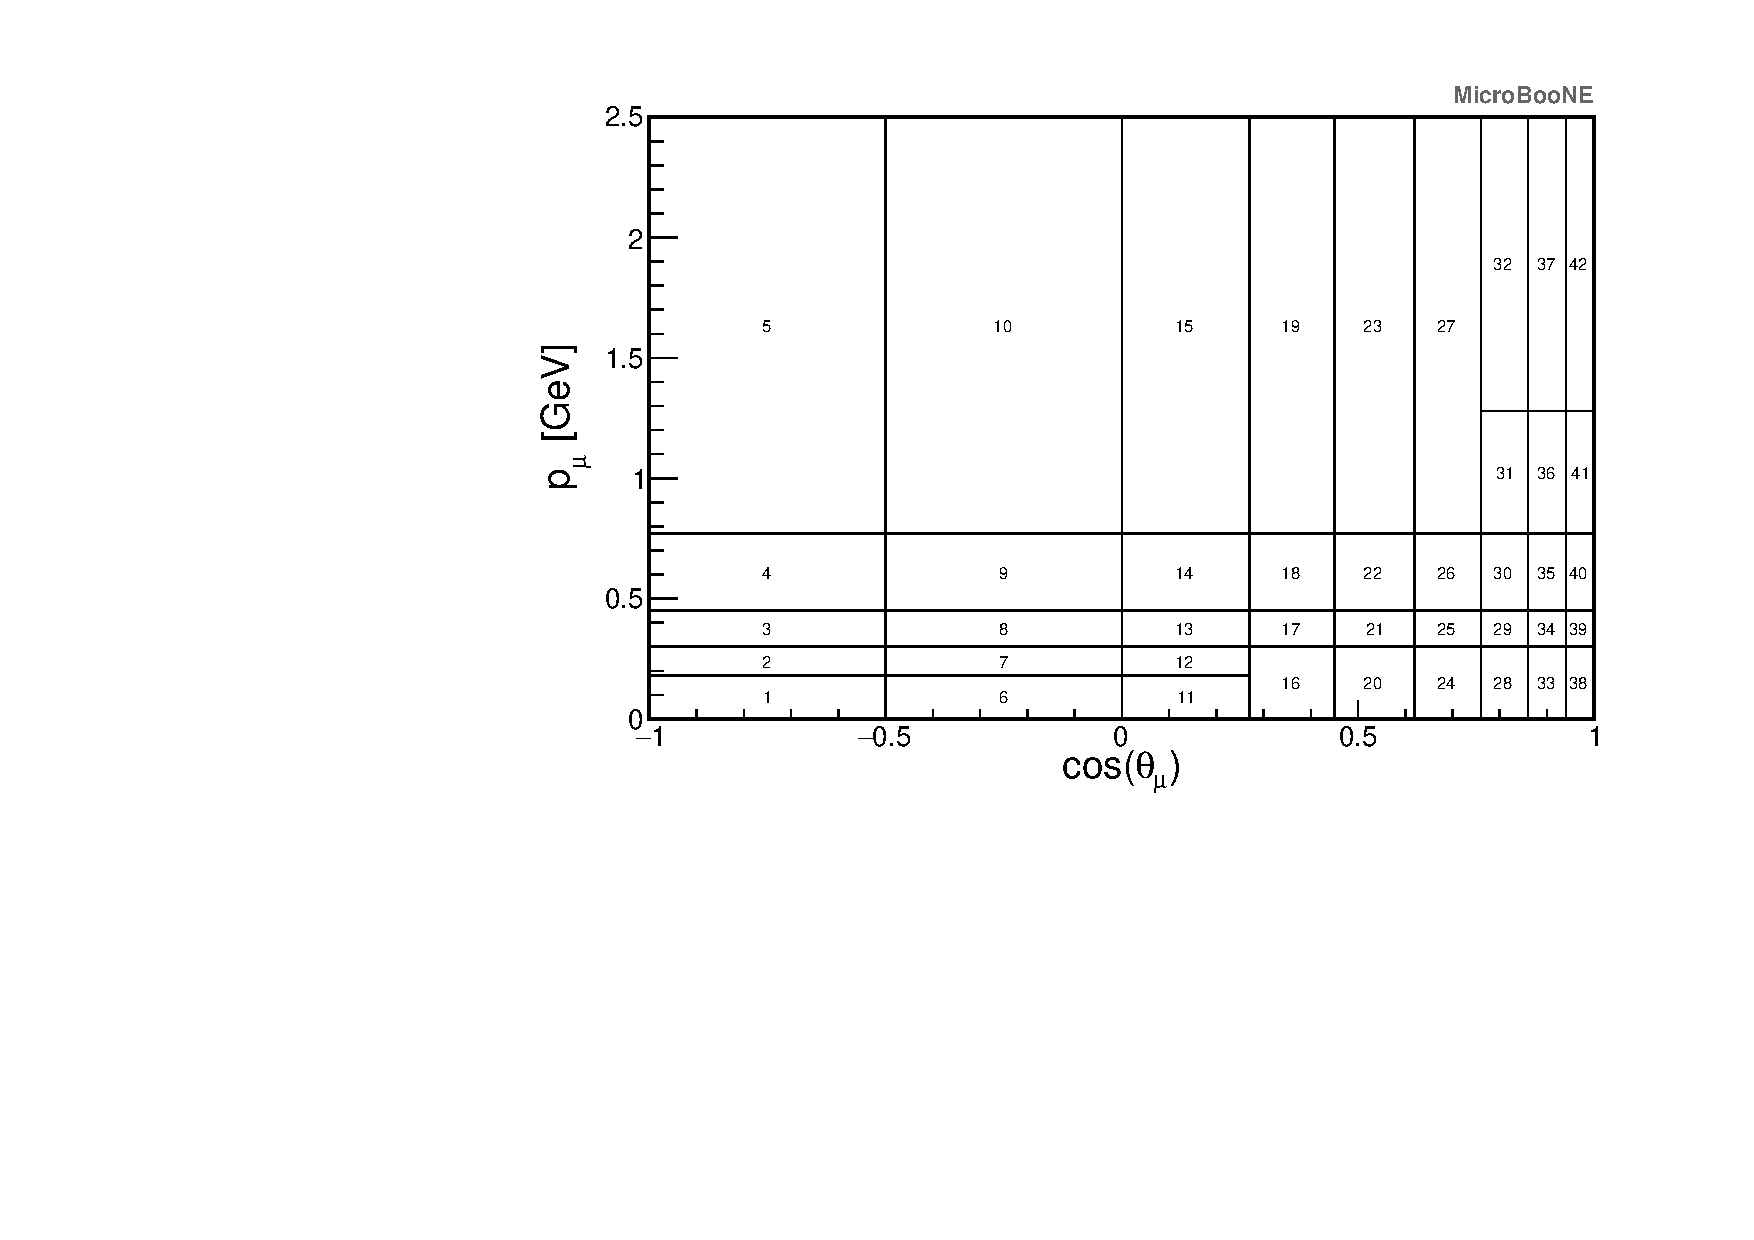
\includegraphics[width=.65\textwidth]{images/BinningPolyBin/bin_numbers}
%\caption{The figure shows the binning choice for the double-differential cross section in $p_\mu$ and $\cos\theta_\mu$. The numbers inside the bins show the bin ID, which is used to identify the bins in the following matrices.}
%\label{fig:polybins}
%\end{SCfigure}

\begin{figure}[]
\centering
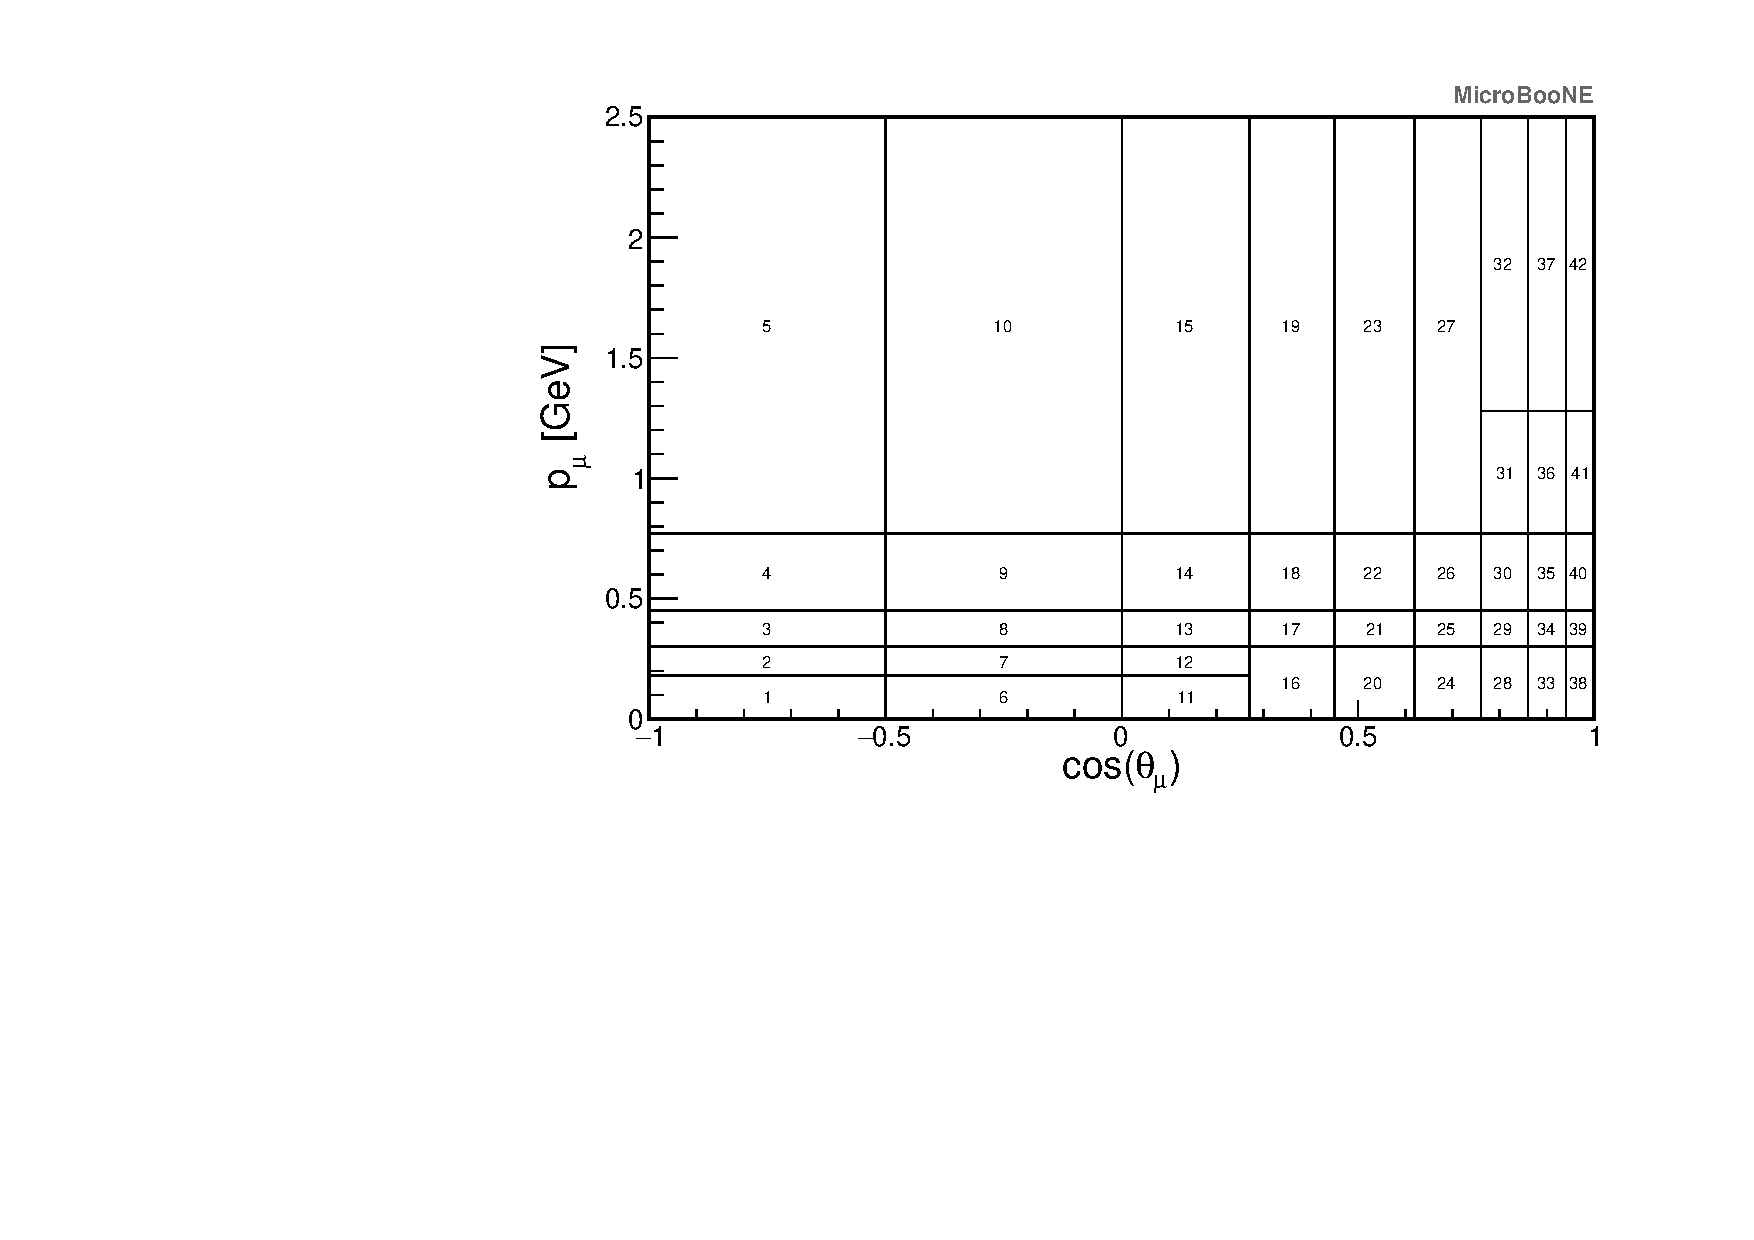
\includegraphics[width=.89\textwidth]{images/BinningPolyBin/bin_numbers}
\caption[Binning for the Double-Differential Cross Section]{The figure shows the binning choice for the double-differential cross section in $p_\mu$ and $\cos\theta_\mu$. The numbers inside the bins show the bin ID, which is used to identify the bins in the following matrices.}
\label{fig:polybins}
\end{figure}







\section{Total Cross Section}
\label{sec:total_xsec}

The total cross section can be calculated according to Equation~\ref{eq:xsec_total} and the quantities needed for this calculation are summarised in Table~\ref{tab:xsec_general_values} and \ref{tab:xsec_event_numbers}.
%
\begin{table}[]
\caption[Parameters Used for the Cross Section Extraction]{Parameters used for the flux integrated cross-section calculation. The integrated flux corresponds to an exposure of $1.592 \times 10^{20}$ \acrshort{pot}. The uncertainties on the flux and the number of targets will be discussed in the next chapter.}
\label{tab:xsec_general_values}
\centering
\begin{tabular}{ccc}
\toprule
Name & Variable & Value \\
\midrule
$\nu_\mu$ \acrshort{bnb} Flux      & $\Phi_{\nu_\mu}$           & $1.16859 \times 10^{11} \, \text{cm}^{-2}$ \\
Number of Targets Data  & $T^\text{data}$   & $2.6124^{+0.0036}_{-0.0003} \times 10^{31}$ \\
Number of Targets \acrshort{mc}    & $T^\text{\acrshort{mc}}$     & $2.6347 \times 10^{31}$ \\
Efficiency              & $\epsilon$                 & $0.57173 \pm 0.00082 \, (\text{stat.})$ \\
\bottomrule
\end{tabular}
\end{table}
%
\begin{table}[]
\caption[Total Number of Signal and Background Events]{Number of events used to calculate the flux integrated cross section. The numbers correspond to an exposure of $1.592 \times 10^{20}$ \acrshort{pot}.}
\label{tab:xsec_event_numbers}
\centering
\begin{tabular}{ccc}
\toprule
Name                   & Variable & Event Number  \\
\midrule
Measured Event Number         & $N$      & $27197 \pm 164$    \\
\midrule
$\nu_\mu$ \acrshort{cc} Events           & $S$      & $15348 \pm 34$    \\
\midrule
Cosmic Only (from off-beam)   & -        & $8868 \pm 66$   \\
Cosmic in \acrshort{bnb} (from \acrshort{mc})       & -        & $1961 \pm 12$   \\
\acrshort{outfv} (from \acrshort{mc})               & -        & $2308 \pm 13$    \\
\acrshort{nc} (from \acrshort{mc})                  & -        & $488.5 \pm 6.0$    \\
$\nu_e$ and $\bar{\nu}_e$ (from \acrshort{mc}) & -  & $16.5 \pm 1.0$   \\
$\bar{\nu}_\mu$ (from \acrshort{mc})     & -        & $133.9\pm 3.2$   \\
Dirt (from \acrshort{mc})                & -        & $1322.1\pm 8.8$  \\
\midrule
Total Background              & $B$      & $15099 \pm 69$  \\
\bottomrule
\end{tabular}
\end{table}
%
With $N = 27197 \pm 164$ selected data events and $B = 15099 \pm 69$ estimated background events, the data extracted cross section per nucleon is
\begin{equation}
\label{eq:data_xsec}
\sigma(\nu_\mu + \text{Ar} \rightarrow \mu^- + X) = 0.693 \pm 0.010 \, (\text{stat.}) \times 10^{-38} \, \text{cm}^2.
\end{equation}
%while for Tune 3 we have $B = 14891.4 \pm 69$ (and also a different efficiency), which gives:
%\begin{equation}
%\sigma^{(3)} = 0.714 \pm 0.010 \, (\text{stat.}) \times 10^{-38} \, \text{cm}^2
%\end{equation}
The \acrshort{mc} cross section predicted by \g can be obtained by
\begin{equation}
\sigma_\text{\acrshort{mc}} = \frac{S}{\epsilon \cdot T^\text{MC} \cdot \Phi_{\nu_\mu}},
\end{equation}
where $S$ is the number of selected signal events, $S = 14657 \pm 51$, which gives
\begin{equation}
\sigma_\text{\acrshort{mc}} = 0.871 \pm 0.002 \, (\text{stat.}) \times 10^{-38} \, \text{cm}^2.
\end{equation}
%for Tune 1, and 
%\begin{equation}
%\sigma_\text{\acrshort{mc}}^{(3)} = 0.826 \pm 0.002 \, (\text{stat.}) \times 10^{-38} \, \text{cm}^2
%\end{equation}
%for Tune 3.
The percental difference between the two cross sections is $(\sigma - \sigma_\text{MC})/{\sigma_\text{MC}} =  -20.4\%$, 
which is covered by the total systematic uncertainty as will be shown in the next chapters.
%for Tune 1, and 
%\begin{equation}
%\frac{\sigma^{(3)} - \sigma_\text{\acrshort{mc}}^{(3)}}{\sigma_\text{\acrshort{mc}}^{(3)}} =  -13.6\%
%\end{equation}
%for Tune 3. 
%To remark, the Tune 1 cross section is evaluated with background and efficiency estimation from the Tune 1 simulation, while the Tune 3 cross section is estimated with background and efficiency estimation from the Tune 3 simulation. The data are the same for both. 
The total cross section from data and \acrshort{mc} is also shown in Figure~\ref{fig:total_xsec_pdg}. Note that the cross section is divided by the neutrino energy in this plot. The horizontal bars on the $x$ axis come from the width of the neutrino energy spectrum, shown in Section~\ref{sec:flux}.




\begin{figure}[t]
\centering
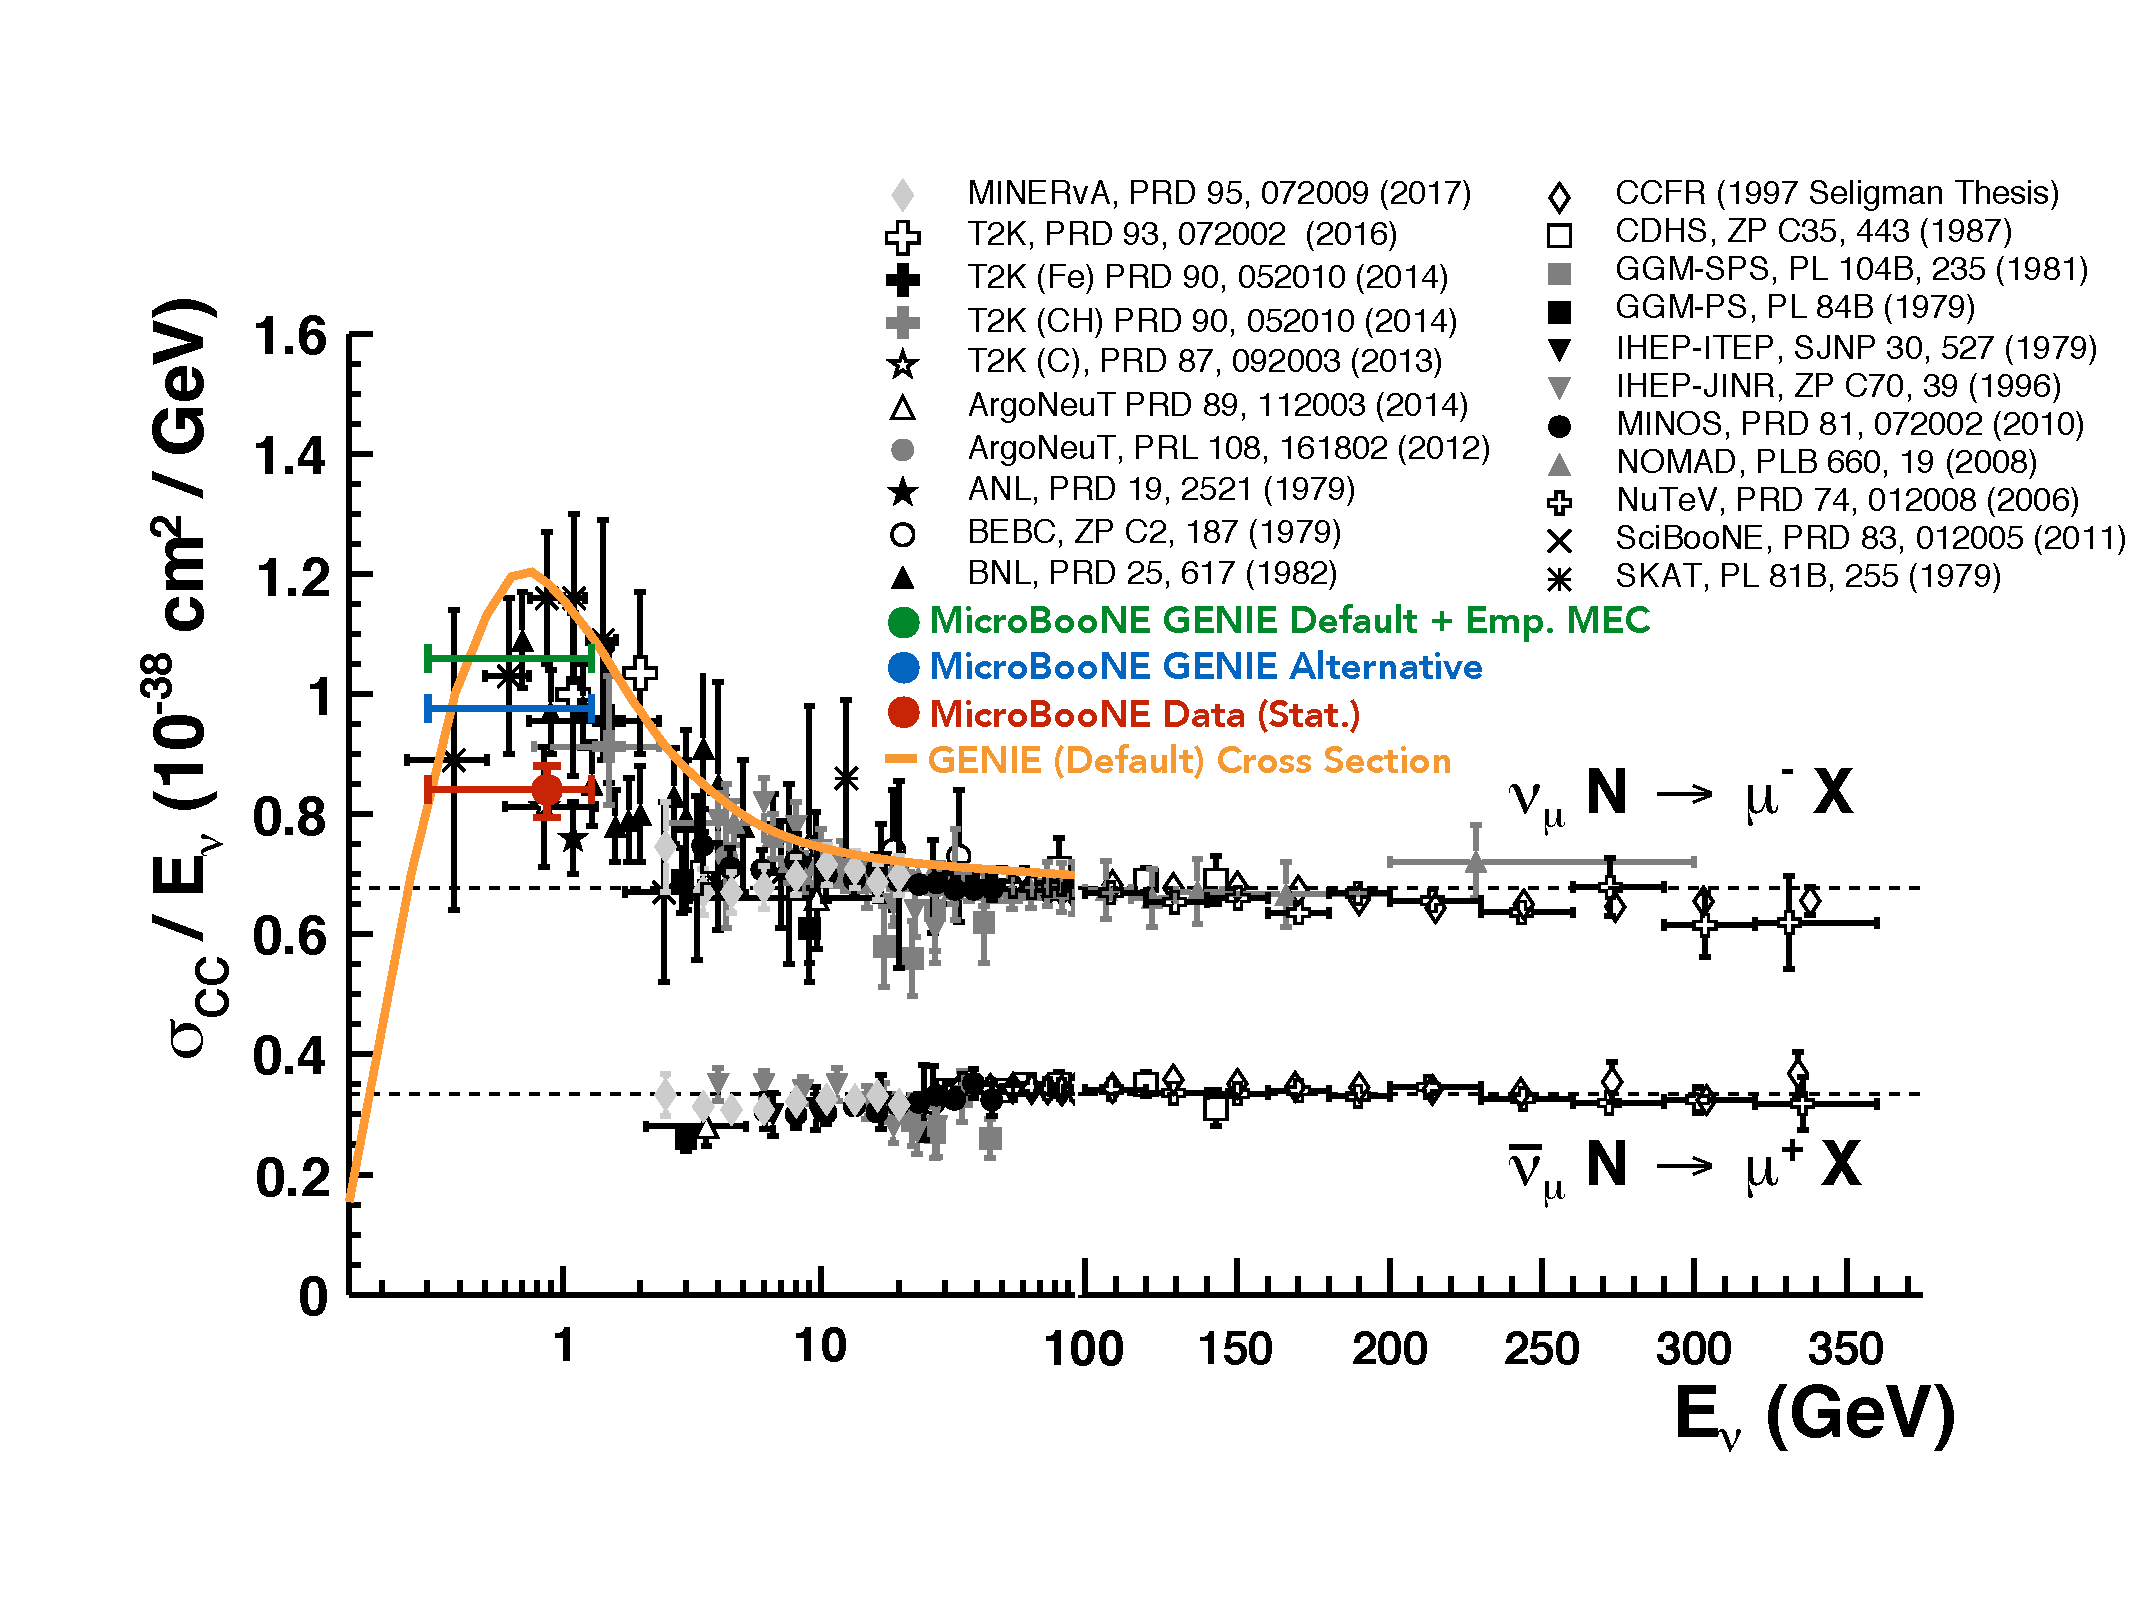
\includegraphics[width=.95\textwidth]{images/total_xsec_pdg_2}
\caption[Total Cross Section Compared to Different Experiments]{\acrshort{cc} inclusive measurements for $\nu_\mu$ and $\bar{\nu}_\mu$ from different experiments with different nuclear targets in black and grey. The green and blue points show the \acrshort{mc} predicted cross section by the \g default and alternative configurations, respectively. The red point shows the data extracted cross section from the analysis presented in this thesis. Only statistical uncertainties are shown. The orange curve shows the \g default initial cross section as a function of neutrino energy.}
\label{fig:total_xsec_pdg}
\end{figure}


%**********************************************************

\section[Cross Section: Muon Momentum]{Differential Cross Section in Muon Momentum}
\label{sec:mumom_xsec}

This section presents the calculation of the single differential cross section in muon momentum $p_\mu$. The cross section is calculated according to Equation~\eqref{eq:xsec_differential} and the number of events per bin is shown in Table~\ref{tab:pmu_events}.

%\subsection{Background Subtraction for $p_\mu$}
%
%The next step towards the differential cross section measurement is to perform the background subtraction for the selected event distributions shown in Figure~\ref{fig:trkmom} and~\ref{fig:trkcostheta}. The distributions before and after background subtraction for the momentum are shown in Figure~\ref{fig:trkmom_bkg_sub}. All the backgrounds have been subtracted from both the \acrshort{mc} and the data events: cosmics from off-beam data, cosmics that overlay neutrino interactions, out of \acrshort{fv} events, neutral current events, $\bar{\nu}_\mu$ and $\overset{\text{\relsize{-1}(}-\text{\relsize{-1})}}{\nu}_e$ events. The statistical uncertainties have been propagated.

%\begin{figure}[t]
%\centering
%\subfloat[][]
%   {\includegraphics[width=.45\textwidth]{images/XSecPmu/trkmom_selectedevents}
%   \label{fig:trkmom_selectedevents}} \quad
%\subfloat[][]
%   {\includegraphics[width=.45\textwidth]{images/XSecPmu/trkmom_selectedevents_bkgsubtracted}
%   \label{fig:trkmom_selectedevents}} \quad
%\caption{The left plot shows the distribution of selected events, while the right plot shows the same distribution after background subtraction. The entries per bin have not been divided by the bin width. The data error bars show the statical uncertainty only. The \acrshort{mc} used for these plots is Tune 1.}
%\label{fig:trkmom_bkg_sub}
%\end{figure}

%\begin{landscape}
\begin{table}[]
\scriptsize
\begin{adjustwidth}{-1.5cm}{-1cm}
\caption[Selected Events Per $p_\mu$ Bin]{The table shows the number of selected events per $p_\mu$ reconstructed bin and different categories. Only statistical uncertainties  are shown.}
\label{tab:pmu_events}
\centering
\begin{tabular}{c|cc|ccccccc}
\toprule
    & \multicolumn{2}{c}{Data}    & \multicolumn{6}{c}{\acrshort{mc}} \\
Bin & Selected & Cosmic & $\nu_\mu$ \acrshort{cc} & Cosmic  & \acrshort{outfv} & DIRT & \acrshort{nc} & $\nu_e$ and $\bar{\nu}_e$ & $\bar{\nu}_\mu$ \\
    & Events   & Only   & Signal       & in \acrshort{bnb}  &       &      &    &                           &                 \\
\midrule
1 & 728 $\pm$ 26 & 374 $\pm$ 13 & 201.8 $\pm$ 3.8 & 80.1 $\pm$ 2.4 & 77.3 $\pm$ 2.3    & 65.1 $\pm$ 1.9 & 77.9 $\pm$ 2.4    & 2.40 $\pm$ 0.37 & 1.54 $\pm$ 0.33 \\ 
2 & 4213 $\pm$ 64 & 1748 $\pm$ 29 & 1786 $\pm$ 11 & 286.7 $\pm$ 4.6 & 480.9 $\pm$ 5.9  & 293.5 $\pm$ 4.1 & 184.1 $\pm$ 3.6 & 5.0 $\pm$ 0.55 & 12.41 $\pm$ 0.96 \\ 
3 & 6670 $\pm$ 81 & 2303 $\pm$ 33 & 3193 $\pm$ 15 & 336.0 $\pm$ 4.9 & 636.8 $\pm$ 6.8  & 347.4 $\pm$ 4.4 & 126.0 $\pm$ 3.0 & 4.49 $\pm$ 0.52 & 21.1 $\pm$ 1.2 \\ 
4 & 8126 $\pm$ 90 & 1853 $\pm$ 30 & 5241 $\pm$ 19 & 381.4 $\pm$ 5.3 & 633.3 $\pm$ 6.8  & 250.1 $\pm$ 3.8 & 61.2 $\pm$ 2.1  & 2.83 $\pm$ 0.44 & 39.3 $\pm$ 1.7 \\ 
5 & 5351 $\pm$ 73 & 1496 $\pm$ 27 & 3758 $\pm$ 16 & 506.9 $\pm$ 6.1 & 352.9 $\pm$ 5.1  & 121.9 $\pm$ 2.6 & 25.5 $\pm$ 1.4  & 1.18 $\pm$ 0.28 & 42.4 $\pm$ 1.8 \\ 
6 & 1905 $\pm$ 43 & 944 $\pm$ 21 & 1101.0 $\pm$ 8.9 & 313.4 $\pm$ 4.8 & 113.5 $\pm$ 2.8  & 122.1 $\pm$ 2.6 & 10.9 $\pm$ 0.8 & 0.61 $\pm$ 0.20 & 16.72 $\pm$ 1.2 \\ 
\bottomrule
\end{tabular}
\end{adjustwidth}
\end{table}
%\end{landscape}



%\subsection{Migration Matrix for $p_\mu$}
%\label{sec:migration_pmu}

The simulated distributions must be smeared in order to calculate the efficiency as a function of reconstructed muon momentum, using Equation~\eqref{eq:eff_smear}. The migration matrix was estimated from simulation and is found to be
%\begin{adjustwidth}{-1cm}{-1cm}
\begin{equation}
S_{ij} =
\begin{bmatrix}
0.210  &  0.0546  &  0.00343  &  0.00133  &  0.000822  &  0.000555  &  0.000442  &   \\
0.467  &  0.640  &  0.130  &  0.0141  &  0.00593  &  0.00324  &  0.00434  &   \\
0.190  &  0.247  &  0.671  &  0.134  &  0.0219  &  0.0152  &  0.0201  &   \\
0.0739  &  0.0380  &  0.175  &  0.723  &  0.222  &  0.0818  &  0.0867  &   \\
0.0390  &  0.0122  &  0.014  &  0.116  &  0.660  &  0.357  &  0.214  &   \\
0.0161  &  0.00655  &  0.00524  &  0.00923  &  0.0856  &  0.522  &  0.539  &   \\
0.0039  &  0.00134  &  0.00104  &  0.00139  &  0.00345  &  0.0202  &  0.135  &   \\
\end{bmatrix}.
\end{equation}
The migration matrix is also illustrated in Figure~\ref{fig:trkmom_migration_matrix_2d}. Note that entries $i = 7, \forall j$ and $j = 7, \forall i$ show the overflow values (muon momentum above 2.5 GeV).

\begin{figure}[]
\centering
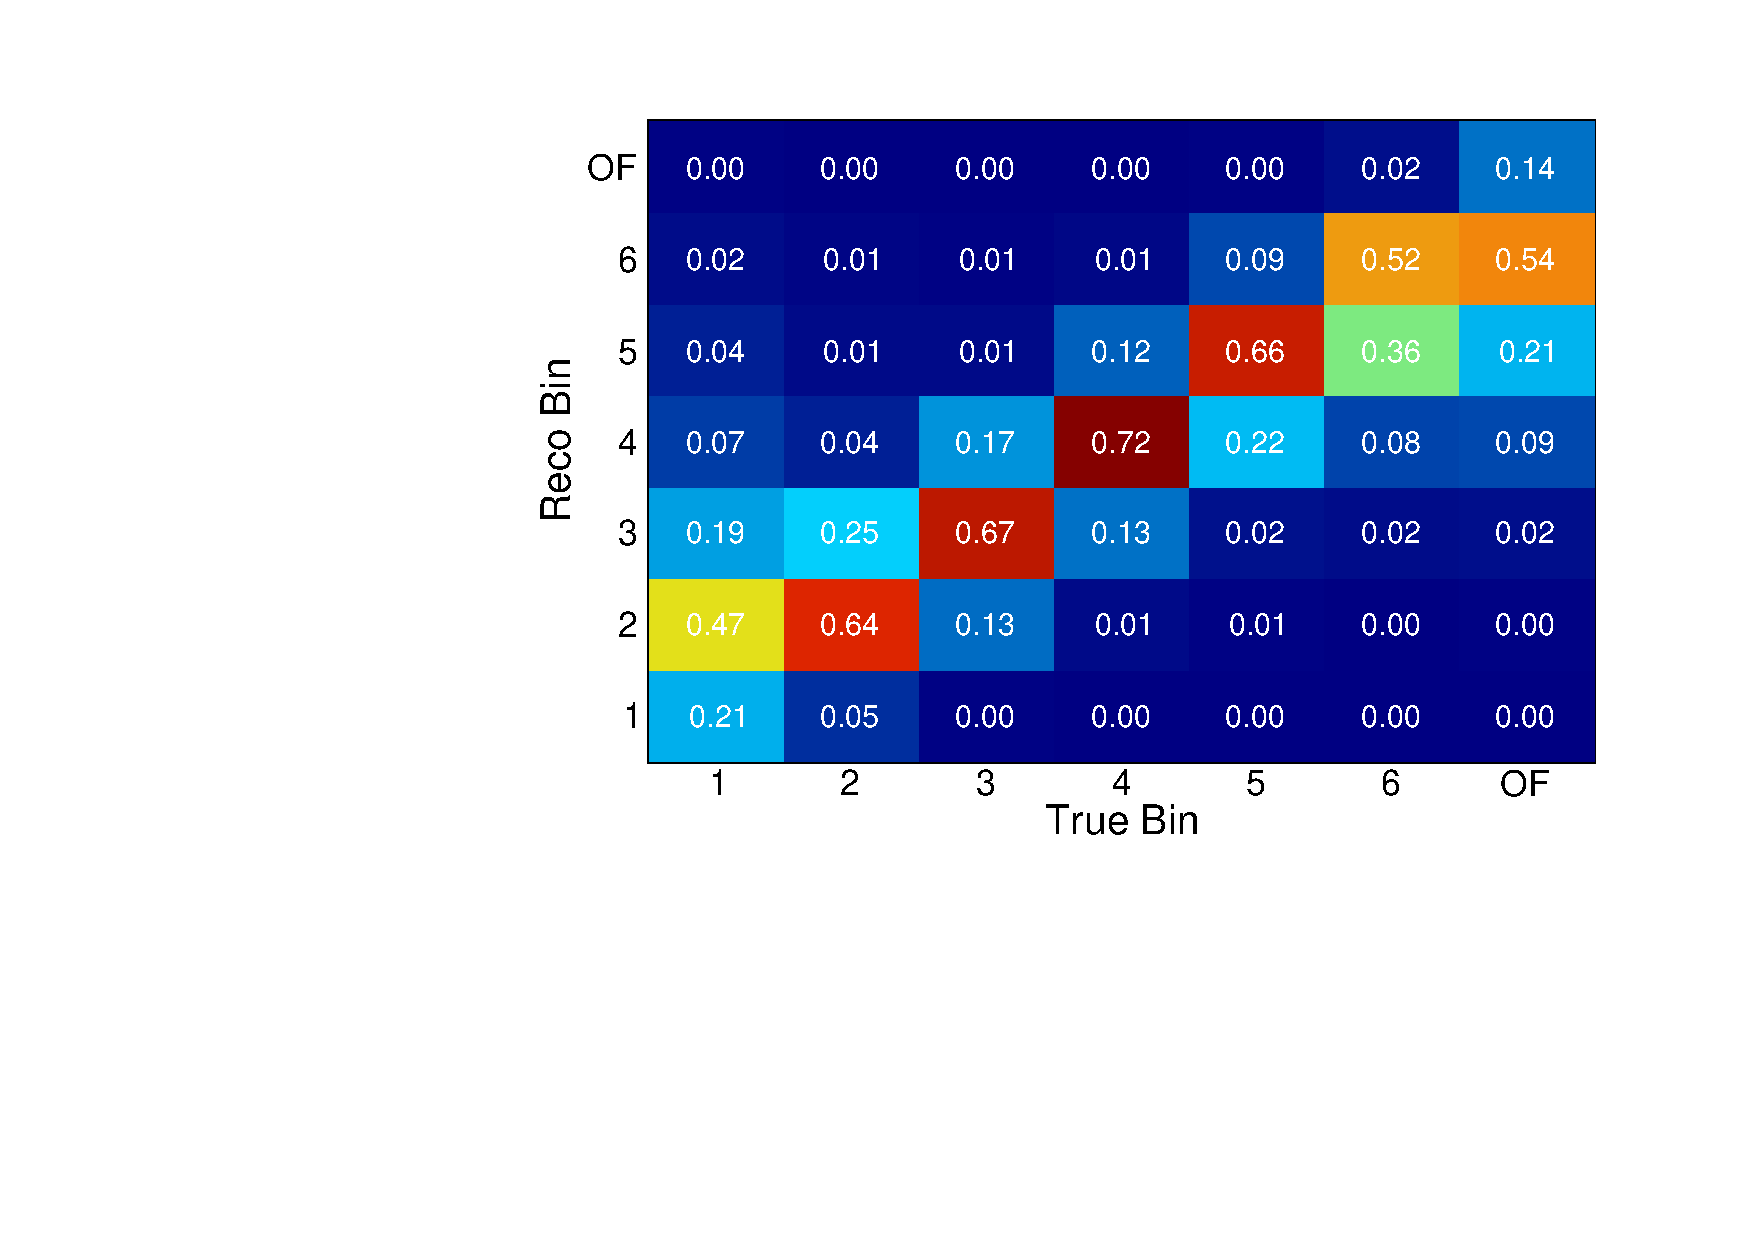
\includegraphics[width=.80\textwidth]{images/XSecPmu/migration_matrix_2d}
\caption[Smearing Matrix for the $p_\mu$ Distributions]{Smearing matrix for the $p_\mu$ distributions. It shows the probability that an event in a true bin is observed in a reconstructed bin. ``OF'' shows the overflow bin (muon momentum above 2.5 GeV).}
\label{fig:trkmom_migration_matrix_2d}
\end{figure}




Figure~\ref{fig:trkmom_all_selected} shows the distribution of the true muon momentum for all generated muons from $\nu_{\mu}$ \acrshort{cc} interactions in the \acrshort{fv} and for selected events. The ratio of these two distributions is shown in Figure~\ref{fig:trkmomefficiecy_mumon_true}, which corresponds the efficiency as a function of the true muon momentum. This is the same as the one shown in the previous chapter, but now with the final binning. 

On the right side of Figure~\ref{fig:trkmom_eff_smear}, the smeared distributions for both the selected and generated events (\ref{fig:trkmom_all_selected_smear}), and the new efficiency $\tilde{\epsilon}$ as a function of the reconstructed muon momentum (\ref{fig:trkmom_efficiecy_reco}) are shown. This efficiency will be used for the cross-section calculation.

\begin{figure}[t]
\centering
\subfloat[][Before smearing.]
   {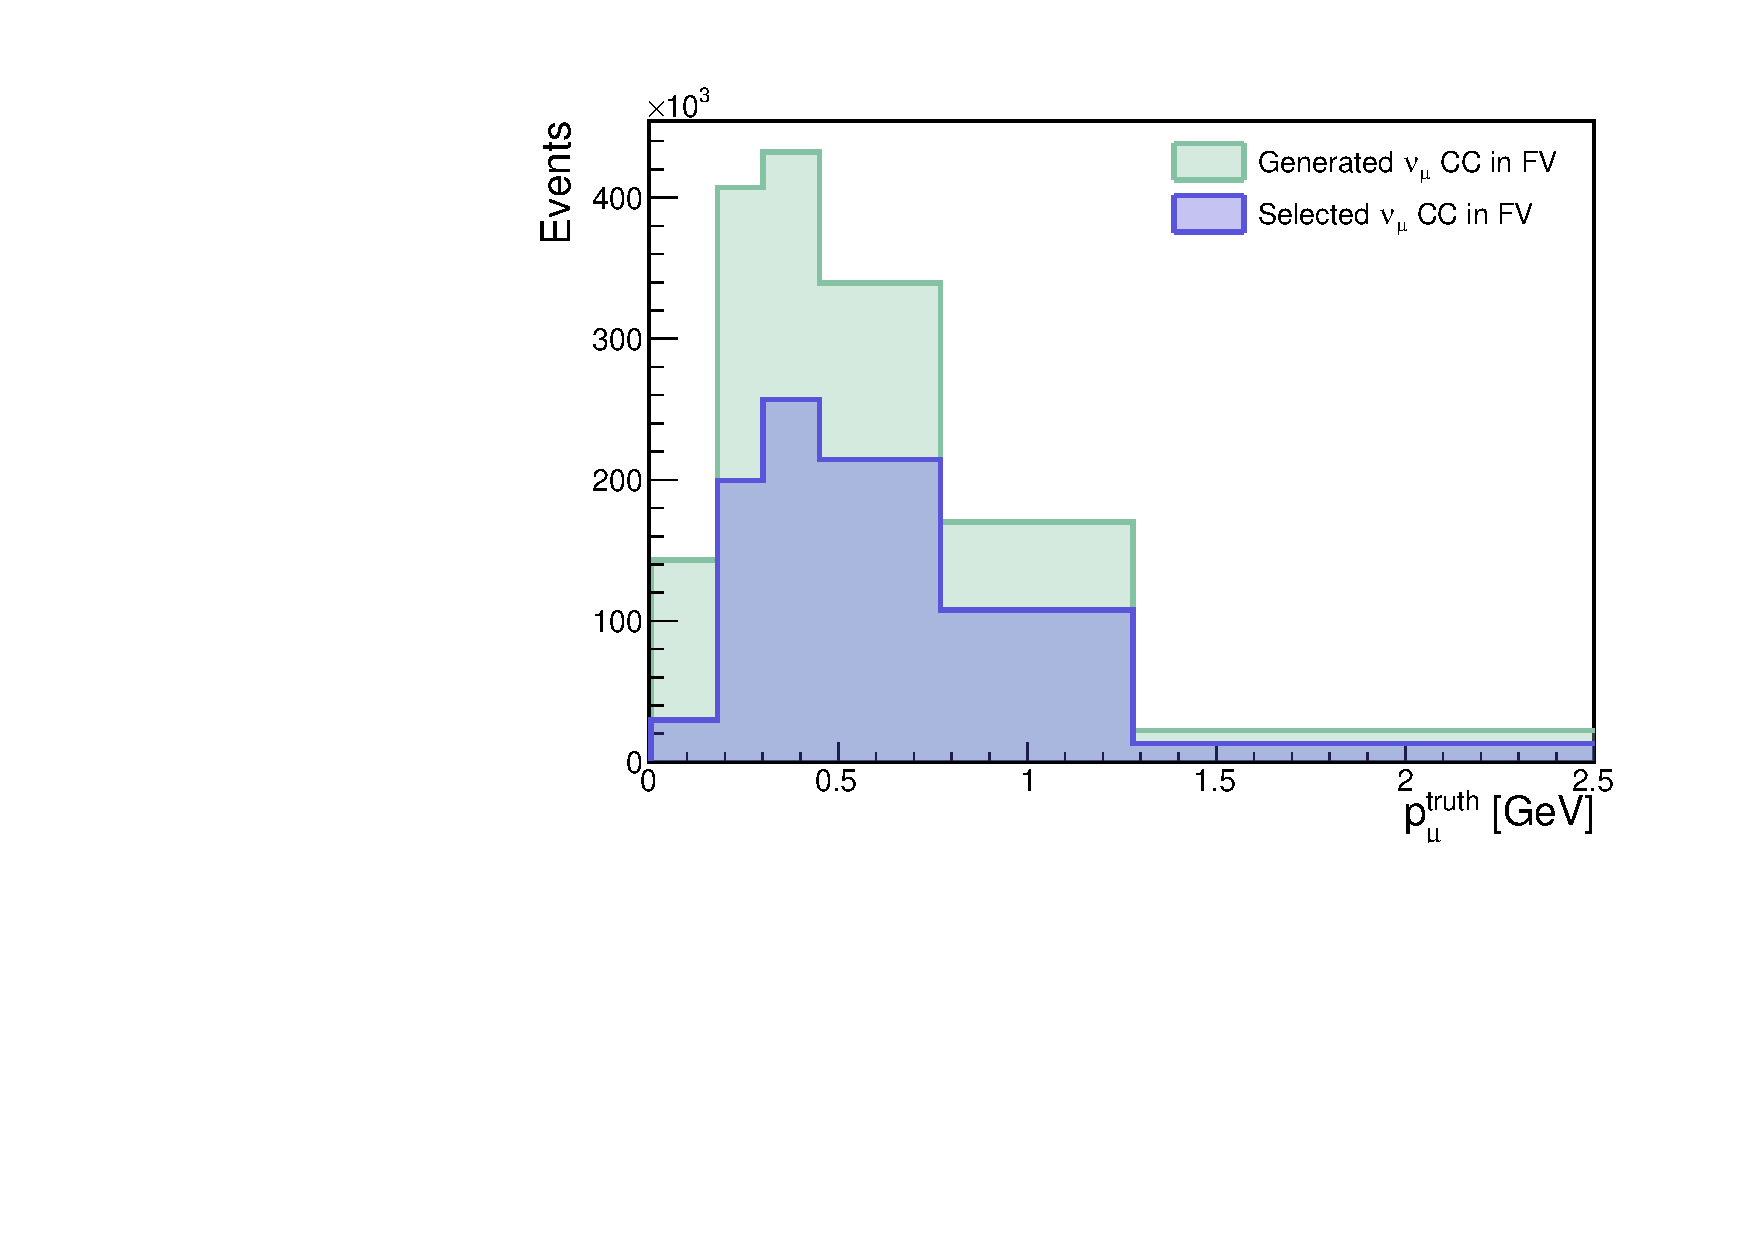
\includegraphics[width=.5\textwidth]{images/XSecPmu/trkmomall_selected}
   \label{fig:trkmom_all_selected}} 
\subfloat[][After smearing.]
   {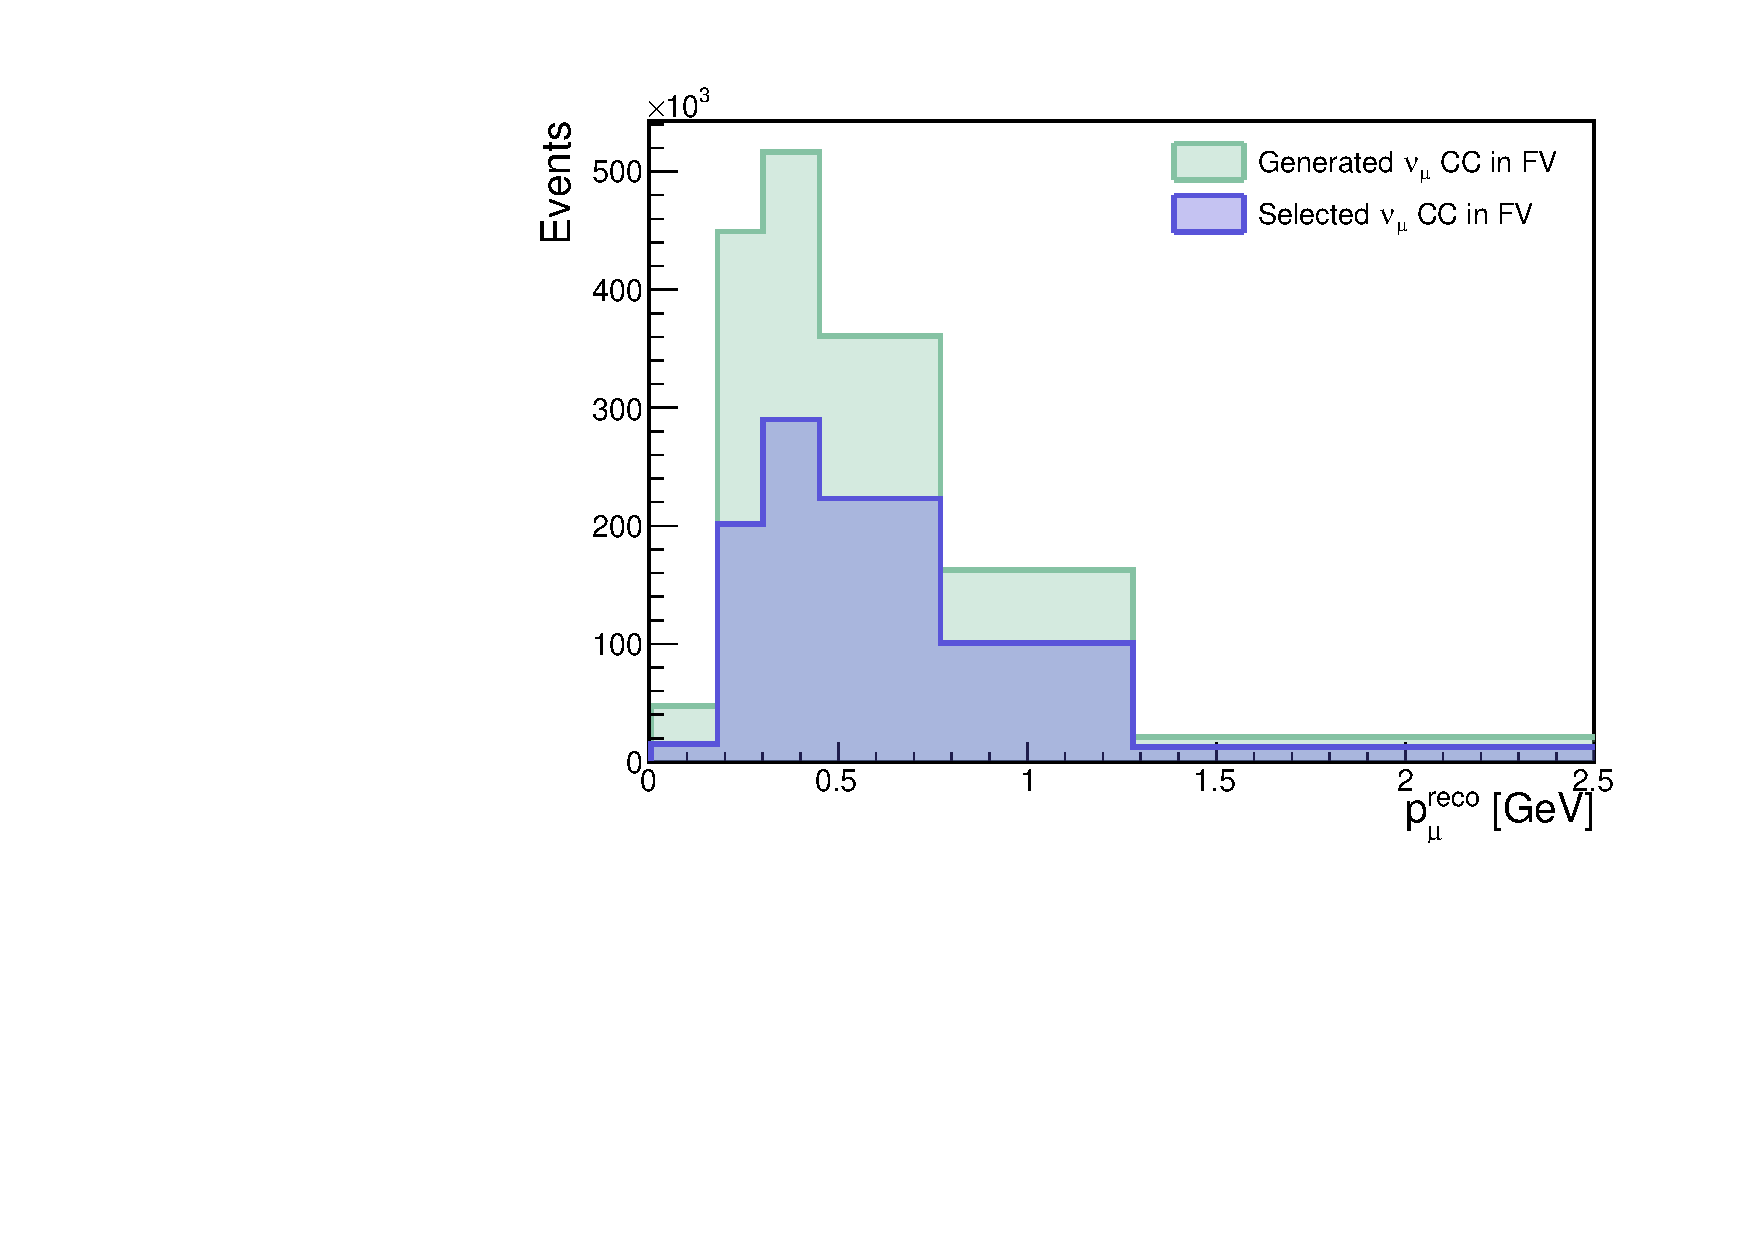
\includegraphics[width=.5\textwidth]{images/XSecPmu/trkmom_all_selected_smear}
   \label{fig:trkmom_all_selected_smear}} \\
\subfloat[][Before smearing.]
   {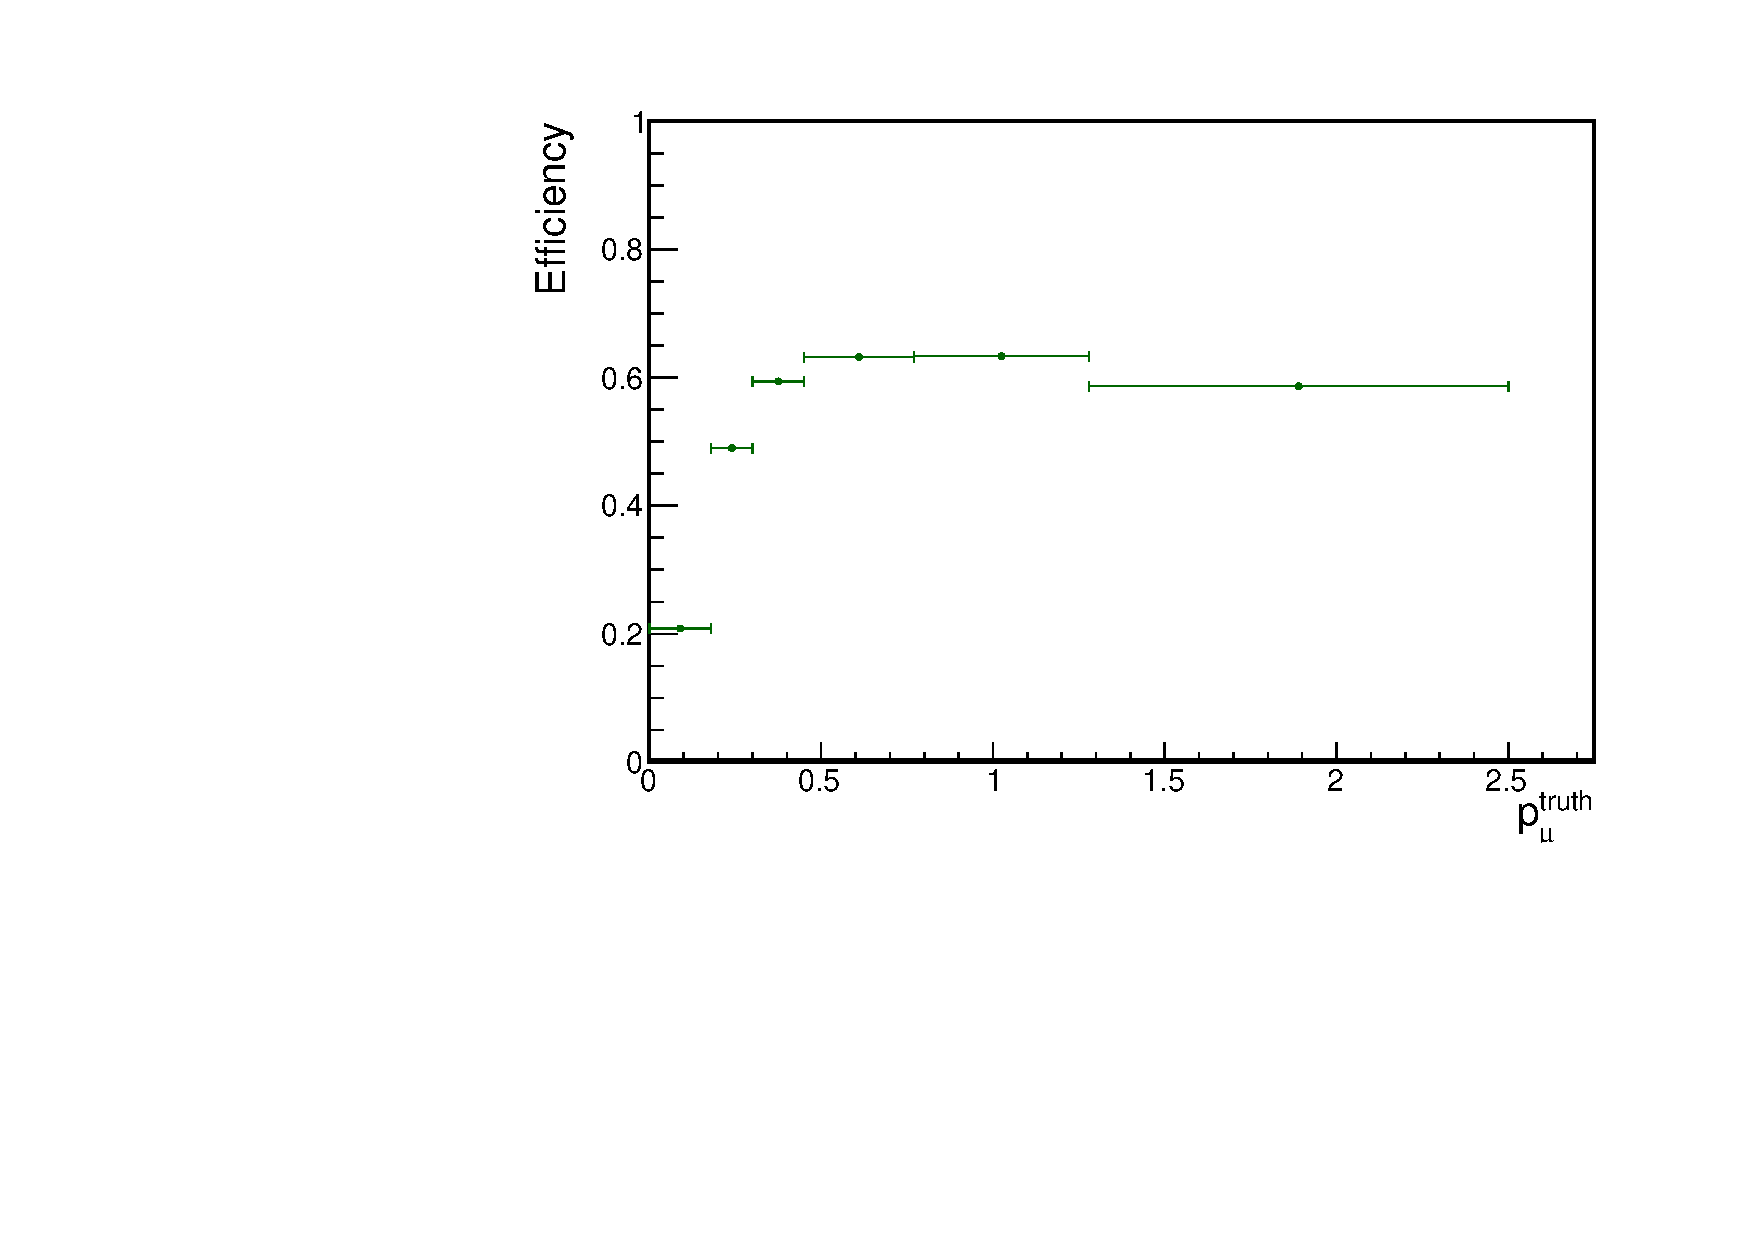
\includegraphics[width=.5\textwidth]{images/XSecPmu/trkmomefficiecy_mumon_true}
   \label{fig:trkmomefficiecy_mumon_true}} 
\subfloat[][After smearing.]
   {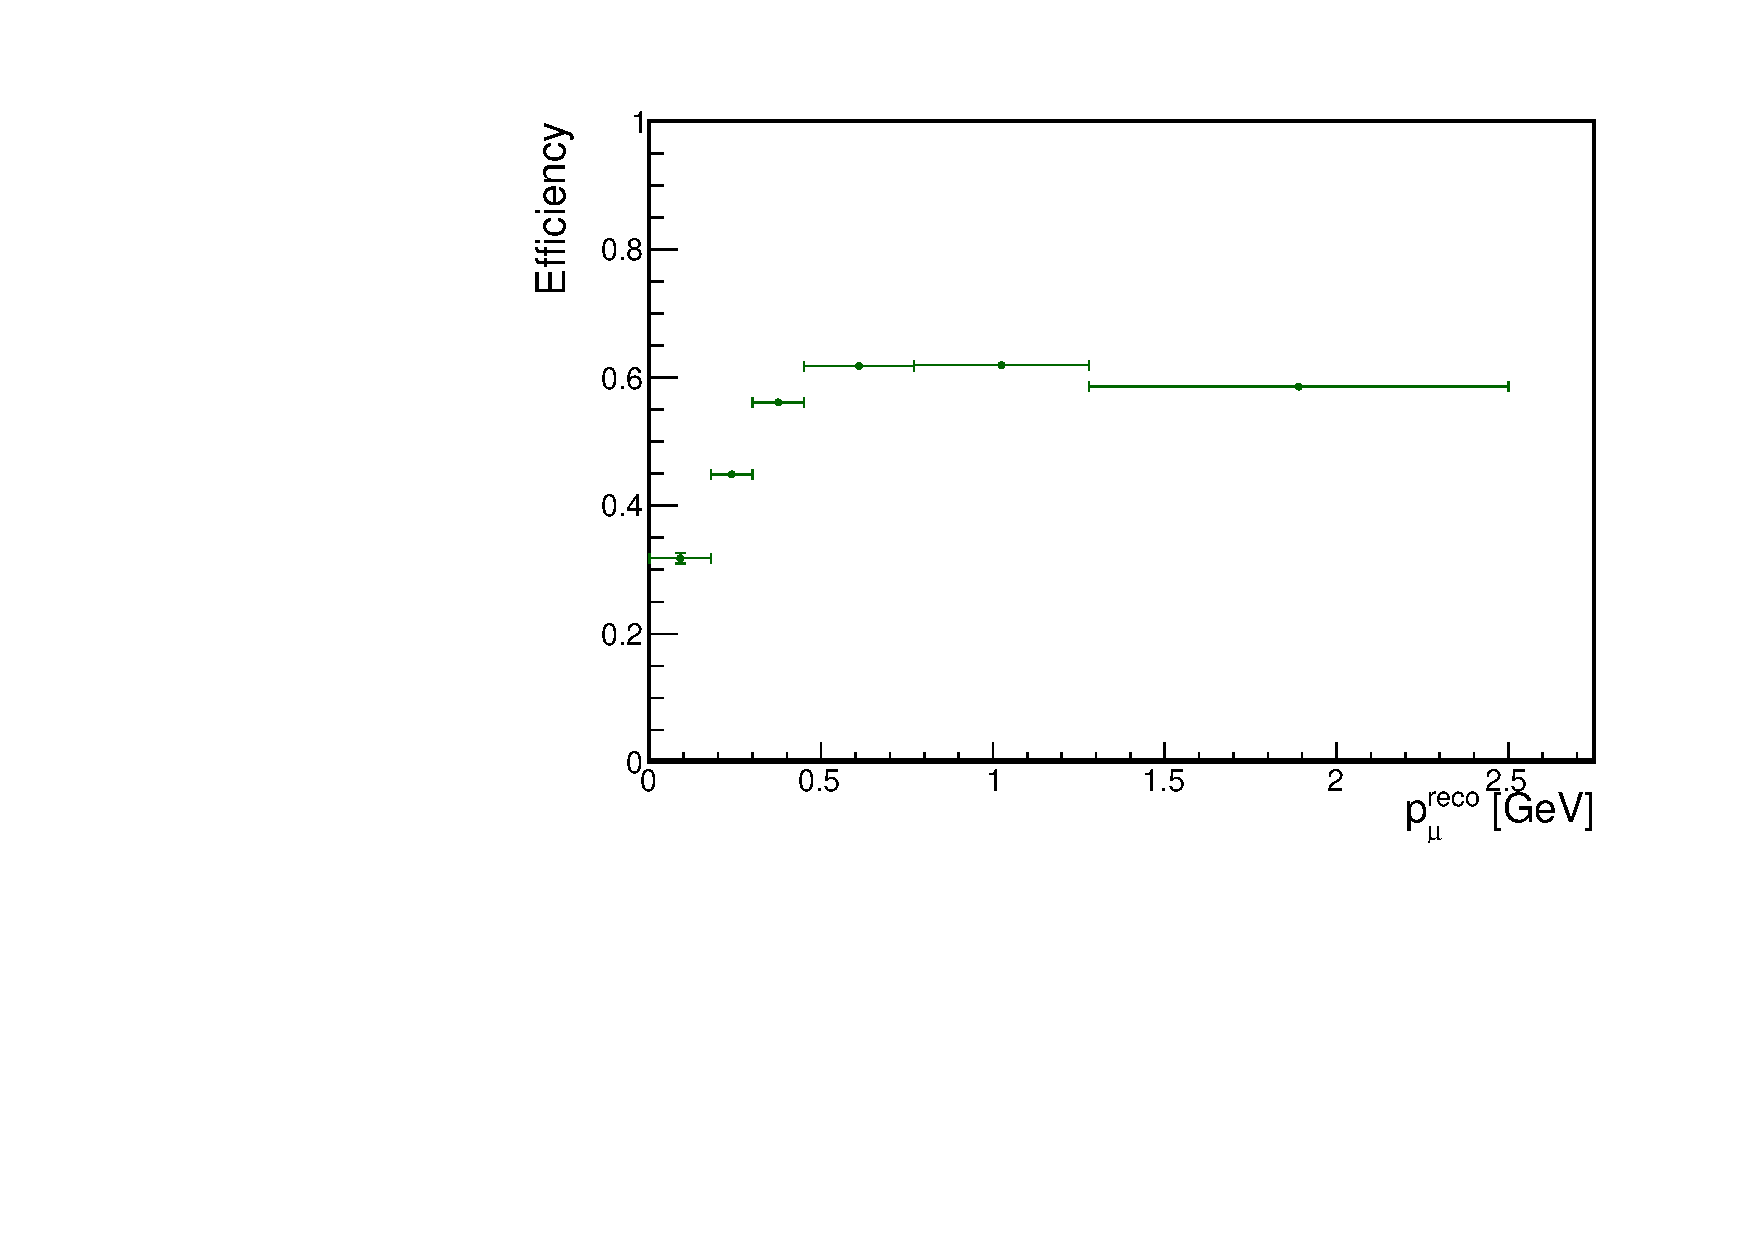
\includegraphics[width=.5\textwidth]{images/XSecPmu/trkmom_efficiecy_reco}
   \label{fig:trkmom_efficiecy_reco}} \\
\caption[Simulated $p_\mu$ Distributions and Efficiency in $p_\mu$ Bins]{Top: distributions of the generated (green) and selected (blue) signal events in terms of the simulated variable $p_\mu^\text{truth}$~\protect\subref{fig:trkmom_all_selected} and, after smearing, in terms of the reconstructed variable $p_\mu^\text{reco}$~\protect\subref{fig:trkmom_all_selected_smear}. Bottom: ratio of the distributions above, meaning the efficiency in $p_\mu^\text{truth}$~\protect\subref{fig:trkmomefficiecy_mumon_true} and in $p_\mu^\text{reco}$~\protect\subref{fig:trkmom_efficiecy_reco}.}
\label{fig:trkmom_eff_smear}
\end{figure}

%The statistical uncertainties on the efficiency (not visible in the plots) have been calculated using the equation:
%\begin{equation}
%\sigma_{\epsilon_i} = \frac{1}{\sqrt{N_i}} \sqrt{\frac{n_i}{N_i}\left(1-\frac{n_i}{N_i}\right)}
%\end{equation}
%where $n_i$ and $N_i$ are the selected and generated events in bin $i$ respectively. This formula comes from a binomial distribution with probability $\epsilon$ and $N$ trials. It holds in our case as the efficiency is never close to either 0, or 1. In our case $N$ has been generated by our \acrshort{mc} and is large enough to guarantee that the efficiency follows a Gaussian distribution with the \acrshort{std} shown above. The statistical uncertainties on the efficiency will be negligible though compared to the data statistical uncertainties and systematic uncertainties.
%Note, however, that \acrshort{mc} statistical uncertainties for the cross-section measurement are evaluated through reweighing the \acrshort{mc} events. This is described in details in Section~\ref{sec:error_mcstat}.


%\subsection{Cross-Section Central Values}

Putting all the quantities calculated in the previous sections into Equation~\eqref{eq:xsec_differential}, the $\nu_\mu$ \acrshort{cc} inclusive differential cross section on argon as a function of muon momentum is extracted and shown in Figure~\ref{fig:trkmom_xsec}. 
%The green distributions show the cross section according to the \acrshort{mc} and the light green error bands represent the statistical uncertainty on the \acrshort{mc}. The black data points show the data extracted cross section. The error bars represent the data statistical uncertainties including  the statistical uncertainties on the \acrshort{mc} estimated backgrounds and efficiency.
\begin{figure}[t]
\centering
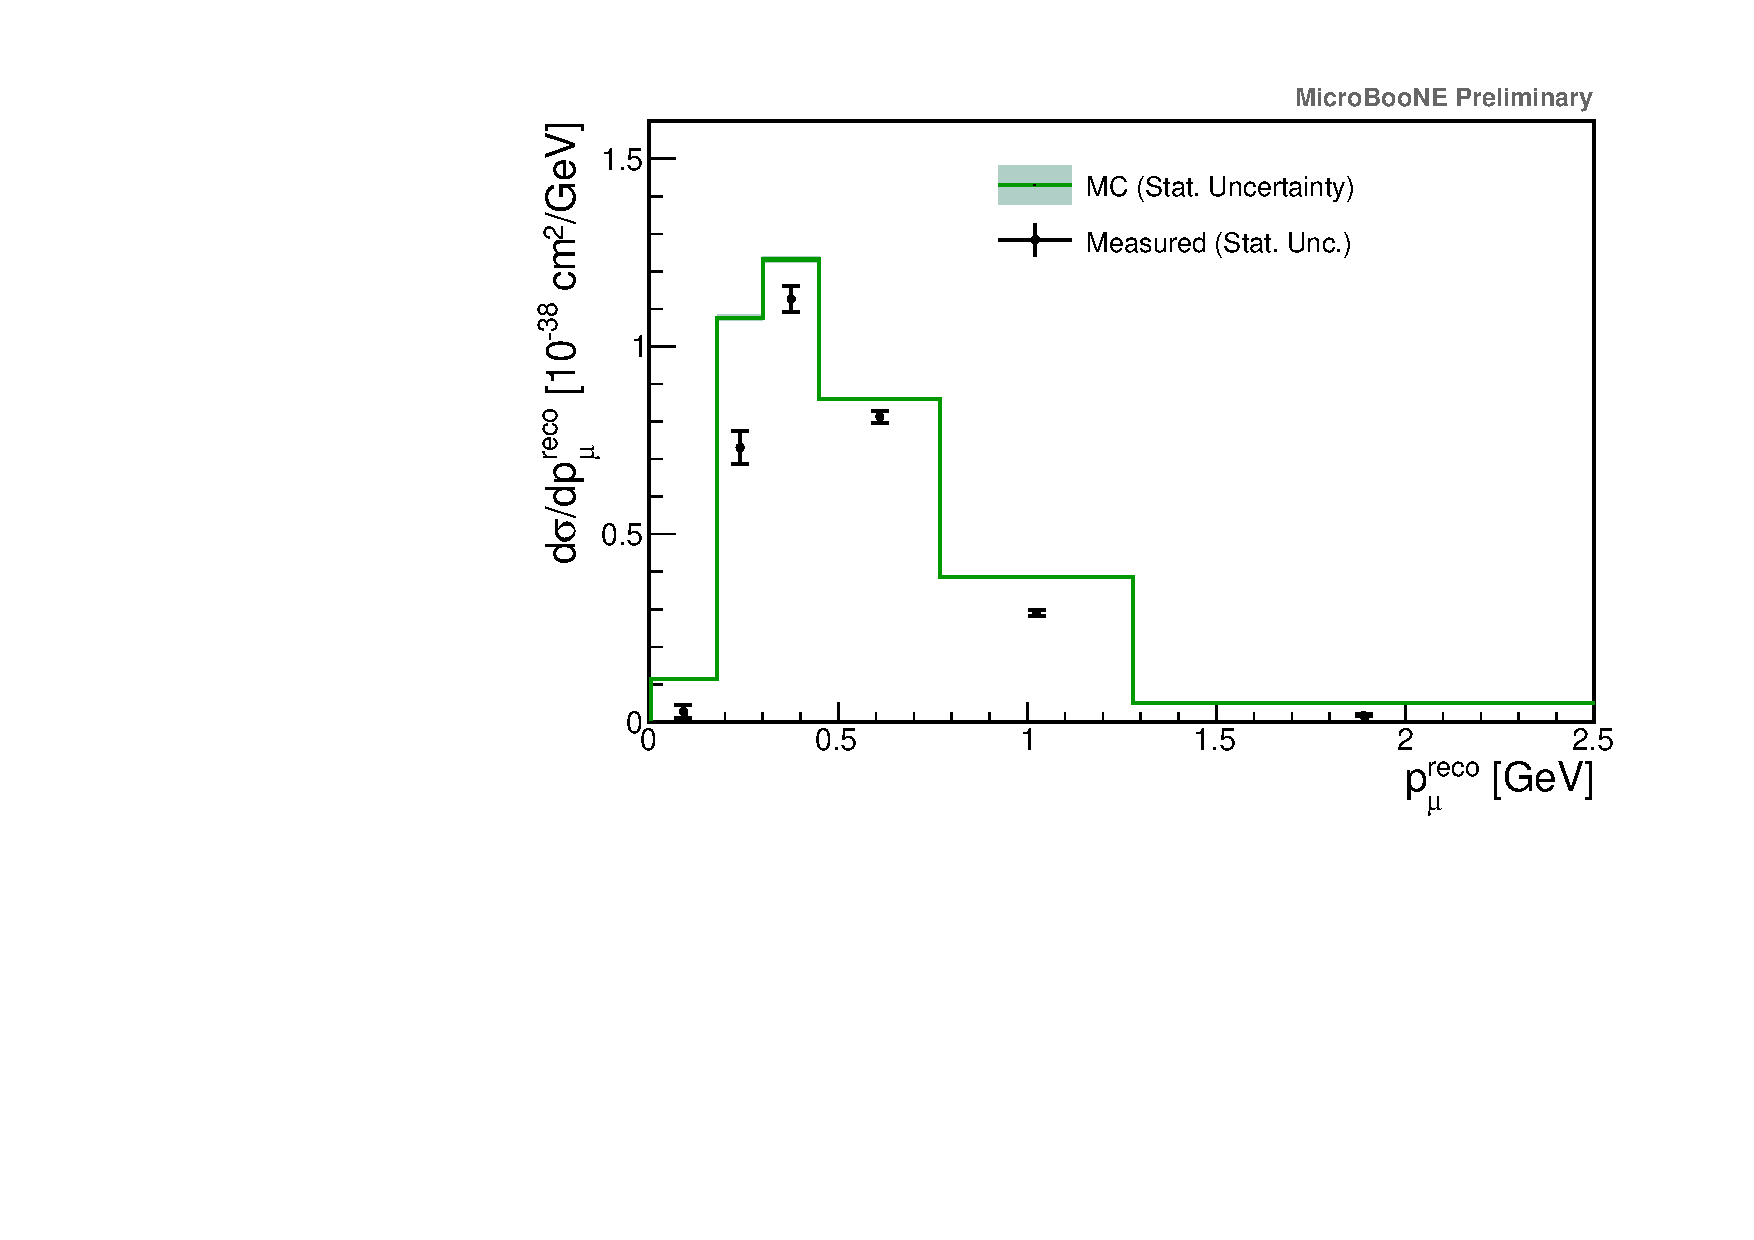
\includegraphics[width=.80\textwidth]{images/XSecPmu/trkmom_xsec}
\caption[$d\sigma/dp_\mu$ Single Differential Cross Section (Stat. Unc. Only)]{$\nu_\mu$ \acrshort{cc} inclusive differential cross section on argon per nucleon as a function of the reconstructed muon momentum. The black data points show the data extracted cross section, while the green curve shows the \acrshort{mc} predicted cross section. The data error bars and the \acrshort{mc} error bands show statistical uncertainties only. Systematic uncertainties are treated in Chapter~\ref{ch:systematics}.}
\label{fig:trkmom_xsec}
\end{figure}



\clearpage
%**********************************************************
\section[Cross Section: Muon Angle]{Differential Cross Section in Muon Angle}
\label{sec:muangle_xsec}

This section presents the calculation of the single differential cross section in muon angle $\cos\theta_\mu$. The cross section is calculated according to Equation~\eqref{eq:xsec_differential} and the number of events per bin is shown in Table~\ref{tab:costhetamu_events}.





%\subsection{Background Subtraction for $\cos(\theta_\mu)$}

%The next step towards the differential cross section measurement is to perform the background subtraction from the selected events distributions shown in Figure~\ref{fig:trkmom} and~\ref{fig:trkcostheta}. The distributions before and after background subtraction are shown in Figure~\ref{fig:trkcos_bkg_sub}. All the background have been subtracted from both the \acrshort{mc} and the data events: cosmics from off-beam data, cosmics that overlay neutrino interactions, out of \acrshort{fv} events, neutral current events, $\bar{\nu}_\mu$ and $\overset{\text{\relsize{-1}(}-\text{\relsize{-1})}}{\nu}_e$ events. The statistical uncertainties have been propagated.


%\begin{figure}[t]
%\centering
%\subfloat[][]
%   {\includegraphics[width=.45\textwidth]{images/XSecCosThetaMu/trkcostheta_selectedevents}
%   \label{fig:trkcos_selectedevents}} \quad
%\subfloat[][]
%   {\includegraphics[width=.45\textwidth]{images/XSecCosThetaMu/trkcostheta_selectedevents_bkgsubtracted}
%   \label{fig:trkcos_selectedevents_bkgsubtracted}} \\
%\caption{The left plot shows the distribution of the selected events, while the right plot shows the same distribution after background subtraction. The entries per bin have been divided by the bin width. The data error bars show the statical uncertainty only. The \acrshort{mc} used for these plots is Tune 1.}
%\label{fig:trkcos_bkg_sub}
%\end{figure}


\begin{table}[]
\scriptsize
\begin{adjustwidth}{-1.5cm}{-1cm}
\caption[Selected Events Per $\cos\theta_\mu$ Bin]{Number of selected events per $\cos\theta_\mu$ reconstructed bin and different categories. Only statistical uncertainties  are shown.}
\label{tab:costhetamu_events}
\centering
\begin{tabular}{c|cc|ccccccc}
\toprule
    & \multicolumn{2}{c}{Data}    & \multicolumn{6}{c}{\acrshort{mc}} \\
Bin & Selected & Cosmic & $\nu_\mu$ \acrshort{cc} & Cosmic  & \acrshort{outfv} & DIRT  & \acrshort{nc} & $\nu_e$ and $\bar{\nu}_e$ & $\bar{\nu}_\mu$ \\
    & Events   & Only   & Signal       & in \acrshort{bnb}  &       &       &    &                           &                 \\
\midrule
1 & 1739 $\pm$ 42 & 363 $\pm$ 13 & 388.2 $\pm$ 5.4 & 77.6 $\pm$ 2.4 & 374.9 $\pm$ 5.3 & 322.4 $\pm$ 4.3  & 55.2 $\pm$ 2.0 & 1.17 $\pm$ 0.26 & 3.22 $\pm$ 0.49 \\ 
2 & 2755 $\pm$ 52 & 1433 $\pm$ 26 & 715.6 $\pm$ 7.3 & 275.0 $\pm$ 4.5 & 218.0 $\pm$ 4.0 & 171.8 $\pm$ 3.1  & 51.4 $\pm$ 2.0 & 1.89 $\pm$ 0.34 & 2.39 $\pm$ 0.42 \\ 
3 & 5128 $\pm$ 72 & 3187 $\pm$ 40 & 975.7 $\pm$ 8.5 & 647.6 $\pm$ 7.0 & 246.4 $\pm$ 4.3 & 289.7 $\pm$ 4.1  & 53.7 $\pm$ 2.0 & 1.81 $\pm$ 0.35 & 3.40 $\pm$ 0.50 \\ 
4 & 3303 $\pm$ 57 & 1745 $\pm$ 29 & 1071 $\pm$ 8.9 & 413.4 $\pm$ 5.5 & 177.3 $\pm$ 3.6 & 161.3 $\pm$ 3.0 & 39.6 $\pm$ 1.7 & 1.28 $\pm$ 0.27 & 6.19 $\pm$ 0.68 \\ 
5 & 3190 $\pm$ 56 & 1187 $\pm$ 24 & 1603 $\pm$ 11 & 295.1 $\pm$ 4.7 & 202.9 $\pm$ 3.9 & 104.1 $\pm$ 2.4 & 50.2 $\pm$ 1.9  & 1.58 $\pm$ 0.31 & 7.96 $\pm$ 0.77 \\ 
6 & 3037 $\pm$ 55 & 579 $\pm$ 17 & 2151 $\pm$ 12 & 158.8 $\pm$ 3.4 & 229.9 $\pm$ 4.1 & 66.1 $\pm$ 1.9 & 56.9 $\pm$ 2.1   & 1.64 $\pm$ 0.32 & 14.3 $\pm$ 1.0 \\ 
7 & 2702 $\pm$ 52 & 250 $\pm$ 11 & 2418 $\pm$ 13 & 63.3 $\pm$ 2.2 & 237.4 $\pm$ 4.2 & 42.8 $\pm$ 1.5 & 56.8 $\pm$ 2.1    & 2.02 $\pm$ 0.36 & 19.1 $\pm$ 1.2 \\ 
8 & 2883 $\pm$ 52 & 92.5 $\pm$ 6.7 & 3063 $\pm$ 15 & 24.5 $\pm$ 1.3 & 303.7 $\pm$ 4.8 & 57.9 $\pm$ 1.8  & 59.8 $\pm$ 2.1  & 2.55 $\pm$ 0.42 & 31.9 $\pm$ 1.5 \\ 
9 & 2460 $\pm$ 50 & 30.8 $\pm$ 3.9 & 2962 $\pm$ 15 & 6.06 $\pm$ 0.67 & 317.7 $\pm$ 4.8 & 106.1 $\pm$ 2.4 & 64.9 $\pm$ 2.2 & 2.61 $\pm$ 0.41 & 45.2 $\pm$ 1.9 \\ 
\bottomrule
\end{tabular}
\end{adjustwidth}
\end{table}





%\subsection{Migration Matrix for $\cos(\theta_\mu)$}

As it was done for the cross section as a function of $p_\mu$, the true distributions need to be smeared in order to calculate the efficiency as a function of reconstructed muon angle, using Equation~\ref{eq:eff_smear}. The migration matrix obtained is 
\begin{adjustwidth}{-1cm}{-1cm}
\begin{equation}
S_{ij} =
\begin{bmatrix}
0.462  &  0.0389  &  0.00706  &  0.00605  &  0.0151  &  0.0156  &  0.0113  &  0.00796  &  0.00829  &     \\
0.0631  &  0.565  &  0.112  &  0.0296  &  0.0139  &  0.00517  &  0.00459  &  0.00314  &  0.00254  &     \\
0.0229  &  0.176  &  0.659  &  0.129  &  0.0105  &  0.00725  &  0.00554  &  0.00412  &  0.00435  &     \\
0.0234  &  0.0832  &  0.139  &  0.612  &  0.108  &  0.0067  &  0.00429  &  0.00397  &  0.00300  &     \\
0.0812  &  0.0429  &  0.0171  &  0.177  &  0.653  &  0.108  &  0.0066  &  0.00339  &  0.00237  &     \\
0.0970  &  0.0161  &  0.0145  &  0.0129  &  0.171  &  0.676  &  0.117  &  0.00502  &  0.00245  &     \\
0.0732  &  0.0171  &  0.0125  &  0.0114  &  0.011  &  0.165  &  0.678  &  0.101  &  0.00311  &     \\
0.0744  &  0.0233  &  0.0194  &  0.0111  &  0.00888  &  0.00966  &  0.166  &  0.743  &  0.111  &     \\
0.103  &  0.0372  &  0.0197  &  0.0116  &  0.00842  &  0.00606  &  0.00718  &  0.129  &  0.863  &     \\
\end{bmatrix}.
\end{equation}
\end{adjustwidth}
It is also illustrated in Figure~\ref{fig:trkangle_migration_matrix_2d}. There are no entries showing overflow values in this matrix, as there are no overflows: $-1 \le \cos(\theta) \le 1$.

\begin{figure}[]
\centering
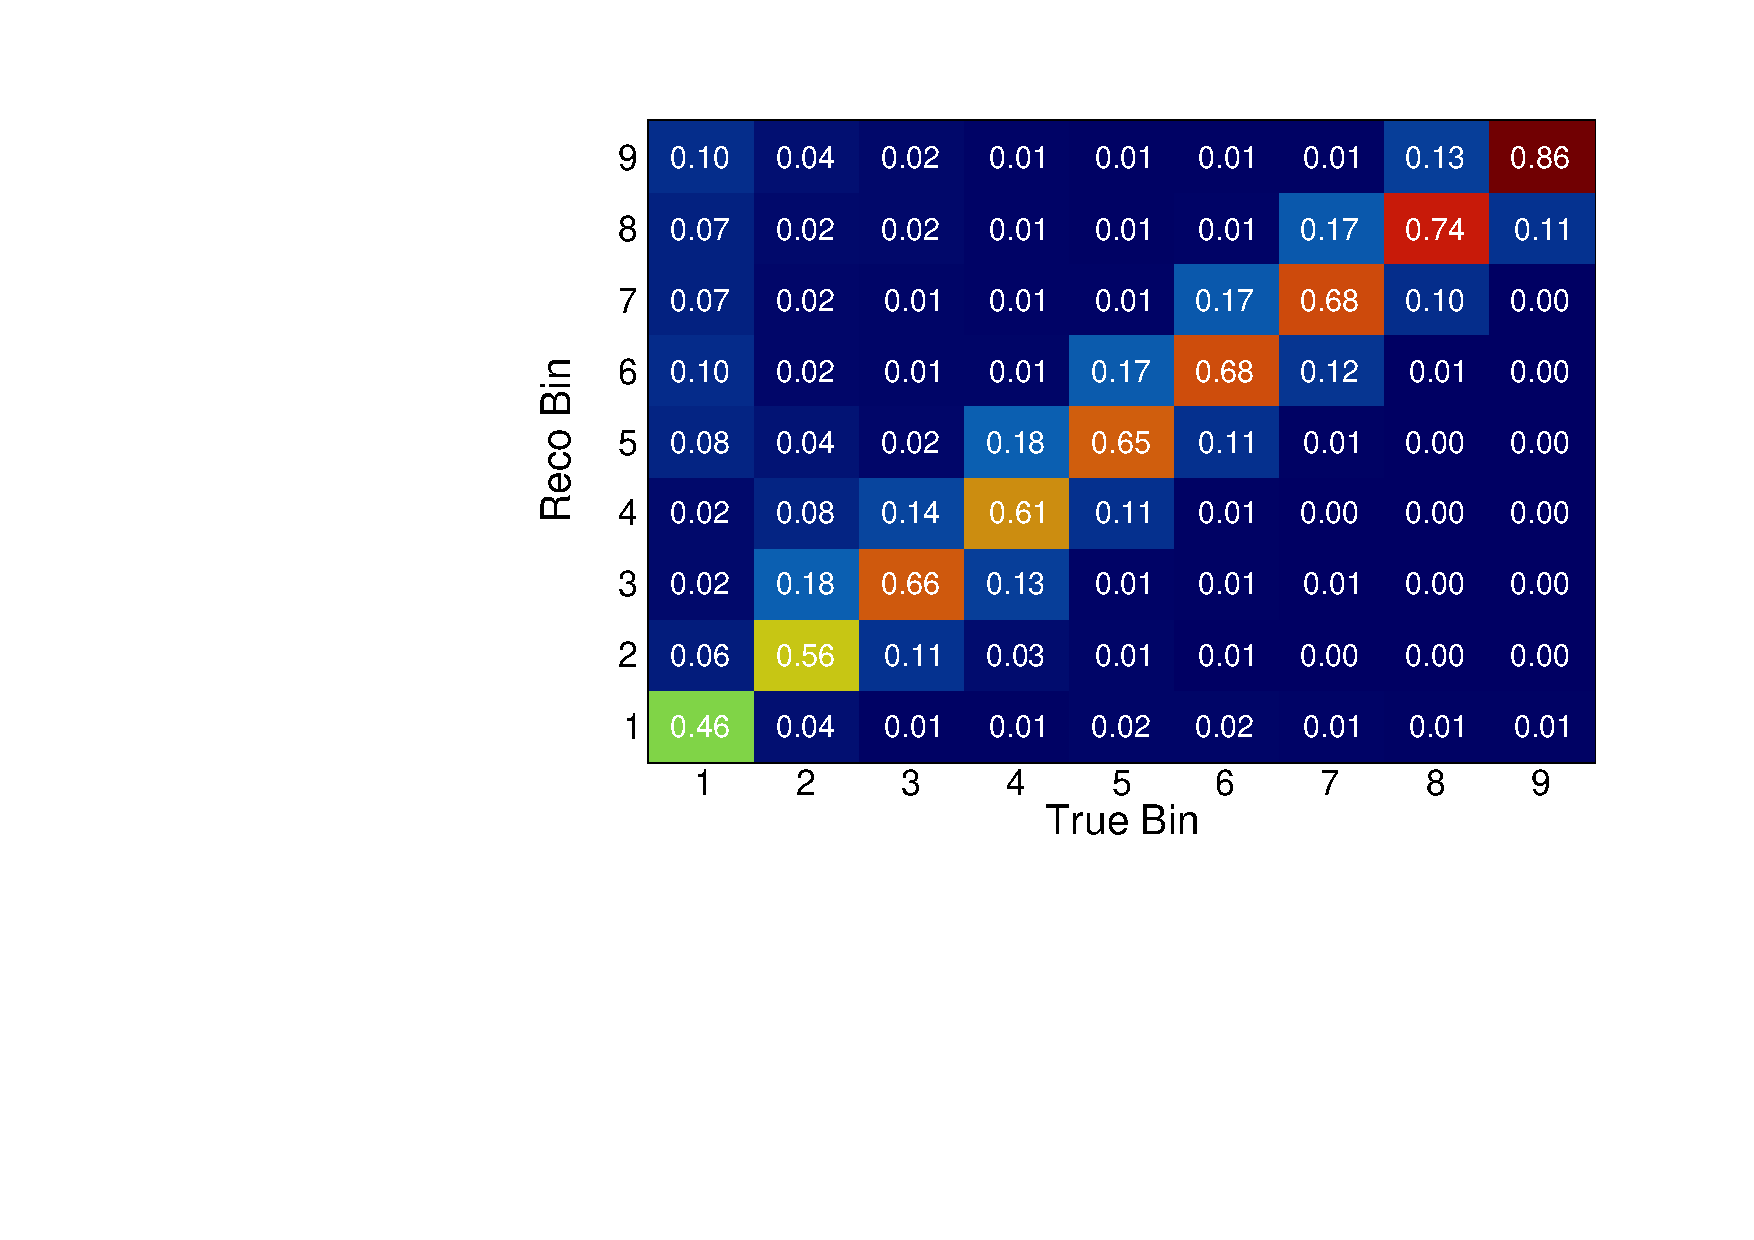
\includegraphics[width=.80\textwidth]{images/XSecCosThetaMu/migration_matrix_2d}
\caption[Smearing Matrix for the $\cos\theta_\mu$ Distributions]{Smearing matrix for the $\cos\theta_\mu$ distributions. It shows the probability that an event in true bin $j$ is observed in reconstructed bin $i$.}
\label{fig:trkangle_migration_matrix_2d}
\end{figure}




Figure~\ref{fig:trkcostheta_all_selected} shows the distributions of the true muon momentum for all generated muons from $\nu_\mu$ \acrshort{cc} interactions in the \acrshort{fv} and for the selected ones. The ratio of these two distributions is shown in Figure~\ref{fig:trkcosthetaefficiecy_mumon_true}, which represents the efficiency as a function of the true muon angle. This corresponds to the efficiency shown in the previous chapter, but here using the final binning. 
%The uncertainties on the efficiency have been calculated in same way as described in Section \ref{sec:migration_pmu}. 

On the right side of Figure~\ref{fig:trkcostheta_eff_smear}, the smeared distributions for both the selected and generated events (\ref{fig:trkcostheta_all_selected_smear}) are shown, and the new efficiency $\tilde{\epsilon}$ as a function of the reconstructed muon angle (\ref{fig:trkcostheta_efficiecy_reco}). This efficiency will be used for the cross-section calculation.

\begin{figure}[t]
\centering
\subfloat[][]
   {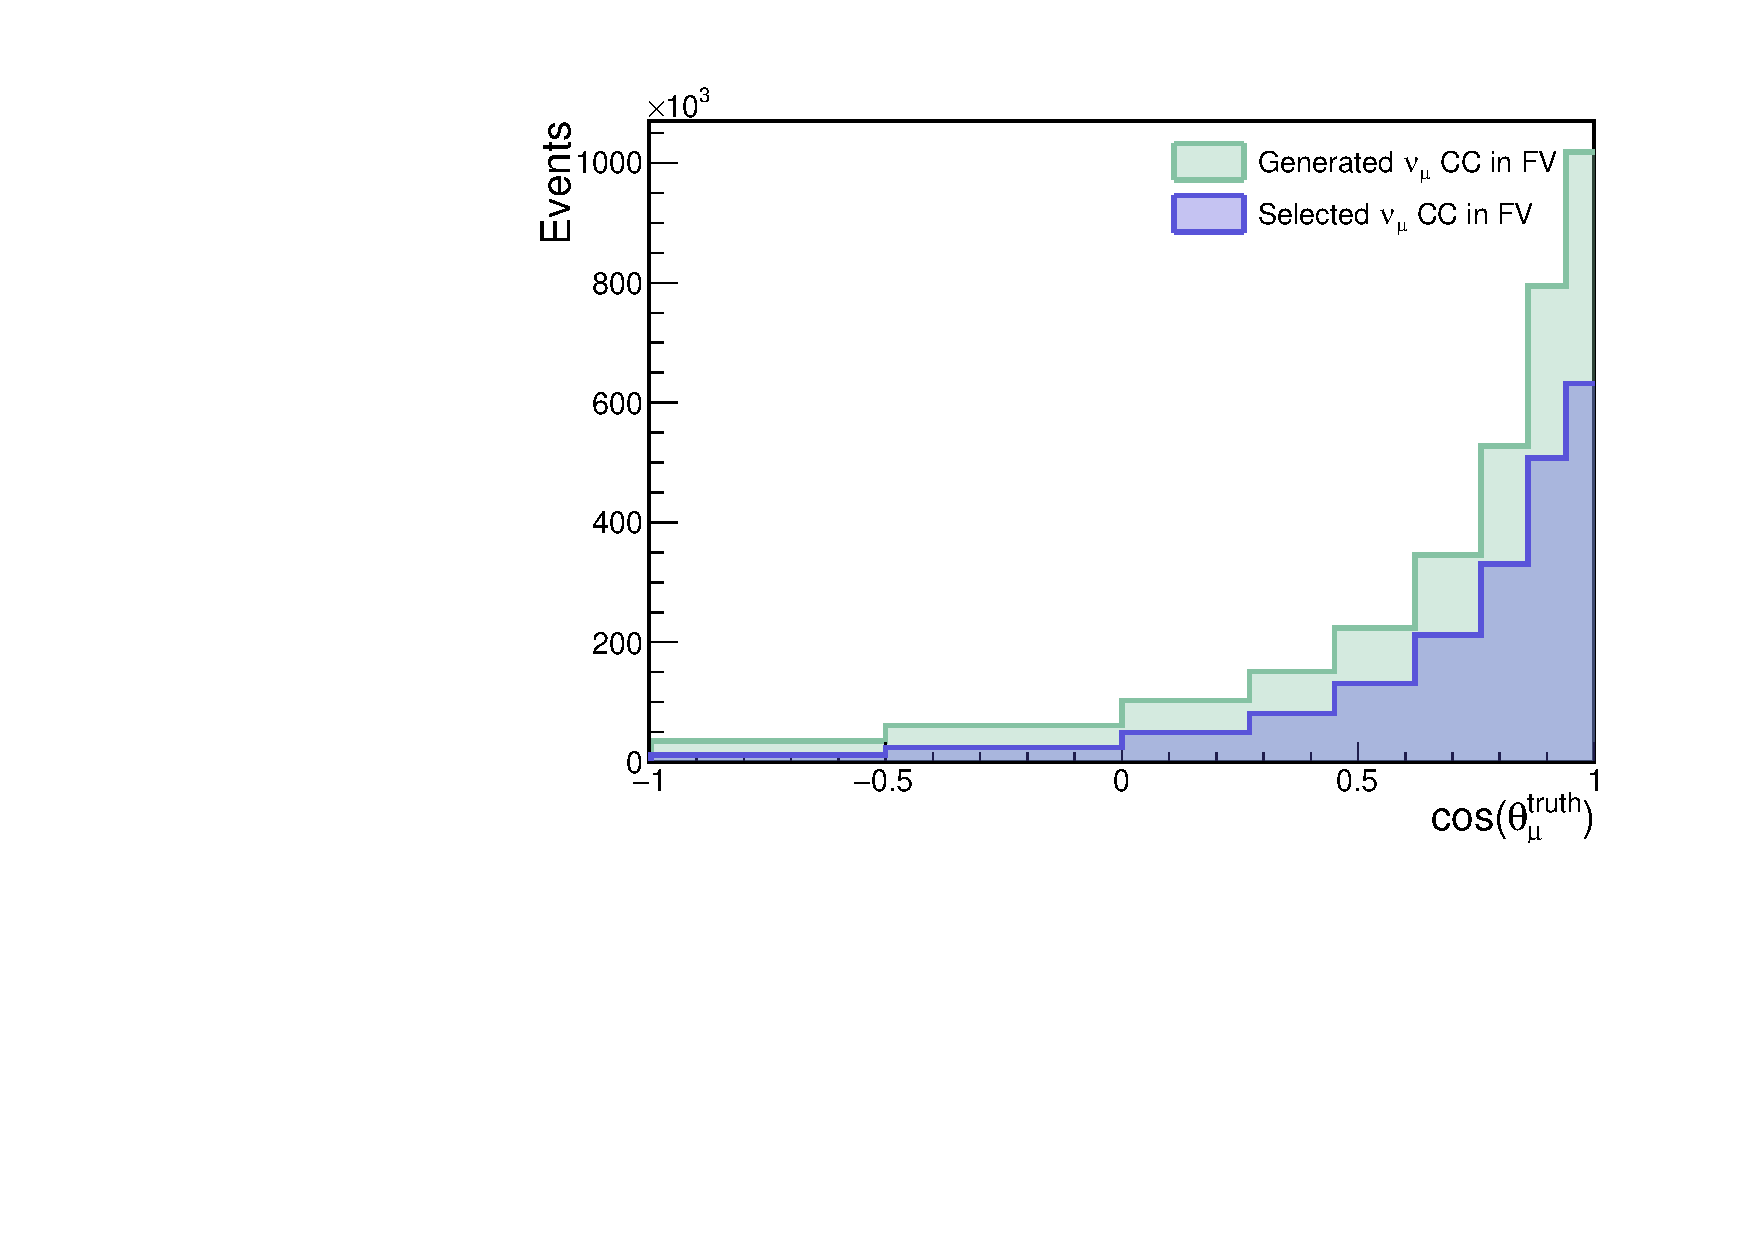
\includegraphics[width=.5\textwidth]{images/XSecCosThetaMu/trkcosthetaall_selected}
   \label{fig:trkcostheta_all_selected}} 
\subfloat[][]
   {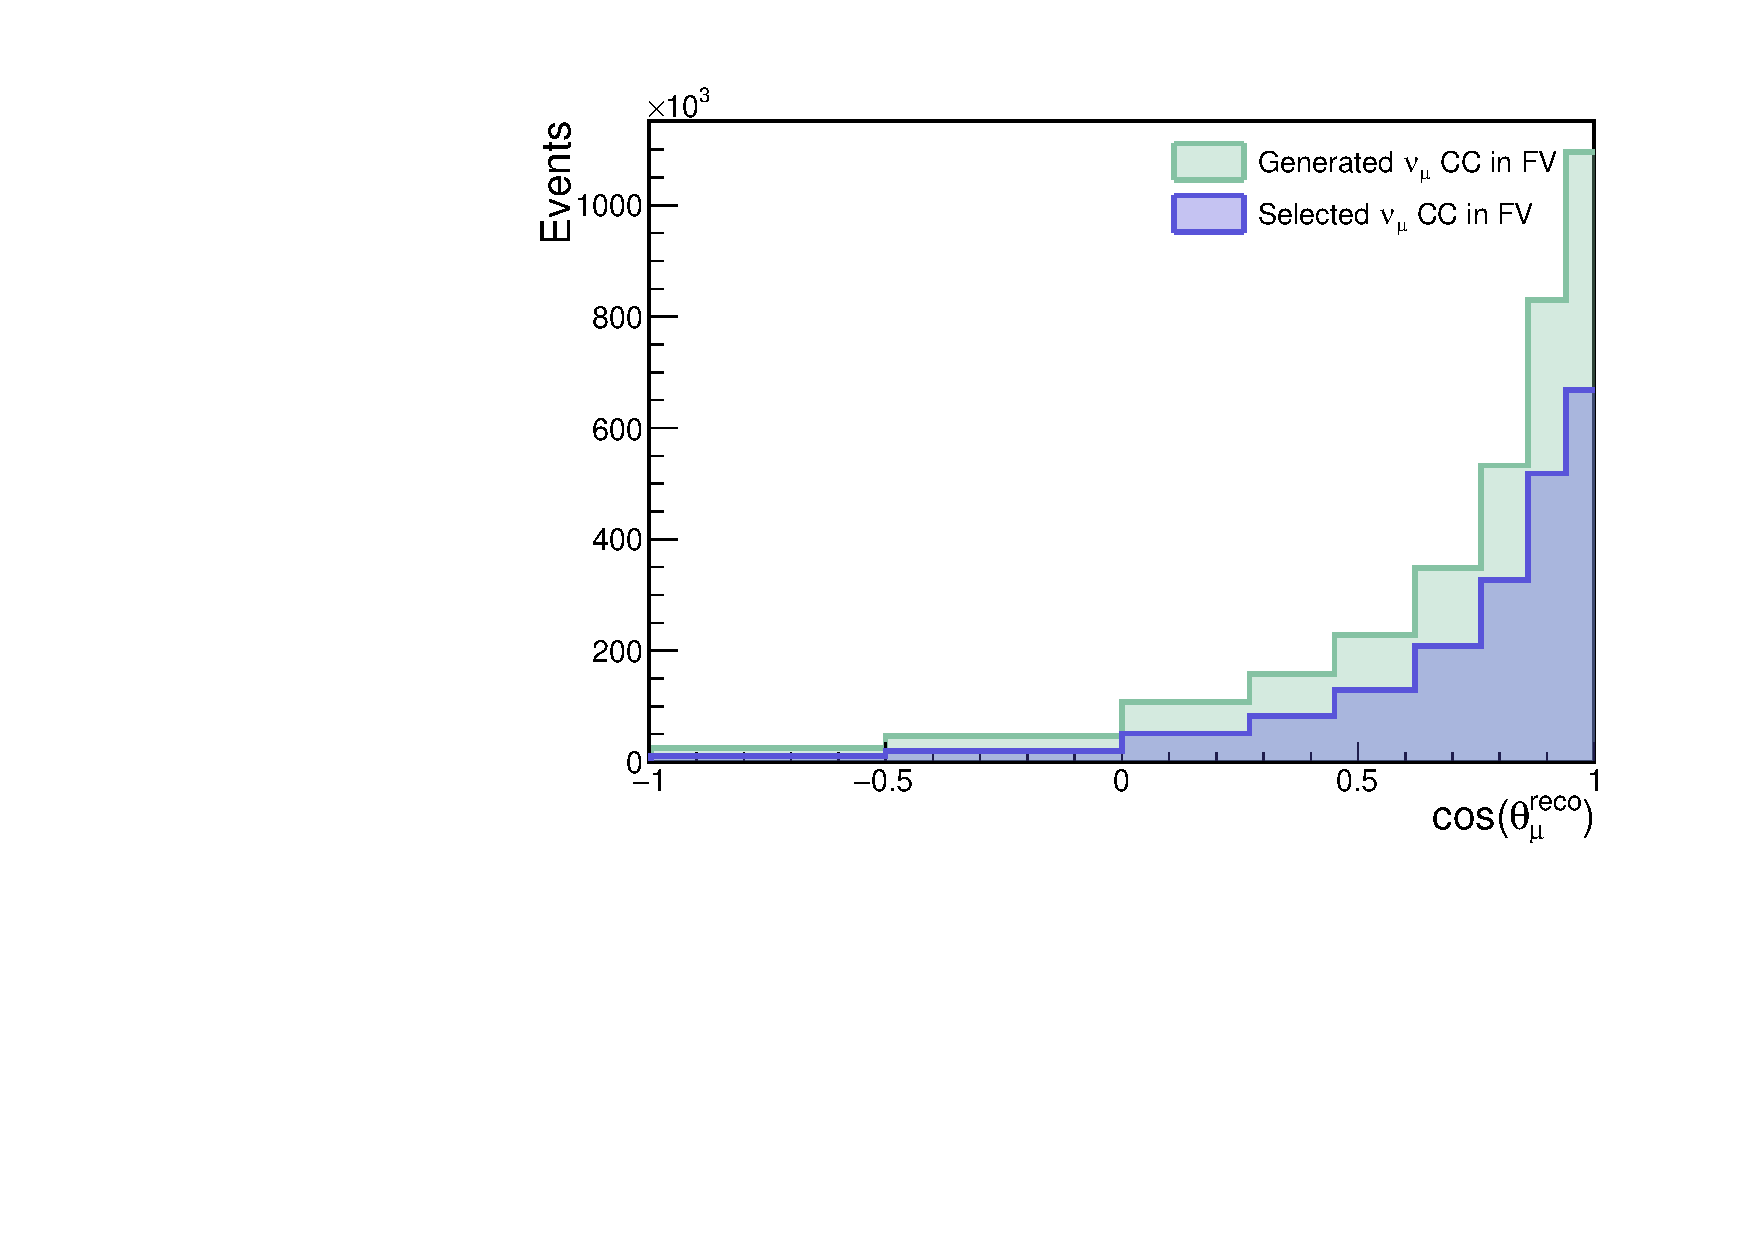
\includegraphics[width=.5\textwidth]{images/XSecCosThetaMu/trkcostheta_all_selected_smear}
   \label{fig:trkcostheta_all_selected_smear}} \\
\subfloat[][]
   {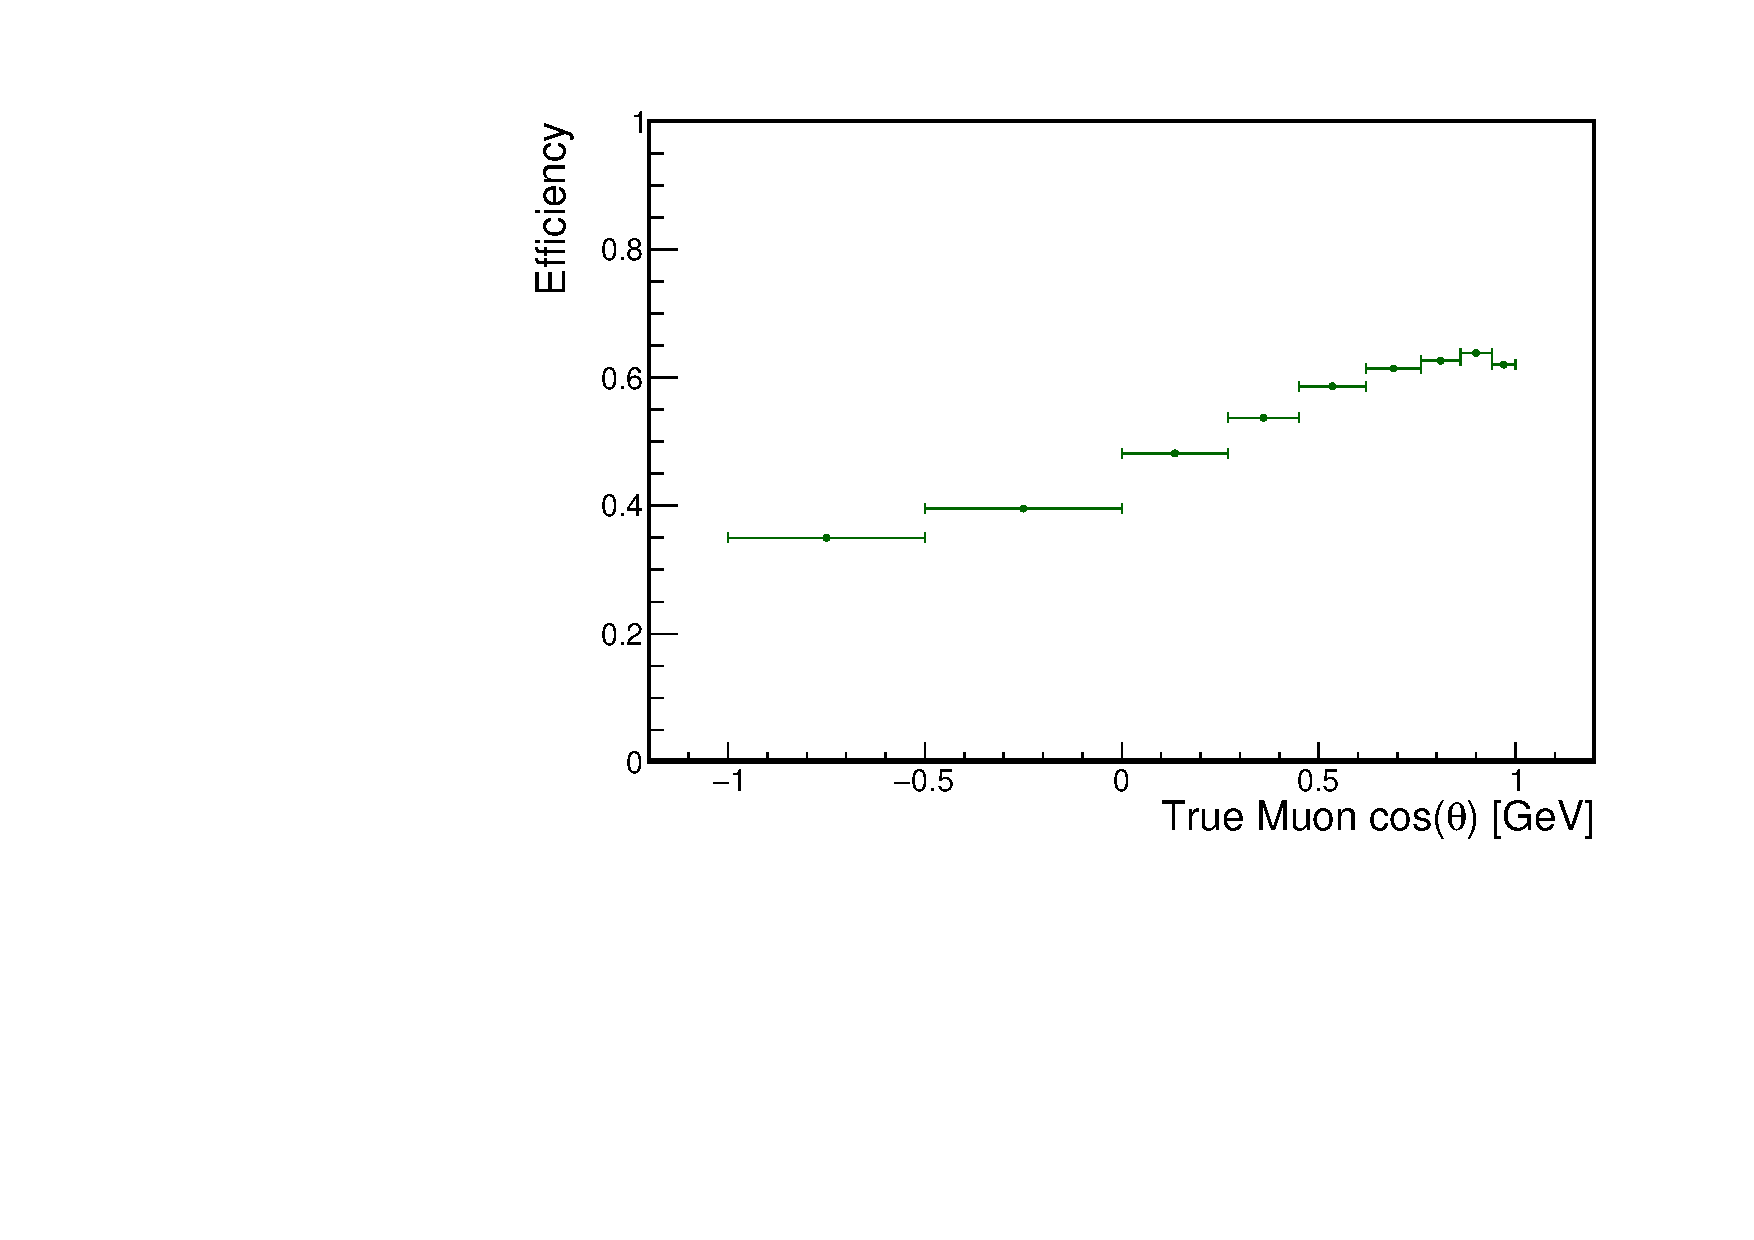
\includegraphics[width=.5\textwidth]{images/XSecCosThetaMu/trkcosthetaefficiecy_mumon_true}
   \label{fig:trkcosthetaefficiecy_mumon_true}} 
\subfloat[][]
   {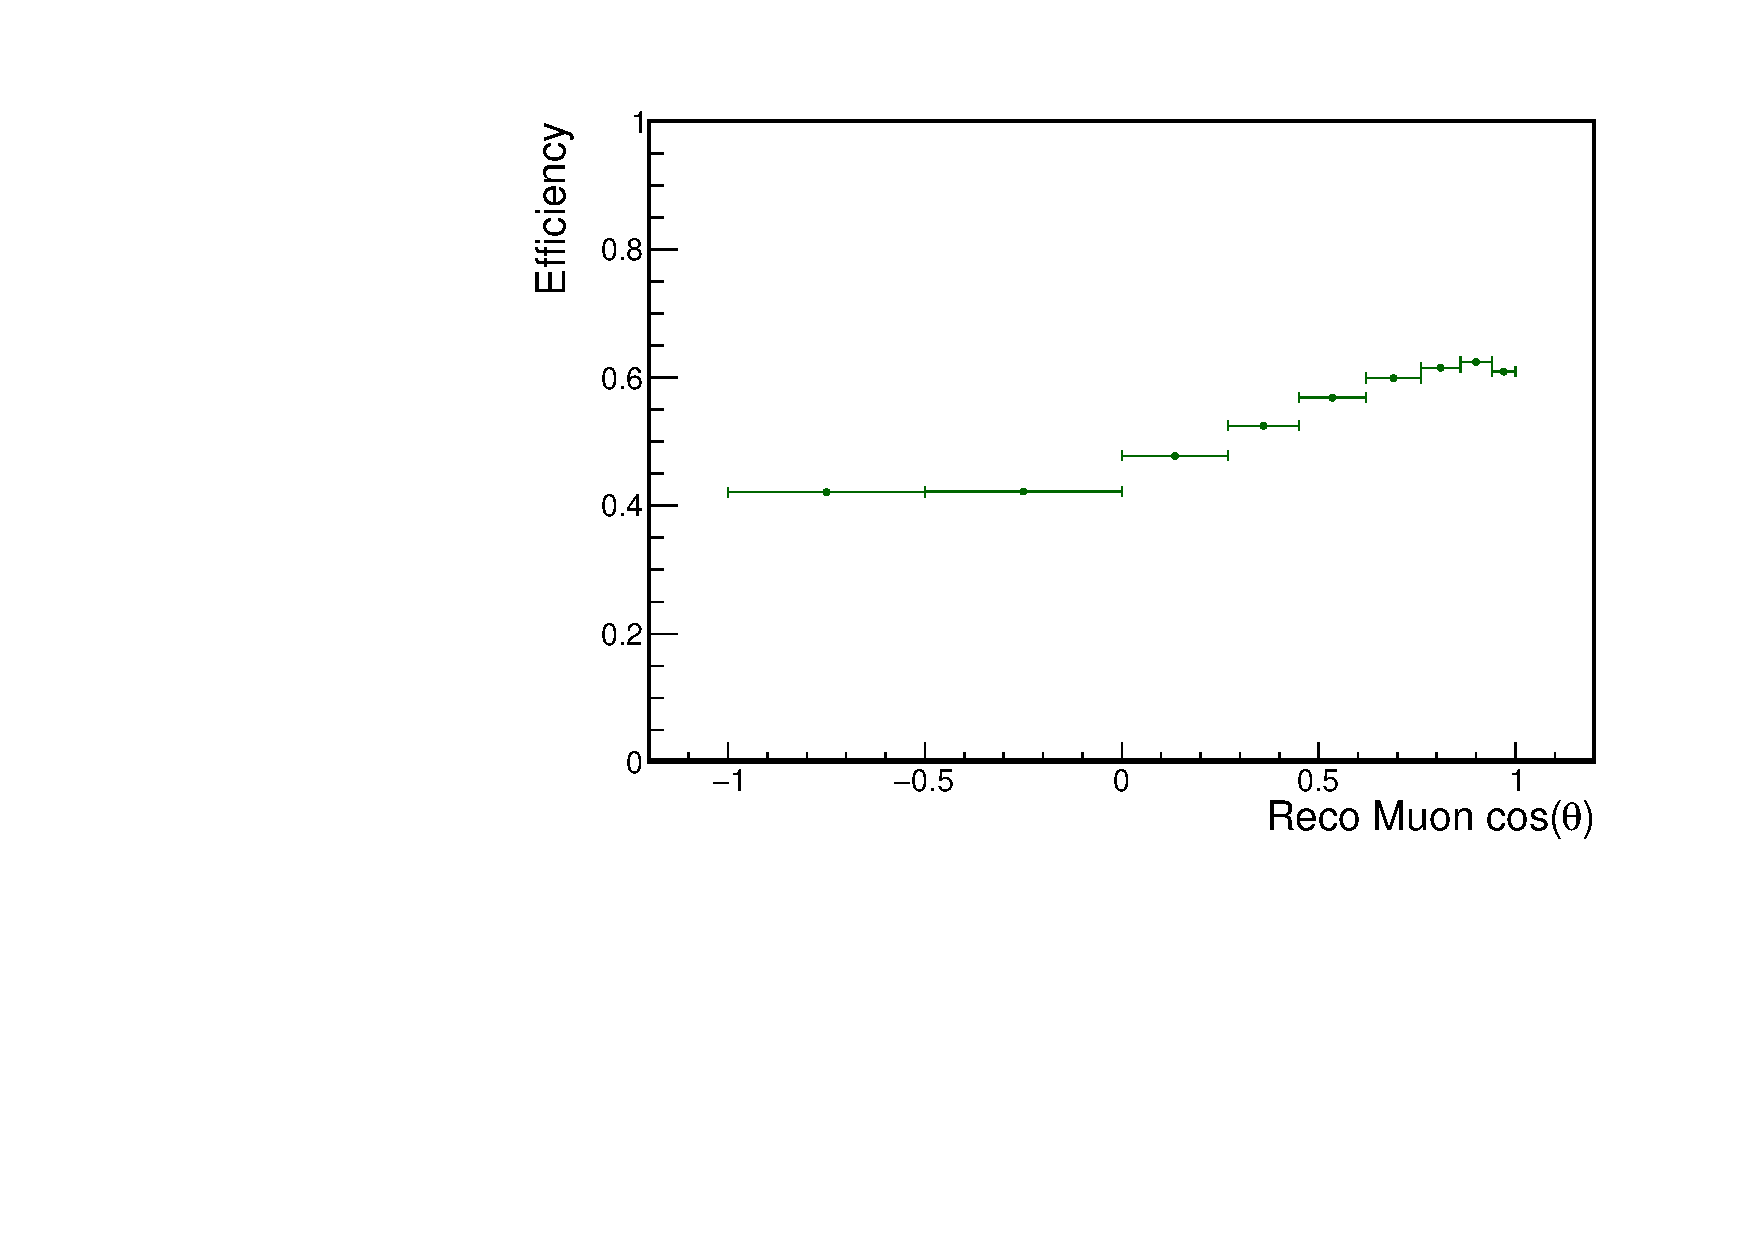
\includegraphics[width=.5\textwidth]{images/XSecCosThetaMu/trkcostheta_efficiecy_reco}
   \label{fig:trkcostheta_efficiecy_reco}} \\
\caption[Simulated $\cos\theta_\mu$ Distributions and Efficiency in $\cos\theta_\mu$ Bins]{Top: distributions of the generated (green) and selected (blue) signal events in terms of the simulated variable $\cos\theta_\mu^\text{truth}$~\protect\subref{fig:trkcostheta_all_selected} and, after smearing, in terms of the reconstructed variable $\cos\theta_\mu^\text{reco}$~\protect\subref{fig:trkcostheta_all_selected_smear}. Bottom: ratio of the distributions above, meaning the efficiency in $\cos\theta_\mu^\text{truth}$~\protect\subref{fig:trkcosthetaefficiecy_mumon_true} and in $\cos\theta_\mu^\text{reco}$~\protect\subref{fig:trkcostheta_efficiecy_reco}.}
\label{fig:trkcostheta_eff_smear}
\end{figure}




%\subsection{Cross Section Central Values}


Putting all the quantities calculated in the previous sections into Equation~\eqref{eq:xsec_differential}, the $\nu_\mu$ \acrshort{cc} inclusive differential cross section on argon in muon angle is extracted and shown in Figure~\ref{fig:trkcostheta_xsec_cv}. 
%The green distributions show the cross section according to the \acrshort{mc} and the light green error bands represent the statistical uncertainty on the \acrshort{mc}. The black data points show the data extracted cross section. The error bars represent the data statistical uncertainty also including the statistical uncertainties on the \acrshort{mc} estimated backgrounds and efficiency. 

\begin{figure}[]
\centering
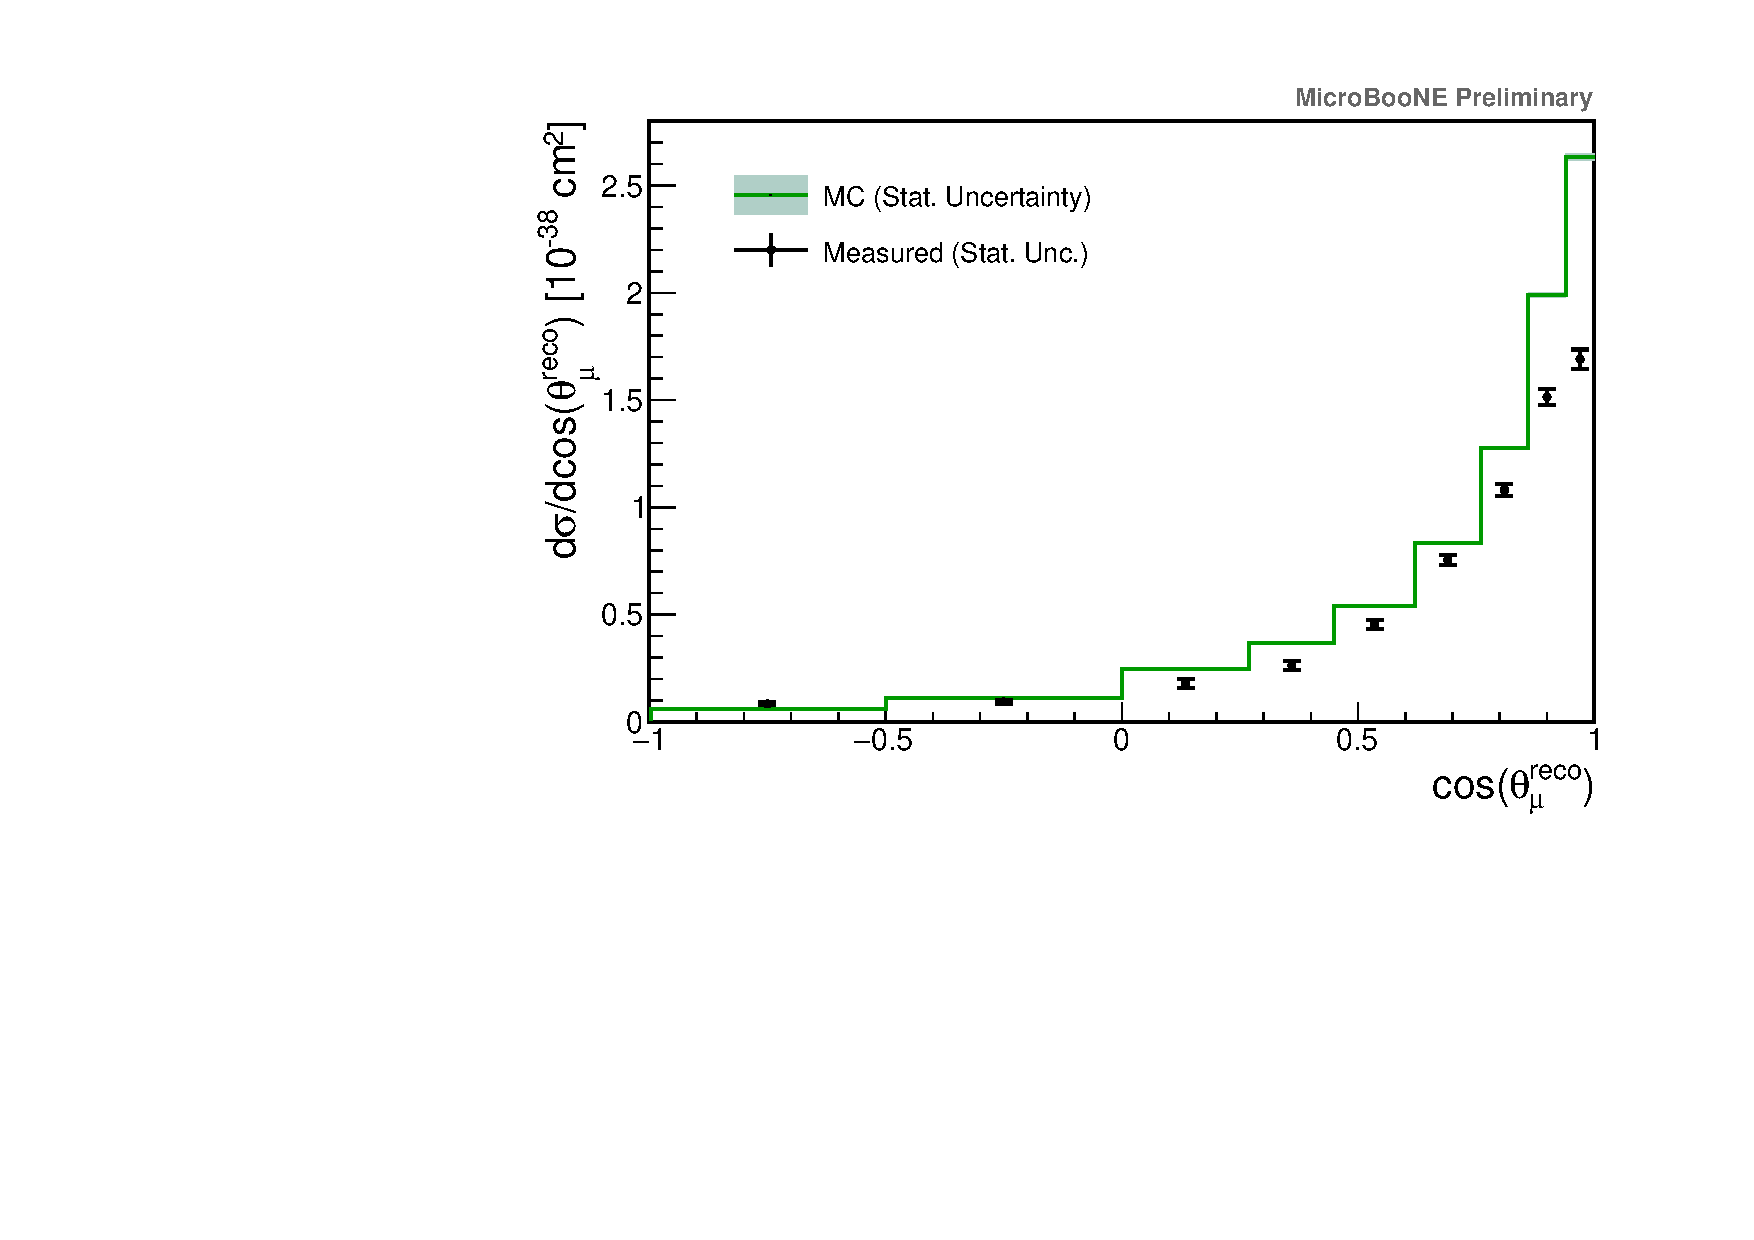
\includegraphics[width=.80\textwidth]{images/XSecCosThetaMu/trkcostheta_xsec}
\caption[$d\sigma/d\cos\theta_\mu$ Single Differential Cross Section (Stat. Unc. Only)]{$\nu_\mu$ \acrshort{cc} inclusive differential cross section on argon per nucleon as a function per nucleonof the cosine of the reconstructed muon polar angle (angle w.r.t. the beam). The black data points show the data extracted cross section, while the green curve shows the \acrshort{mc} predicted cross section. The data error bars and the \acrshort{mc} error bands show the statistical uncertainty only, for data and \acrshort{mc} respectively. Systematic uncertainties are treated in Chapter~\ref{ch:systematics}.}
\label{fig:trkcostheta_xsec_cv}
\end{figure}









\clearpage
%**********************************************************
\section{Double-Differential Cross Section}
\label{sec:mumom_muangle_xsec}

This section shows the calculation of the double-differential cross section in muon momentum $p_\mu$ and cosine of the muon angle $\cos\theta_\mu$. 
The cross section is calculated according to Equation~\eqref{eq:xsec_double_differential} and the number of events per bin is shown in Table~\ref{tab:pmu_costhetamu_events}.


\begin{table}[]
\scriptsize
\begin{adjustwidth}{-2.0cm}{-1.5cm}
\caption[Selected Events Per $(\cos\theta_\mu, p_\mu)$ Bin]{The table shows the number of selected events per $(\cos\theta_\mu, p_\mu)$ reconstructed bin and different categories. Only statistical uncertainties  are shown.}
\label{tab:pmu_costhetamu_events}
\centering
\begin{tabular}{c|cc|ccccccc}
\toprule
    & \multicolumn{2}{c}{Data}    & \multicolumn{6}{c}{\acrshort{mc}} \\
Bin & Selected & Cosmic & $\nu_\mu$ \acrshort{cc} & Cosmic  & \acrshort{outfv} & DIRT & \acrshort{nc} & $\nu_e$ and $\bar{\nu}_e$ & $\bar{\nu}_\mu$ \\
    & Events   & Only   & Signal         & in \acrshort{bnb}  &       &      &    &                           &                 \\
\midrule
1 & 120 $\pm$ 10 & 38.1 $\pm$ 4.3 & 26.5 $\pm$ 1.4 & 9.44 $\pm$ 0.83 & 13.5 $\pm$ 1.0 & 13.64 $\pm$ 0.89 & 12.00 $\pm$ 0.96 & 0.42 $\pm$ 0.15 & 0.36 $\pm$ 0.16 \\ 
2 & 489 $\pm$ 22 & 82.2 $\pm$ 6.3 & 173.3 $\pm$ 3.5 & 15.5 $\pm$ 1.0 & 86.2 $\pm$ 2.5 & 96.3 $\pm$ 2.3 & 24.8 $\pm$ 1.3 & 0.44 $\pm$ 0.17 & 1.46 $\pm$ 0.32 \\ 
3 & 600 $\pm$ 24 & 85.1 $\pm$ 6.4 & 134.6 $\pm$ 3.1 & 12.86 $\pm$ 0.97 & 128.8 $\pm$ 3.1 & 121.9 $\pm$ 2.6 & 14.7 $\pm$ 1.0 & 0.23 $\pm$ 0.11 & 0.75 $\pm$ 0.23 \\ 
4 & 375 $\pm$ 19 & 72.4 $\pm$ 5.9 & 45.52 $\pm$ 1.8 & 11.26 $\pm$ 0.91 & 107.1 $\pm$ 2.8 & 68.3 $\pm$ 1.9 & 2.44 $\pm$ 0.42 & 0.056 $\pm$ 0.056 & 0.31 $\pm$ 0.15 \\ 
5 & 145 $\pm$ 12 & 77.3 $\pm$ 6.1 & 7.95 $\pm$ 0.76 & 25.5 $\pm$ 1.3 & 36.7 $\pm$ 1.6 & 17.5 $\pm$ 1.0 & 0.44 $\pm$ 0.18 & 0 $\pm$ 0.00 & 0.33 $\pm$ 0.17 \\ 
6 & 148 $\pm$ 12 & 75.3 $\pm$ 6.0 & 40.4 $\pm$ 1.7 & 16.2 $\pm$ 1.0 & 14.4 $\pm$ 1.0 & 15.32 $\pm$ 0.94 & 13.7 $\pm$ 1.0 & 0.49 $\pm$ 0.18 & 0.21 $\pm$ 0.12 \\ 
7 & 759 $\pm$ 27 & 372 $\pm$ 13 & 284.4 $\pm$ 4.6 & 56.5 $\pm$ 2.0 & 81.8 $\pm$ 2.4 & 54.2 $\pm$ 1.7 & 22.6 $\pm$ 1.2 & 0.59 $\pm$ 0.18 & 0.74 $\pm$ 0.23 \\ 
8 & 890 $\pm$ 29 & 392 $\pm$ 13 & 283.9 $\pm$ 4.6 & 52.9 $\pm$ 1.9 & 81.1 $\pm$ 2.4 & 42.5 $\pm$ 1.5 & 9.84 $\pm$ 0.85 & 0.28 $\pm$ 0.12 & 0.98 $\pm$ 0.27 \\ 
9 & 496 $\pm$ 22 & 259 $\pm$ 11 & 88.0 $\pm$ 2.5 & 51.7 $\pm$ 1.9 & 31.8 $\pm$ 1.5 & 18.5 $\pm$ 1.0 & 1.80 $\pm$ 0.37 & 0.28 $\pm$ 0.13 & 0.29 $\pm$ 0.14 \\ 
10 & 443 $\pm$ 21 & 317 $\pm$ 12 & 17.4 $\pm$ 1.1 & 91.0 $\pm$ 2.6 & 7.45 $\pm$ 0.74 & 26.7 $\pm$ 1.2 & 3.02 $\pm$ 0.47 & 0.22 $\pm$ 0.11 & 0.14 $\pm$ 0.10 \\ 
11 & 119 $\pm$ 10 & 83.7 $\pm$ 6.4 & 31.2 $\pm$ 1.5 & 15.6 $\pm$ 1.0 & 14.1 $\pm$ 1.0 & 10.02 $\pm$ 0.76 & 10.09 $\pm$ 0.86 & 0.22 $\pm$ 0.11 & 0.22 $\pm$ 0.12 \\ 
12 & 1070 $\pm$ 32 & 600 $\pm$ 17 & 290.8 $\pm$ 4.6 & 87.9 $\pm$ 2.5 & 94.1 $\pm$ 2.6 & 58.7 $\pm$ 1.8 & 23.4 $\pm$ 1.3 & 0.65 $\pm$ 0.20 & 0.96 $\pm$ 0.26 \\ 
13 & 1612 $\pm$ 40 & 886 $\pm$ 20 & 405.9 $\pm$ 5.5 & 123.4 $\pm$ 3.0 & 93.4 $\pm$ 2.6 & 60.9 $\pm$ 1.8 & 11.7 $\pm$ 0.93 & 0.52 $\pm$ 0.17 & 1.62 $\pm$ 0.34 \\ 
14 & 1126 $\pm$ 33 & 708 $\pm$ 18 & 217.8 $\pm$ 4.0 & 144.4 $\pm$ 3.2 & 36.9 $\pm$ 1.6 & 45.6 $\pm$ 1.6 & 4.17 $\pm$ 0.55 & 0.29 $\pm$ 0.14 & 0.59 $\pm$ 0.20 \\ 
15 & 1141 $\pm$ 33 & 869 $\pm$ 20 & 29.27 $\pm$ 1.4 & 262.3 $\pm$ 4.4 & 7.10 $\pm$ 0.72 & 74.9 $\pm$ 2.0 & 3.69 $\pm$ 0.52 & 0.10 $\pm$ 0.10 & 0.0 $\pm$ 0.0 \\ 
16 & 768 $\pm$ 27 & 409 $\pm$ 14 & 265.8 $\pm$ 4.4 & 71.9 $\pm$ 2.3 & 70.8 $\pm$ 2.3 & 38.1 $\pm$ 1.4 & 23.7 $\pm$ 1.3 & 0.77 $\pm$ 0.21 & 2.06 $\pm$ 0.39 \\ 
17 & 978 $\pm$ 31 & 446 $\pm$ 14 & 413 $\pm$ 5.5 & 67.6 $\pm$ 2.2 & 65.8 $\pm$ 2.2 & 30.8 $\pm$ 1.3 & 8.99 $\pm$ 0.81 & 0.29 $\pm$ 0.12 & 2.15 $\pm$ 0.40 \\ 
18 & 840 $\pm$ 28 & 351 $\pm$ 13 & 339.4 $\pm$ 5.0 & 79.7 $\pm$ 2.4 & 31.8 $\pm$ 1.5 & 19.7 $\pm$ 1.0 & 3.99 $\pm$ 0.54 & 0.063 $\pm$ 0.063 & 1.82 $\pm$ 0.38 \\ 
19 & 673 $\pm$ 25 & 502 $\pm$ 15 & 51.6 $\pm$ 1.9 & 184.6 $\pm$ 3.7 & 8.16 $\pm$ 0.77 & 41.5 $\pm$ 1.5 & 2.45 $\pm$ 0.42 & 0.147 $\pm$ 0.087 & 0.15 $\pm$ 0.10 \\ 
20 & 597 $\pm$ 24 & 255 $\pm$ 11 & 270.4 $\pm$ 4.4 & 48.5 $\pm$ 1.9 & 60.5 $\pm$ 2.1 & 28.0 $\pm$ 1.2 & 29.9 $\pm$ 1.4 & 0.69 $\pm$ 0.19 & 1.93 $\pm$ 0.37 \\ 
21 & 896 $\pm$ 29 & 283 $\pm$ 11 & 513.2 $\pm$ 6.1 & 44.1 $\pm$ 1.8 & 71.3 $\pm$ 2.3 & 20.2 $\pm$ 1.0 & 13.01 $\pm$ 0.98 & 0.49 $\pm$ 0.17 & 3.13 $\pm$ 0.48 \\ 
22 & 1029 $\pm$ 32 & 253 $\pm$ 11 & 656.8 $\pm$ 6.9 & 52.9 $\pm$ 1.9 & 55.9 $\pm$ 2.0 & 14.03 $\pm$ 0.90 & 4.58 $\pm$ 0.57 & 0.073 $\pm$ 0.073 & 2.18 $\pm$ 0.40 \\ 
23 & 649 $\pm$ 25 & 372 $\pm$ 13 & 161.1 $\pm$ 3.4 & 141.3 $\pm$ 3.2 & 14.6 $\pm$ 1.0 & 22.8 $\pm$ 1.1 & 2.50 $\pm$ 0.42 & 0.30 $\pm$ 0.14 & 0.71 $\pm$ 0.22 \\ 
24 & 382 $\pm$ 19 & 106.7 $\pm$ 7.2 & 233.5 $\pm$ 4.1 & 26.0 $\pm$ 1.3 & 48.6 $\pm$ 1.9 & 18.6 $\pm$ 1.0 & 30.2 $\pm$ 1.4 & 0.66 $\pm$ 0.19 & 1.79 $\pm$ 0.36 \\ 
25 & 741 $\pm$ 27 & 139.5 $\pm$ 8.2 & 510.5 $\pm$ 6.1 & 21.3 $\pm$ 1.2 & 63.0 $\pm$ 2.1 & 15.76 $\pm$ 0.95 & 13.7 $\pm$ 1.0 & 0.36 $\pm$ 0.15 & 3.52 $\pm$ 0.51 \\ 
26 & 1241 $\pm$ 35 & 132.6 $\pm$ 8.0 & 988.2 $\pm$ 8.5 & 26.7 $\pm$ 1.4 & 84.3 $\pm$ 2.5 & 12.00 $\pm$ 0.83 & 9.19 $\pm$ 0.82 & 0.47 $\pm$ 0.18 & 6.20 $\pm$ 0.70 \\ 
27 & 648 $\pm$ 25 & 186 $\pm$ 9.5 & 415.4 $\pm$ 5.5 & 79.1 $\pm$ 2.4 & 33.0 $\pm$ 1.5 & 10.83 $\pm$ 0.79 & 3.30 $\pm$ 0.49 & 0.137 $\pm$ 0.097 & 2.87 $\pm$ 0.46 \\ 
28 & 211 $\pm$ 14 & 54.8 $\pm$ 5.1 & 156.5 $\pm$ 3.4 & 10.19 $\pm$ 0.87 & 31.4 $\pm$ 1.5 & 8.65 $\pm$ 0.70 & 26.3 $\pm$ 1.4 & 0.85 $\pm$ 0.22 & 1.77 $\pm$ 0.36 \\ 
29 & 398 $\pm$ 19 & 50.4 $\pm$ 4.9 & 383.9 $\pm$ 5.3 & 8.92 $\pm$ 0.81 & 50.8 $\pm$ 1.9 & 13.60 $\pm$ 0.88 & 15.1 $\pm$ 1.0 & 0.77 $\pm$ 0.21 & 3.14 $\pm$ 0.48 \\ 
30 & 1141 $\pm$ 33 & 53.8 $\pm$ 5.1 & 1037.0 $\pm$ 8.7 & 10.62 $\pm$ 0.88 & 90.2 $\pm$ 2.5 & 12.93 $\pm$ 0.86 & 10.13 $\pm$ 0.86 & 0.17 $\pm$ 0.10 & 7.04 $\pm$ 0.73 \\ 
31 & 791 $\pm$ 28 & 38.1 $\pm$ 4.3 & 718.3 $\pm$ 7.3 & 12.64 $\pm$ 0.97 & 54.3 $\pm$ 2.0 & 2.96 $\pm$ 0.41 & 4.04 $\pm$ 0.54 & 0.21 $\pm$ 0.12 & 5.91 $\pm$ 0.68 \\ 
32 & 146 $\pm$ 12 & 41.6 $\pm$ 4.5 & 114.8 $\pm$ 2.9 & 15.2 $\pm$ 1.0 & 9.07 $\pm$ 0.81 & 2.03 $\pm$ 0.34 & 0.89 $\pm$ 0.25 & 0.0 $\pm$ 0.0 & 1.10 $\pm$ 0.32 \\ 
33 & 170 $\pm$ 13 & 33.7 $\pm$ 4.0 & 118.0 $\pm$ 2.9 & 5.85 $\pm$ 0.65 & 23.3 $\pm$ 1.3 & 8.27 $\pm$ 0.69 & 21.8 $\pm$ 1.2 & 0.65 $\pm$ 0.21 & 1.46 $\pm$ 0.33 \\ 
34 & 312 $\pm$ 17 & 12.7 $\pm$ 2.4 & 315.2 $\pm$ 4.8 & 4.01 $\pm$ 0.54 & 45.9 $\pm$ 1.8 & 18.8 $\pm$ 1.0 & 18.1 $\pm$ 1.1 & 0.59 $\pm$ 0.19 & 2.52 $\pm$ 0.43 \\ 
35 & 1080 $\pm$ 32 & 12.7 $\pm$ 2.4 & 1046.0 $\pm$ 8.8 & 3.27 $\pm$ 0.49 & 102.6 $\pm$ 2.7 & 22.5 $\pm$ 1.1 & 11.81 $\pm$ 0.93 & 0.79 $\pm$ 0.23 & 10.05 $\pm$ 0.88 \\ 
36 & 1079 $\pm$ 32 & 15.6 $\pm$ 2.7 & 1207.0 $\pm$ 9.4 & 3.05 $\pm$ 0.47 & 99.1 $\pm$ 2.7 & 6.42 $\pm$ 0.61 & 5.89 $\pm$ 0.65 & 0.28 $\pm$ 0.14 & 13.01 $\pm$ 0.99 \\ 
37 & 234 $\pm$ 15 & 14.1 $\pm$ 2.6 & 359.9 $\pm$ 5.1 & 4.53 $\pm$ 0.58 & 29.8 $\pm$ 1.4 & 0.98 $\pm$ 0.23 & 1.95 $\pm$ 0.37 & 0.21 $\pm$ 0.12 & 4.86 $\pm$ 0.61 \\ 
38 & 108 $\pm$ 10 & 11.2 $\pm$ 2.3 & 96.9 $\pm$ 2.6 & 2.85 $\pm$ 0.45 & 18.9 $\pm$ 1.1 & 8.59 $\pm$ 0.70 & 22.4 $\pm$ 1.2 & 0.91 $\pm$ 0.23 & 0.95 $\pm$ 0.26 \\ 
39 & 243 $\pm$ 15 & 5.3 $\pm$ 1.6 & 232.5 $\pm$ 4.1 & 0.74 $\pm$ 0.23 & 36.4 $\pm$ 1.6 & 22.7 $\pm$ 1.1 & 20.7 $\pm$ 1.2 & 0.91 $\pm$ 0.23 & 3.29 $\pm$ 0.49 \\ 
40 & 798 $\pm$ 28 & 7.8 $\pm$ 1.9 & 821.2 $\pm$ 7.8 & 0.70 $\pm$ 0.22 & 92.4 $\pm$ 2.6 & 36.2 $\pm$ 1.4 & 13.17 $\pm$ 0.97 & 0.61 $\pm$ 0.20 & 10.81 $\pm$ 0.90 \\ 
41 & 977 $\pm$ 31 & 2.4 $\pm$ 1.0 & 1223.0 $\pm$ 9.5 & 0.51 $\pm$ 0.19 & 114.6 $\pm$ 2.9 & 24.5 $\pm$ 1.1 & 5.88 $\pm$ 0.73 & 0.073 $\pm$ 0.073 & 20.1 $\pm$ 1.2 \\ 
42 & 330 $\pm$ 18 & 3.4 $\pm$ 1.2 & 553.5 $\pm$ 6.3 & 0.50 $\pm$ 0.19 & 52.2 $\pm$ 1.9 & 12.54 $\pm$ 0.84 & 2.37 $\pm$ 0.41 & 0.088 $\pm$ 0.088 & 9.81 $\pm$ 0.97 \\ 
\bottomrule
\end{tabular}
\end{adjustwidth}
\end{table}



%\subsection{Migration Matrix for the Double-Differential Cross Section}

As done for the single differential cross sections, the true distributions need to be smeared in order to calculate the efficiency as a function of reconstructed muon momentum and muon angle, using Equation~\eqref{eq:eff_smear}. The migration matrix is calculated according to this formula and is illustrated in Figure~\ref{fig:full_migration_matrix_4d}.
The \g simulator does not simulate events in the region of phase space covered by true bin 5 and 10. By looking at Figure~\ref{fig:polybins}, this is a region of phase space where the muon is emitted in the opposite direction compared to the neutrino one, and has high momentum. The simulator does not produce such events as they would violate the conservation of momentum. For this reason, the value of the matrix for those specific bins is set to $S_{5, 5} = S_{10,10} = 1$ and $S_{i,5} = 0 \, \forall i \neq 5$ and $S_{i,10} = 0 \, \forall i \neq 10$.

\begin{figure}[]
\centering
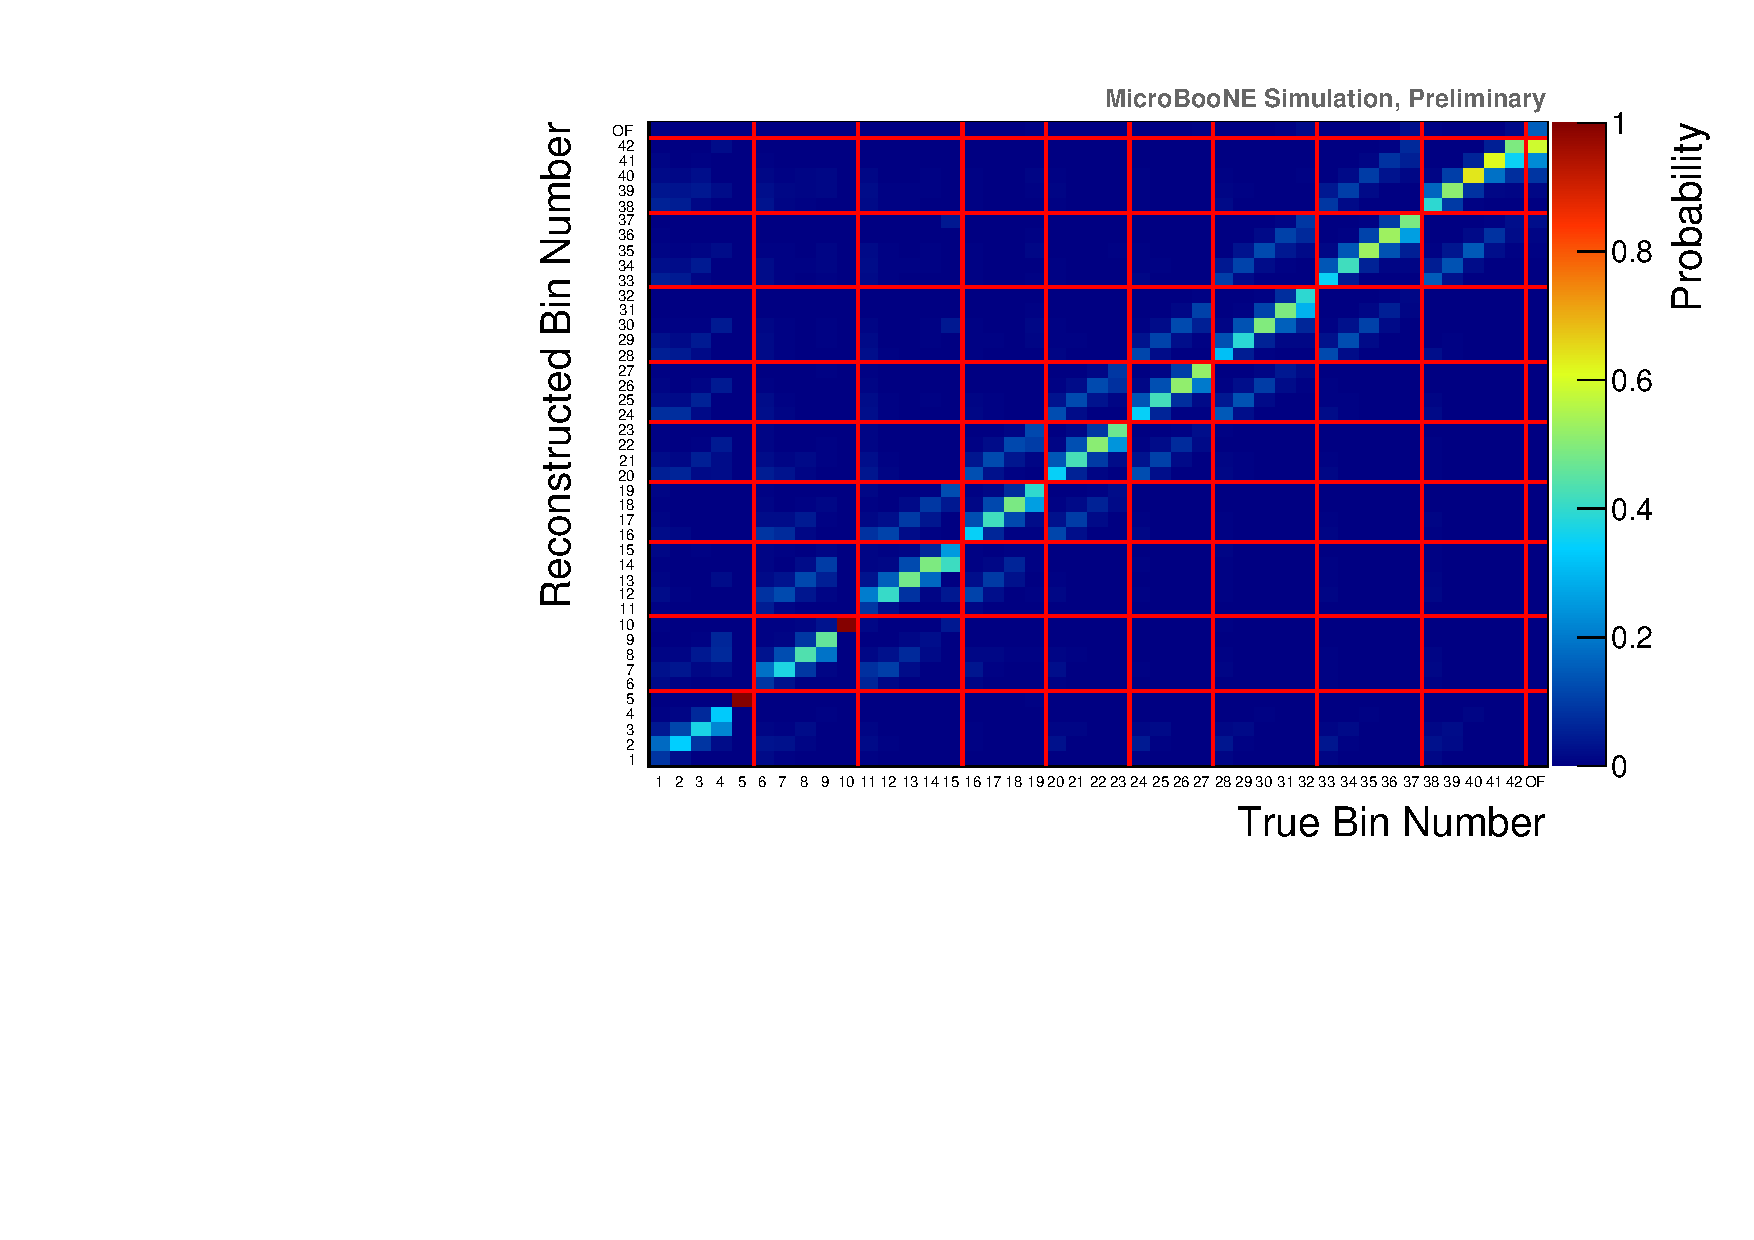
\includegraphics[width=1.0\textwidth]{images/XSecPmuCosThetaMu/full_migration_matrix_4d_poly}
\caption[Migration Matrix for the Double-Differential Cross Section]{Migration matrix for the double-differential cross section in $p_\mu$ and $\cos\theta_\mu$. It shows the probability that an event in a certain true bin ($y$ axis) is observed in a reconstructed bin ($x$ axis).}
\label{fig:full_migration_matrix_4d}
\end{figure}

Figure~\ref{fig:trkcostheta_trkmumom_all} shows the distributions of the true muon momentum for all generated muons from $\nu_\mu$ \acrshort{cc} interactions in the \acrshort{fv} and Figure~\ref{fig:trkcostheta_trkmumom_selected}  shows the same distribution only for the selected events. The ratio of these two distributions is shown in Figure~\ref{fig:trkcostheta_trkmumom_efficiecy_true}, which shows the efficiency as a function of the true muon momentum. 
%The uncertainties on the efficiency have been calculated in same way as described in Section \ref{sec:migration_pmu}. 

On the right side of Figure~\ref{fig:trkcostheta_trkmom_eff_smear}, the smeared distributions for both the selected and generated events (\ref{fig:trkcostheta_trkmumom_all_smear}, \ref{fig:trkcostheta_trkmumom_selected_smear}), and the new efficiency $\tilde{\epsilon}$ as a function of the reconstructed muon momentum (\ref{fig:trkcostheta_trkmumom__efficiecy_reco}) are shown. This 2-dimensional efficiency will be used for the cross-section calculation.

\begin{figure}[]
\centering
\subfloat[][Before smearing.]
   {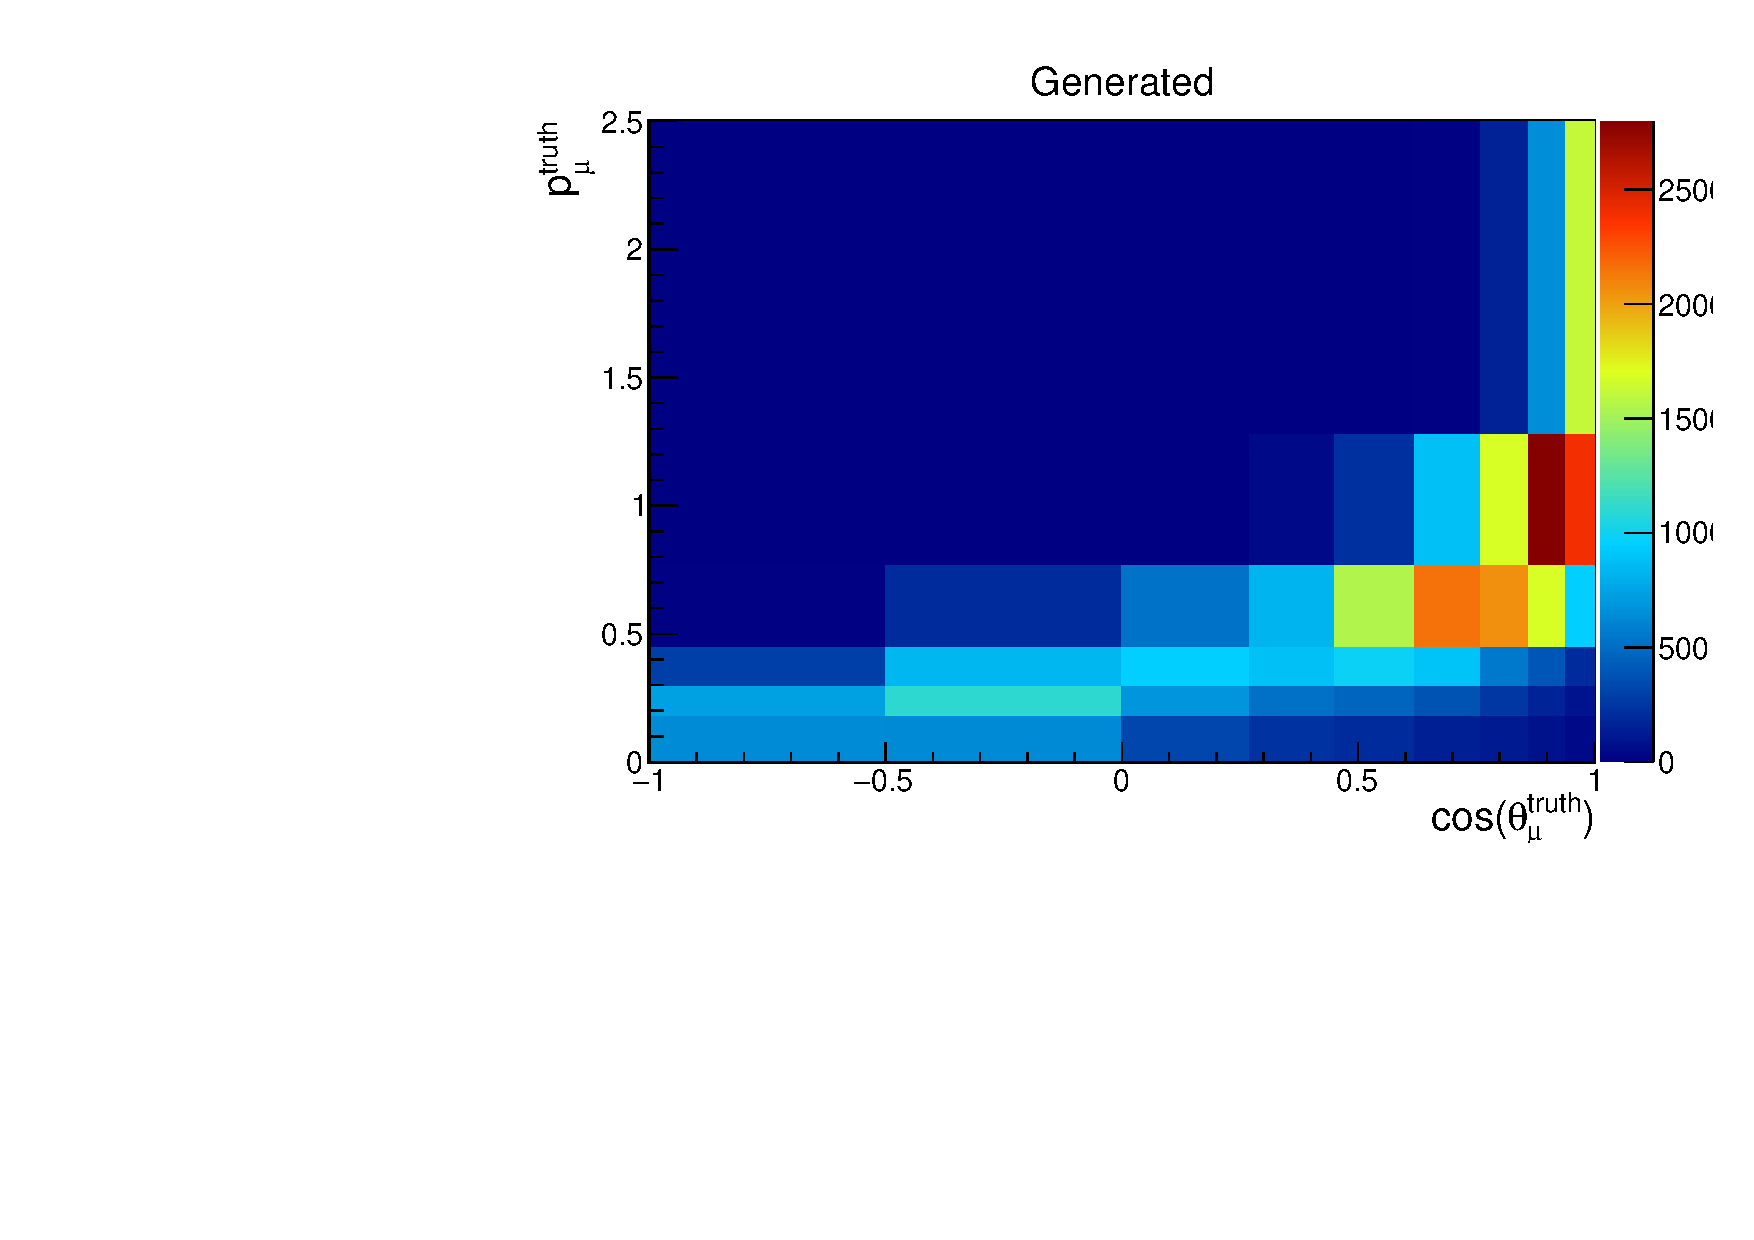
\includegraphics[width=.45\textwidth]{images/XSecPmuCosThetaMu/trkcostheta_trkmumom_all_truth}
   \label{fig:trkcostheta_trkmumom_all}} \quad
\subfloat[][After smearing.]
   {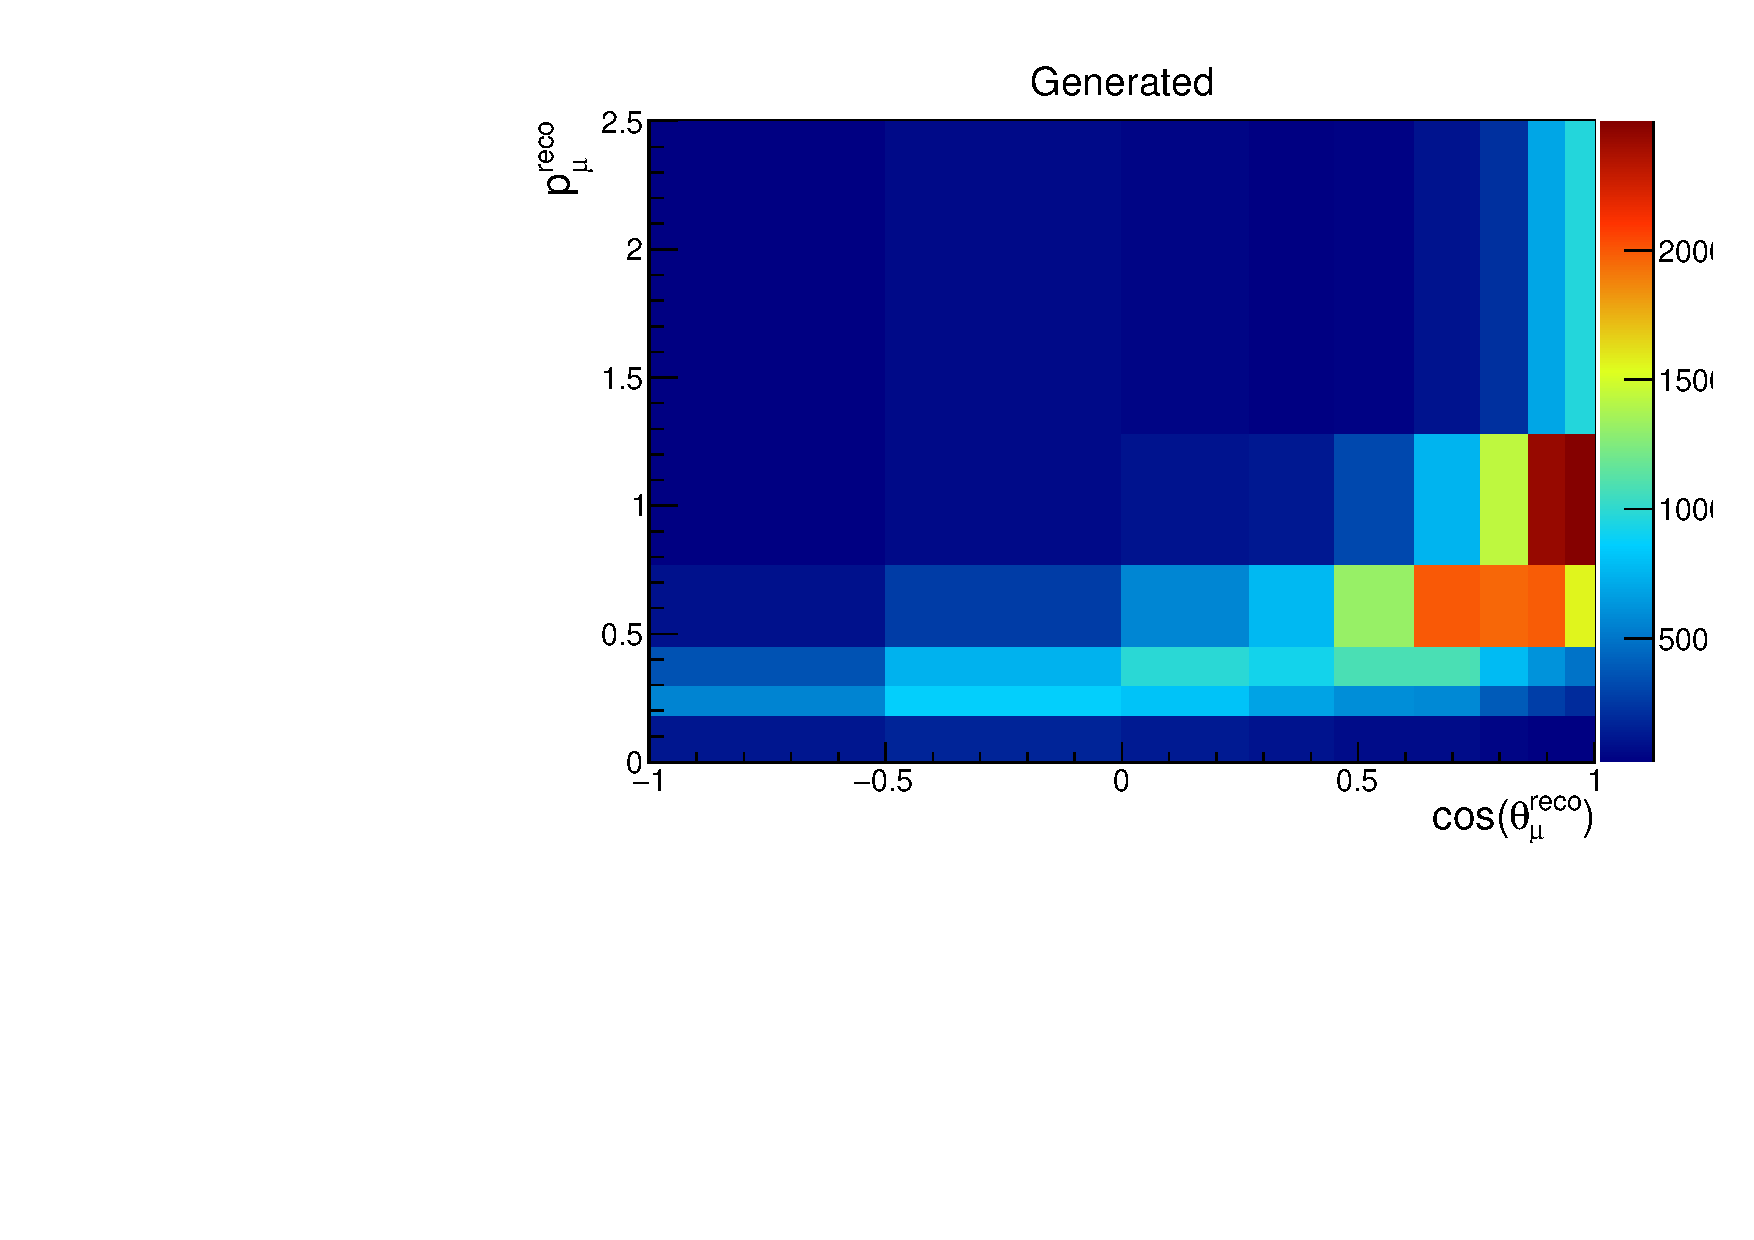
\includegraphics[width=.45\textwidth]{images/XSecPmuCosThetaMu/trkcostheta_trkmumom_all_smeared}
   \label{fig:trkcostheta_trkmumom_all_smear}} \quad
\subfloat[][Before smearing.]
   {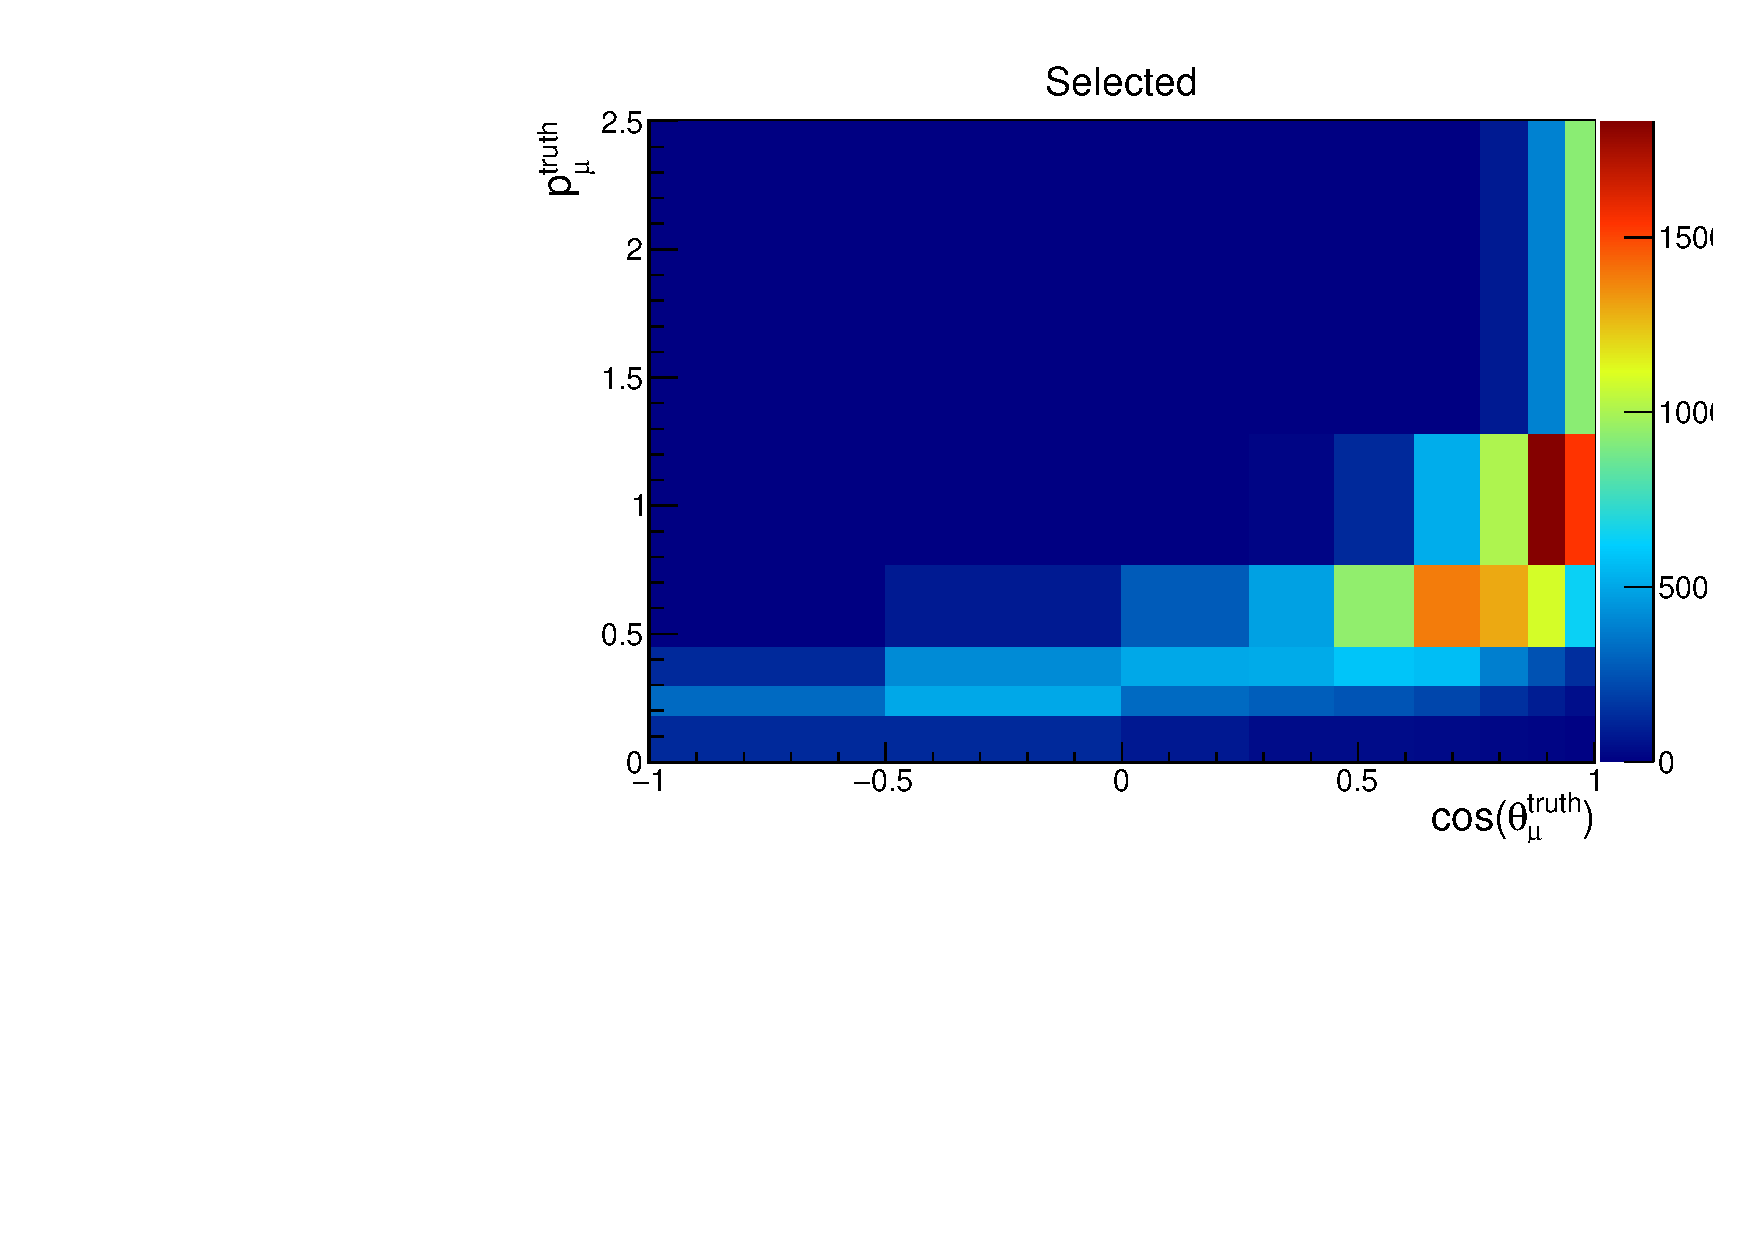
\includegraphics[width=.45\textwidth]{images/XSecPmuCosThetaMu/trkcostheta_trkmumom_selected_truth}
   \label{fig:trkcostheta_trkmumom_selected}} \quad
\subfloat[][After smearing.]
   {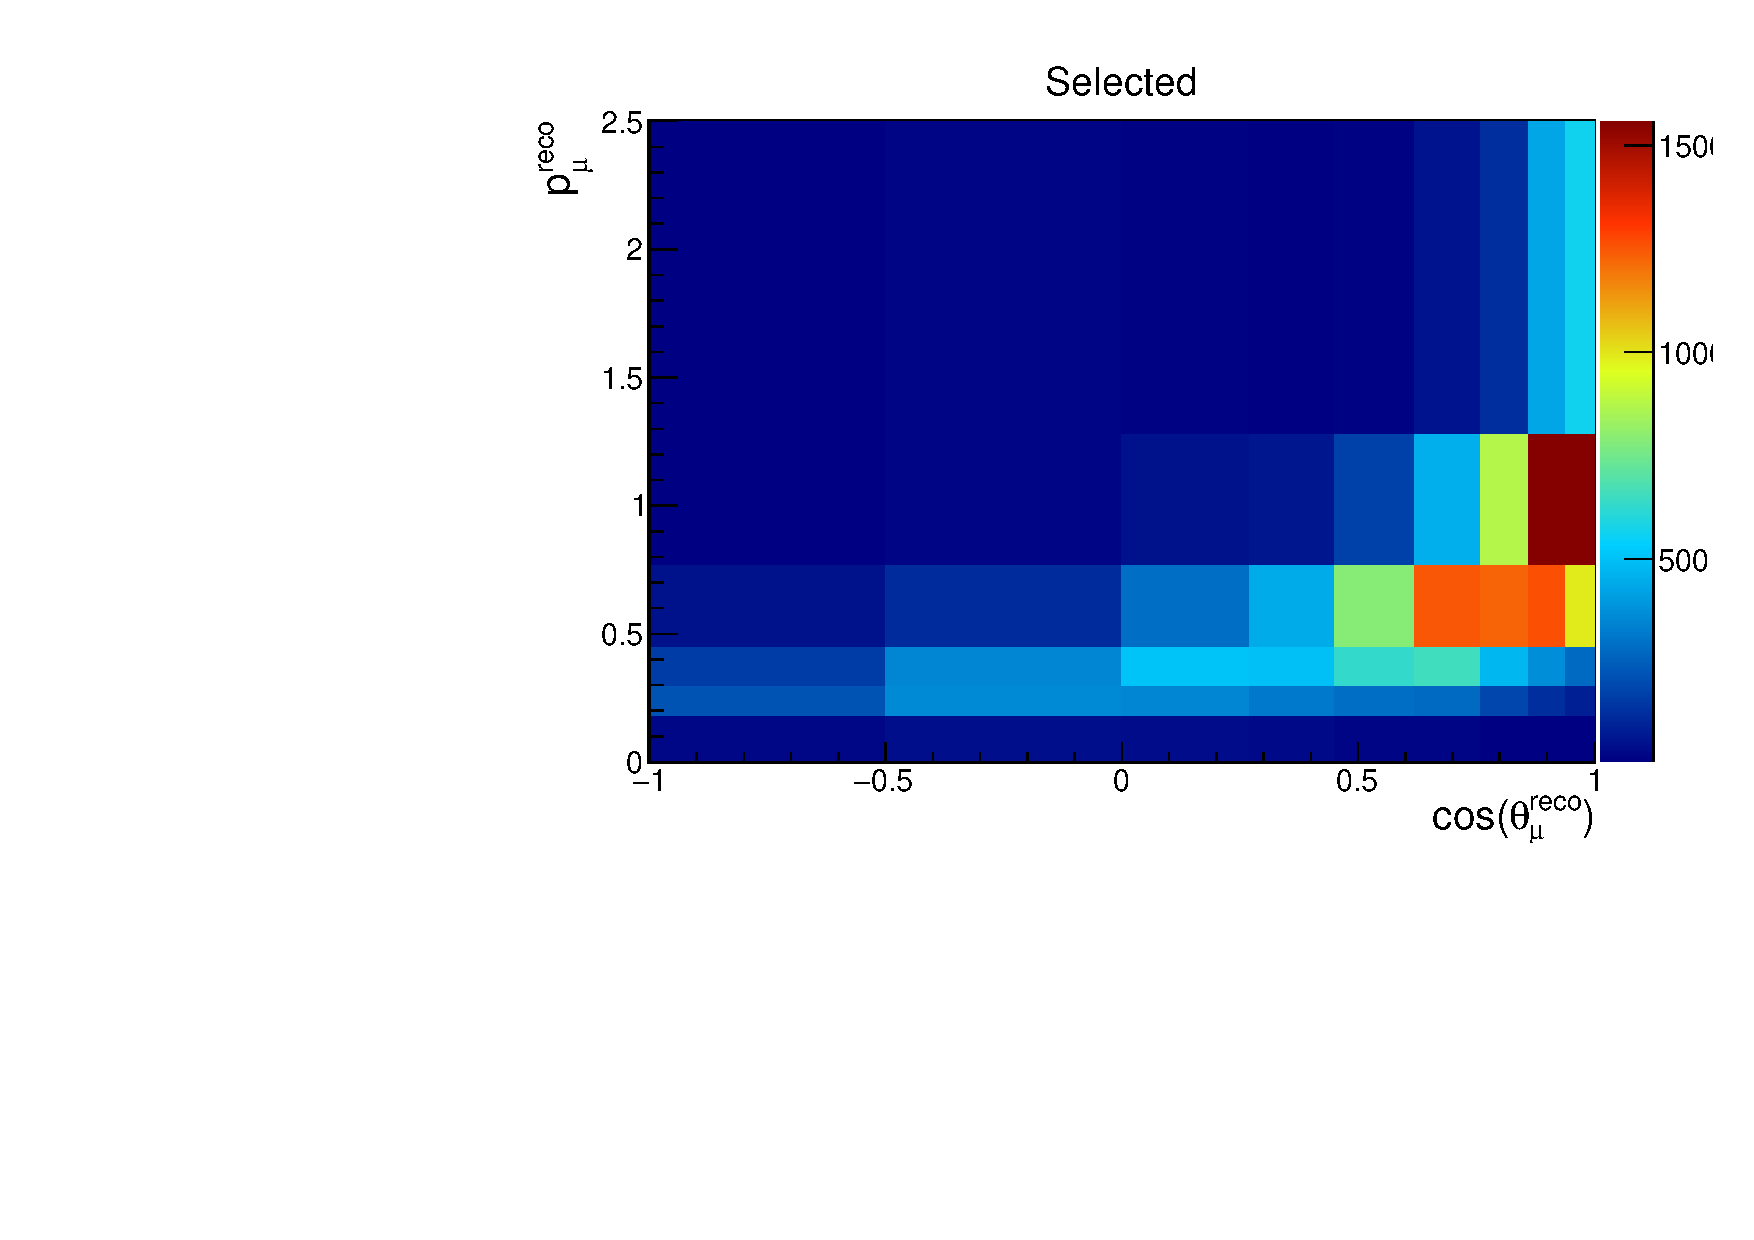
\includegraphics[width=.45\textwidth]{images/XSecPmuCosThetaMu/trkcostheta_trkmumom_selected_smeared}
   \label{fig:trkcostheta_trkmumom_selected_smear}} \quad
\subfloat[][Before smearing.]
   {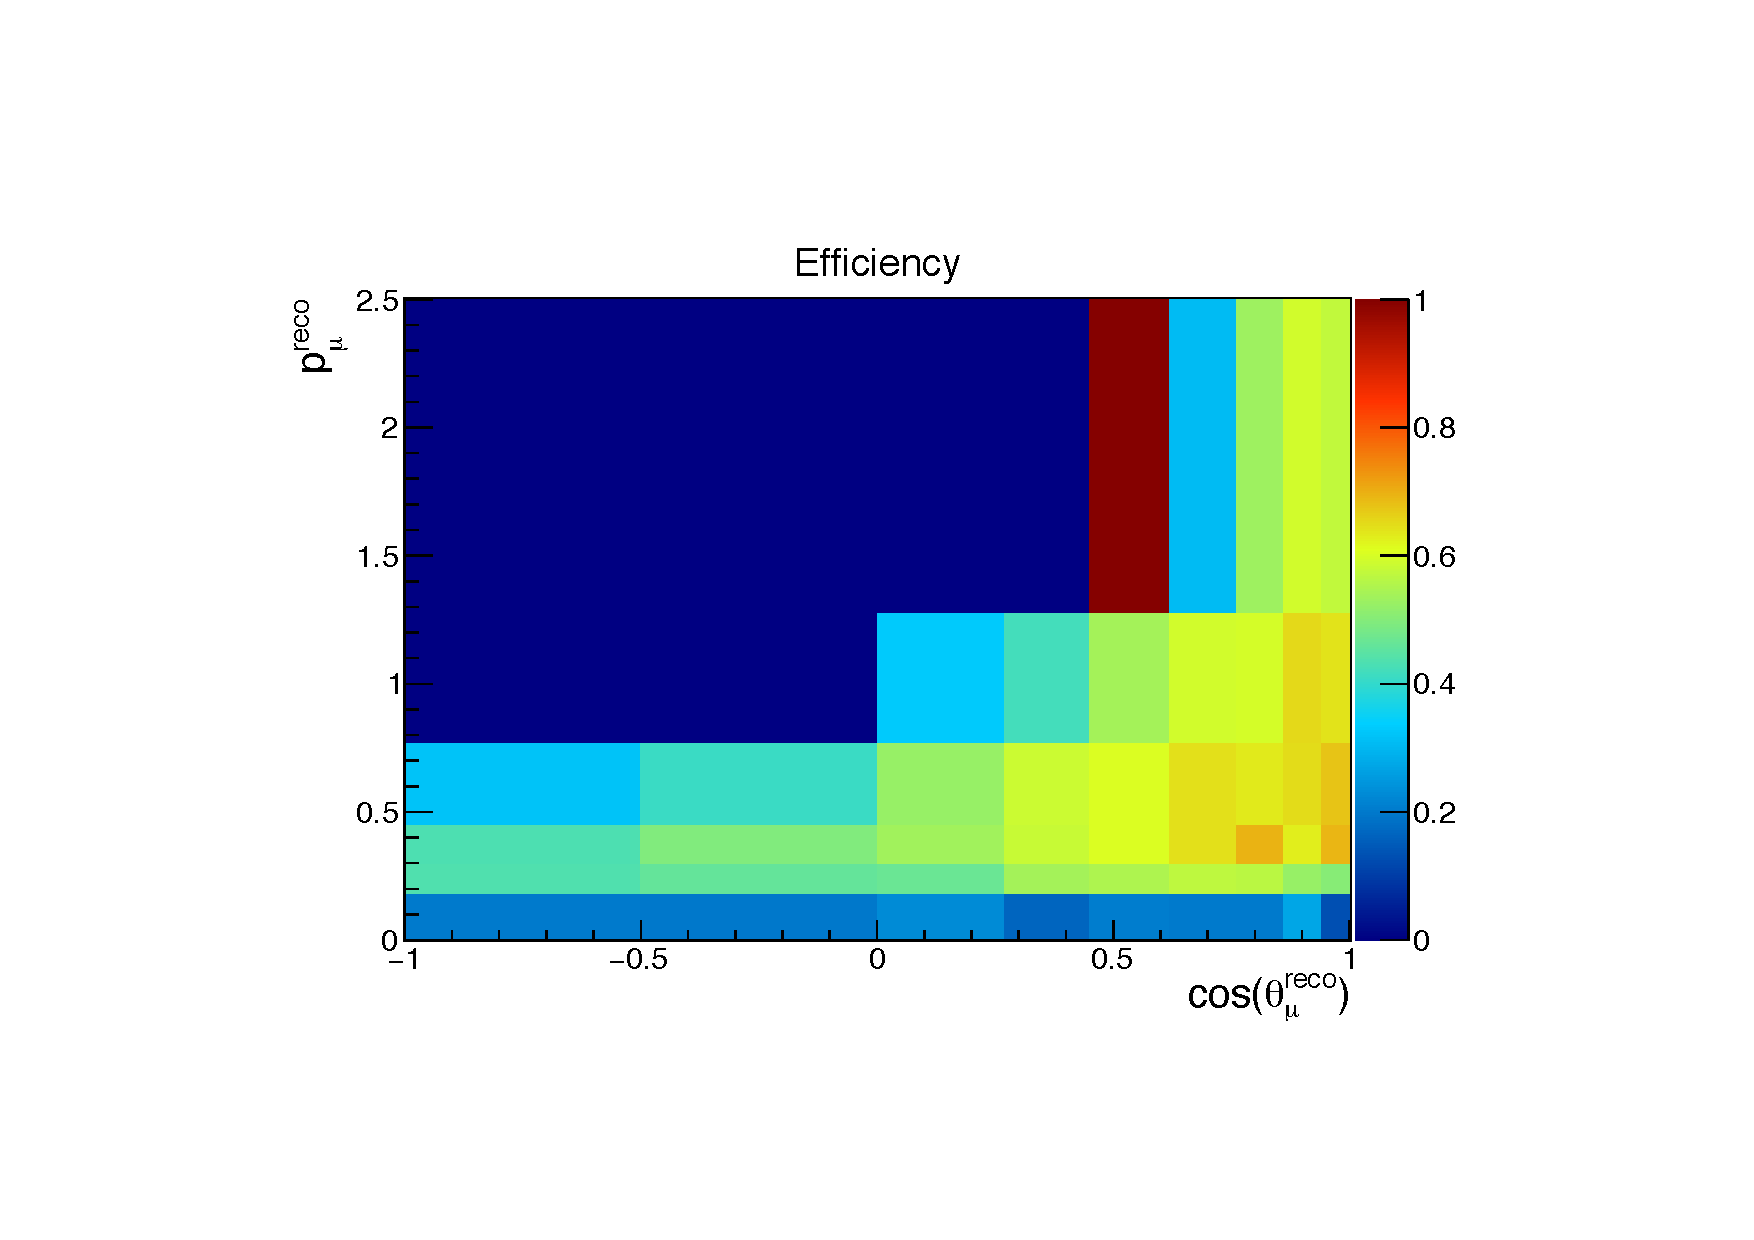
\includegraphics[width=.45\textwidth]{images/XSecPmuCosThetaMu/trkcostheta_trkmumom_efficiency_true_new}
   \label{fig:trkcostheta_trkmumom_efficiecy_true}} \quad
\subfloat[][After smearing.]
   {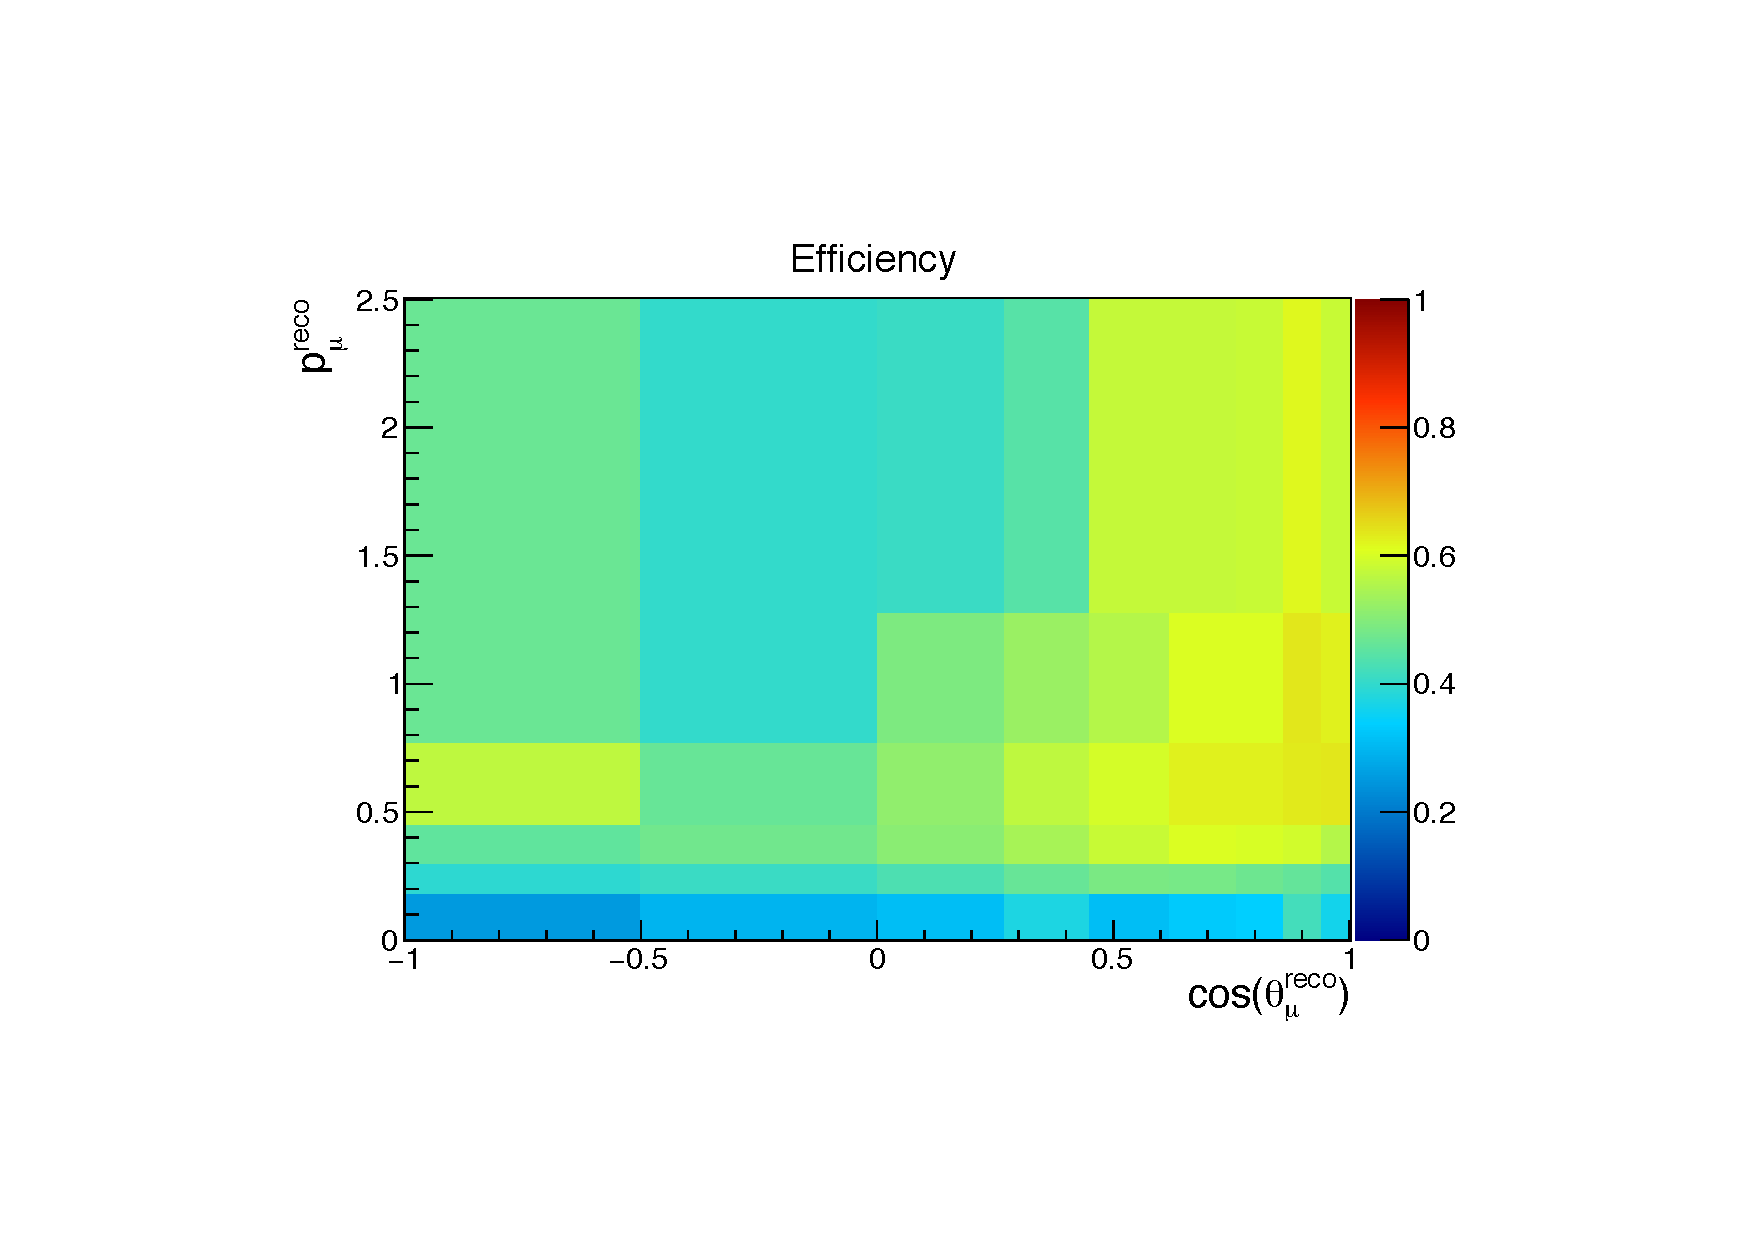
\includegraphics[width=.45\textwidth]{images/XSecPmuCosThetaMu/trkcostheta_trkmumom_efficiency_smear_new}
   \label{fig:trkcostheta_trkmumom__efficiecy_reco}} \\
\caption[Simulated Distributions and Efficiency in $(\cos\theta_\mu, p_\mu)$ Bins]{
Top: distributions of the generated signal events in terms of the simulated variables $(p_\mu^\text{truth}, \cos\theta_\mu^\text{truth})$~\protect\subref{fig:trkcostheta_trkmumom_all} and, after smearing, the reconstructed variables $(p_\mu^\text{reco}, \cos\theta_\mu^\text{reco})$~\protect\subref{fig:trkcostheta_trkmumom_all_smear}. 
Middle: distributions of the selected signal events in terms of the simulated variables $(p_\mu^\text{truth}, \cos\theta_\mu^\text{truth})$~\protect\subref{fig:trkcostheta_trkmumom_selected} and, after smearing, the reconstructed variable $(p_\mu^\text{reco}, \cos\theta_\mu^\text{reco})$~\protect\subref{fig:trkcostheta_trkmumom_selected_smear}.
Bottom: ratio of the distributions above, meaning the efficiency in $(p_\mu^\text{truth}, \cos\theta_\mu^\text{truth})$~\protect\subref{fig:trkcostheta_trkmumom_efficiecy_true} and in $(p_\mu^\text{reco}, \cos\theta_\mu^\text{reco})$~\protect\subref{fig:trkcostheta_trkmumom__efficiecy_reco}.
}
\label{fig:trkcostheta_trkmom_eff_smear}
\end{figure}






%\subsection{Cross Section Central Values}


Putting all the quantities calculated in the previous sections into Equation~\ref{eq:xsec_double_differential}, the $\nu_\mu$ \acrshort{cc} inclusive double-differential cross section on argon is extracted, as shown in Figure~\ref{fig:trkcostheta_trkmumom__xsec_data} for data and in Figure~\ref{fig:trkcostheta_trkmumom__xsec_mc} for simulation. Data and simulation are also compared in Figure~\ref{fig:trkcostheta_trkmumom__xsec_anglesplit_stat}. Here, the data extracted cross section is compared to the default \g simulation as well as an alternative \g configuration, as previously described in Section~\ref{sec:simulation}. A more detailed comparison between these two simulations will be made in Chapter~\ref{ch:cross_section_results}, once systematic uncertainties are incorporated into the analysis.

\begin{figure}[]
\centering
\subfloat[][Data.]
   {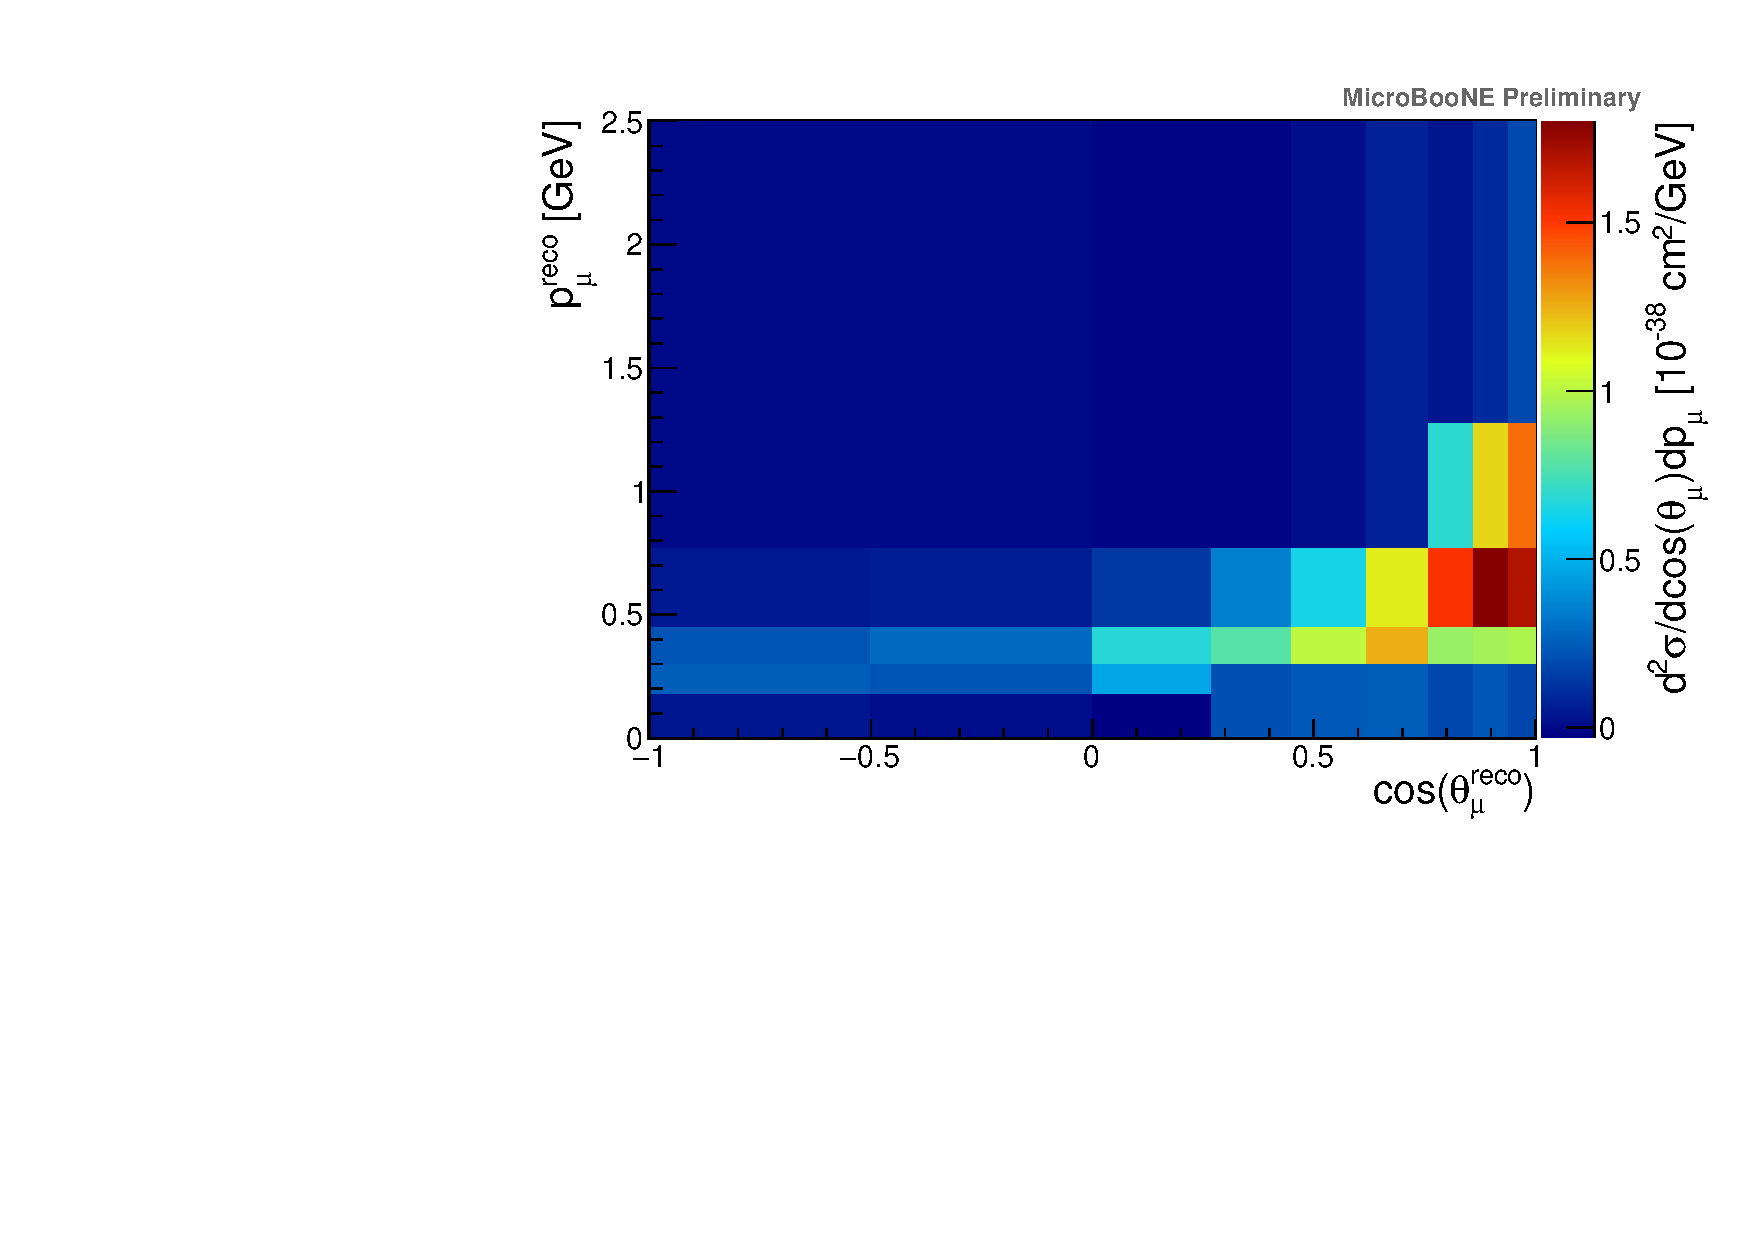
\includegraphics[width=.65\textwidth]{images/XSecPmuCosThetaMu/trkcostheta_trkmumom__xsec_data}
   \label{fig:trkcostheta_trkmumom__xsec_data}} \qquad
\subfloat[][Simulation.]
   {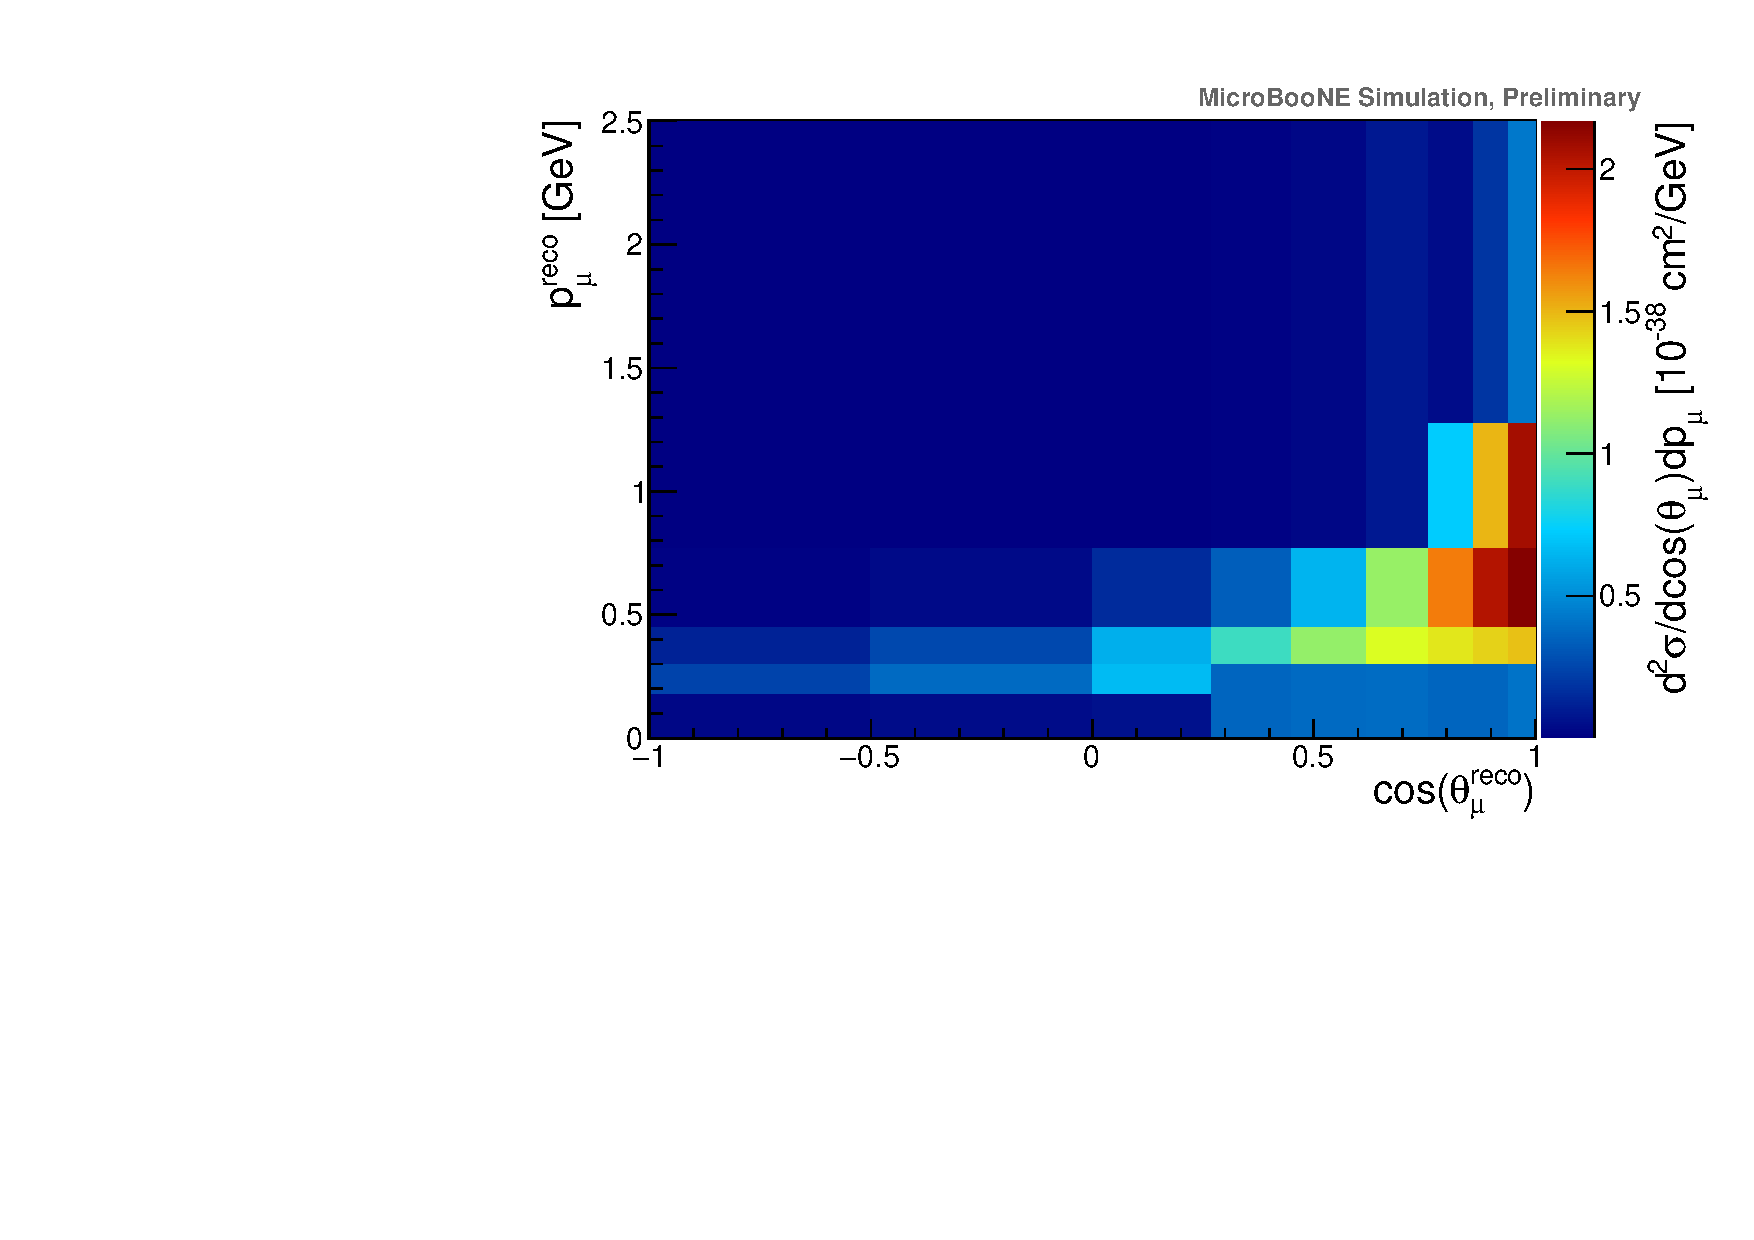
\includegraphics[width=.65\textwidth]{images/XSecPmuCosThetaMu/trkcostheta_trkmumom__xsec_mc}
   \label{fig:trkcostheta_trkmumom__xsec_mc}} \\
\caption[$\nu_\mu$ CC Double-Differential Cross Section (2D View)]{$\nu_\mu$ \acrshort{cc} inclusive double-differential cross section on argon per nucleon as a function of the reconstructed muon momentum and cosine of the reconstructed muon polar angle (angle with respect to the incoming neutrino direction). The data extracted cross section is shown in Figure~\protect\subref{fig:trkcostheta_trkmumom__xsec_data}, while the \acrshort{mc} prediction is shown in Figure~\protect\subref{fig:trkcostheta_trkmumom__xsec_mc}. Only central values are shown in these plots.}
\label{fig:trkcostheta_trkmumom__xsec}
\end{figure}

\begin{figure}[]
\centering
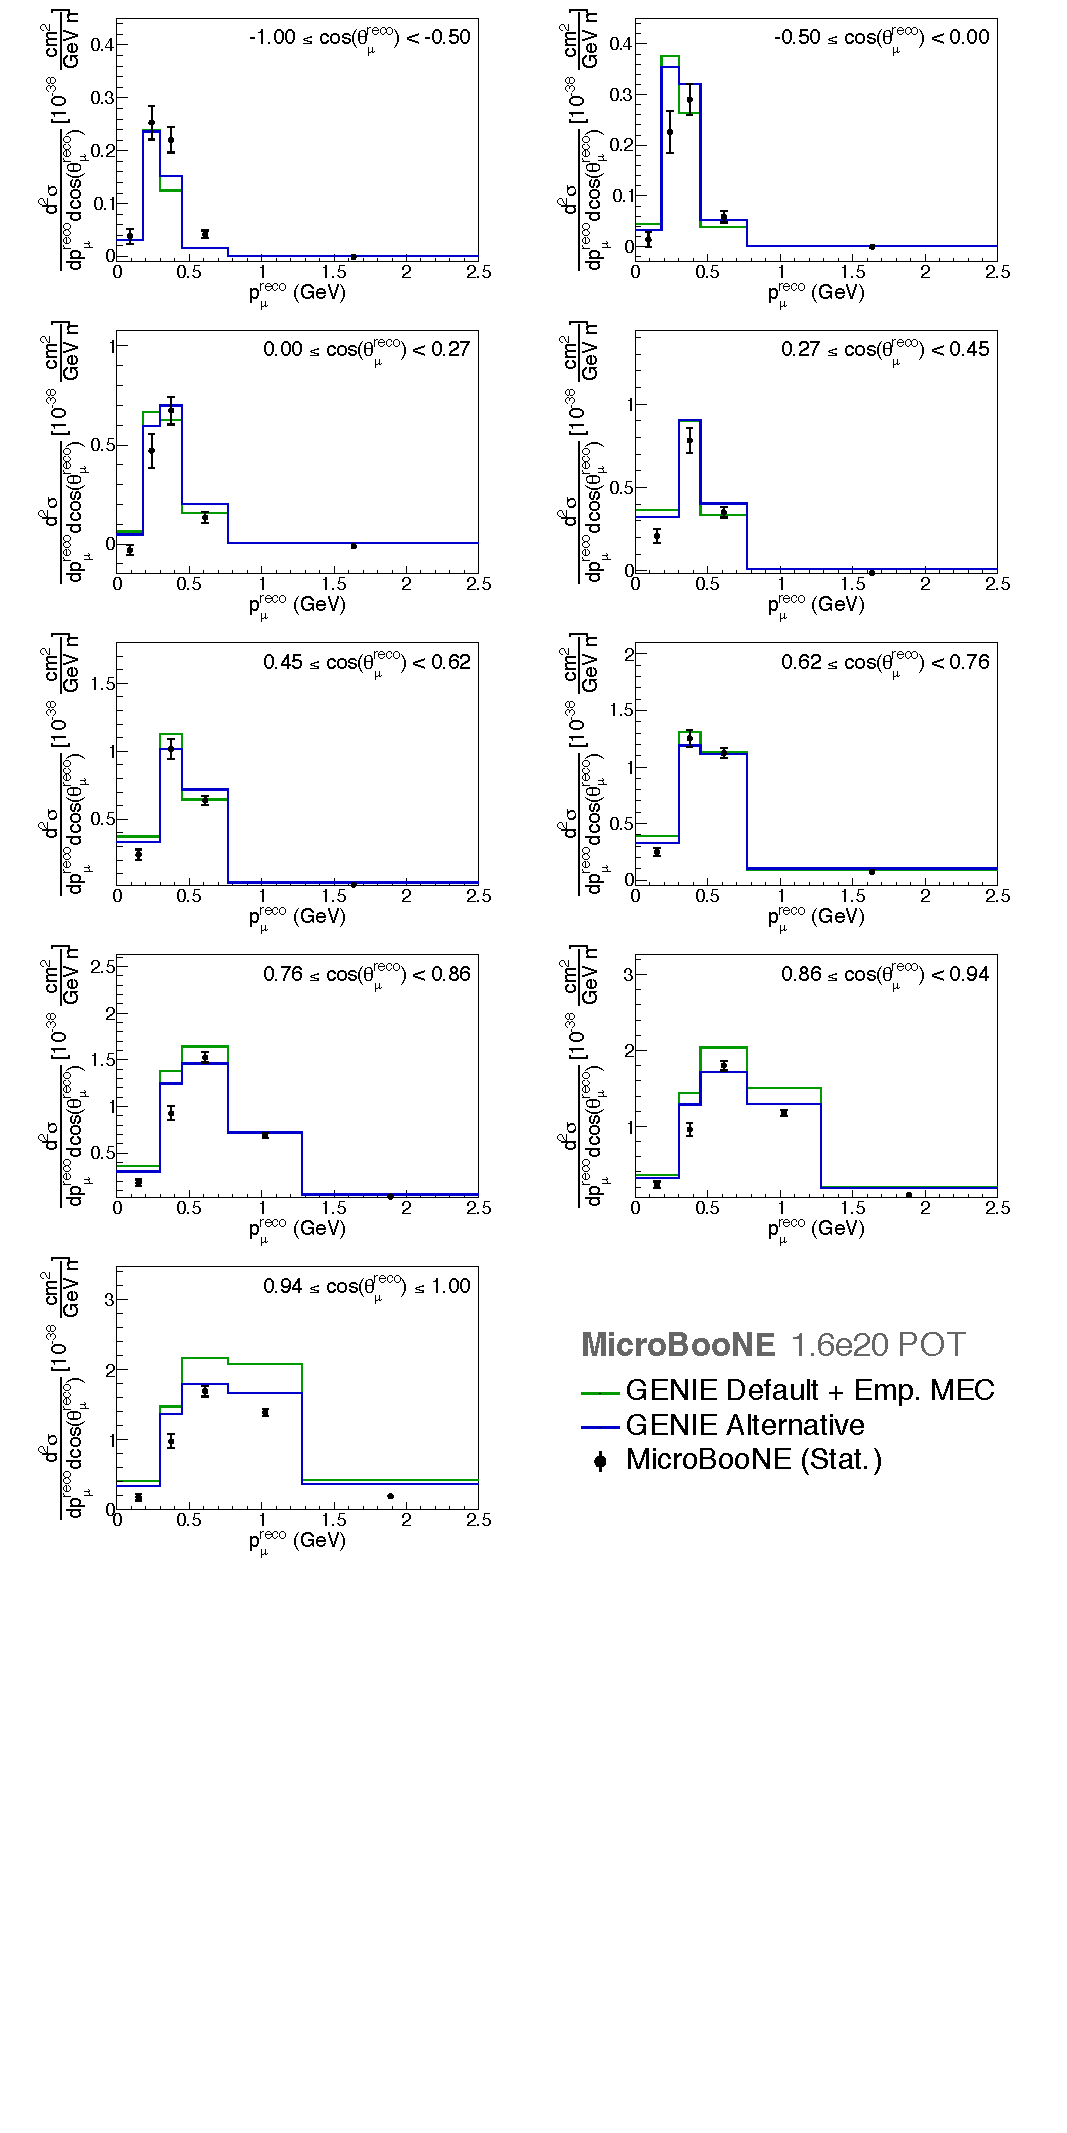
\includegraphics[width=.85\textwidth]{images/XSecPmuCosThetaMu/xsec_bigger_stat}
\caption[$\nu_\mu$ CC Double-Differential Cross Section (Stat. Unc. Only, Split in $\cos\theta_\mu$ Bins)]{$\nu_\mu$ \acrshort{cc} inclusive double-differential cross section on argon per nucleon as a function of the reconstructed muon momentum and cosine of the reconstructed muon polar angle (angle with respect to the incoming neutrino direction). The error bars show statistical uncertainties only. The ``\tuneone'' prediction prediction is shown in green, while the ``\tunethree'' prediction is shown in blue. The error bars show statistical uncertainties only.}
\label{fig:trkcostheta_trkmumom__xsec_anglesplit_stat}
\end{figure}





\section{Cross-Section Extraction Summary}

This chapter presented the procedure used to extract the total, single- and double-differential cross sections.
In order to validate that the analysis framework is functioning correctly and that there are no significant biases in the cross-section results, fake data tests have performed as shown in Appendix~\ref{ch:appendix_validation}.
The next chapter will discuss the systematic uncertainties that affect this measurement, and how they are estimated. The cross section with both statistical and systematic uncertainties will be shown in Chapter~\ref{ch:cross_section_results}.








